\documentclass[12pt,a4paper]{report}
\usepackage[utf8]{inputenc} % Kodierung
\usepackage[ngerman]{babel} % Sprache
\usepackage{graphicx}
\usepackage{float}
\usepackage{fancyhdr}
\usepackage[bottom,hang]{footmisc}
\usepackage{tabularx}

\setlength{\textwidth}{16cm}
%\setlength{\textheight}{25.5cm}
%\setlength{\topmargin}{-2.0cm}
\setlength{\oddsidemargin}{0cm}
\setlength{\evensidemargin}{0cm}


\fancypagestyle{plain}{
\fancyhead{}
\renewcommand{\headrulewidth}{0.0pt}}

\pagestyle{fancy}
\renewcommand{\chaptermark}[1]{\markboth{#1}{}}
\fancyhf{}
\fancyhead[R]{}
\fancyhead[L]{\textbf{\nouppercase\leftmark}}
\fancyfoot[R]{\thepage}
\fancyfoot[L]{}
\renewcommand{\headrulewidth}{0.5pt}
%\renewcommand{\footrulewidth}{0.5pt}

%\date{\today}
%\author{Jens Noack}
%\title{Bericht zum Praxisprojekt 2\\Anbindung von ADTF}

\begin{document}
\begin{titlepage}
\centering
\vfill
{\bfseries\Huge Bachelorarbeit}\\[2cm]
{\bfseries\Large Entwurf und Implementierung eines}\\[0.2cm]
{\bfseries\Large Messsoftware-Adapters für ein}\\[0.2cm]
{\bfseries\Large Fahrerassistenz-Testsystem}\\
\vfill
vorgelegt von
\vfill
{\large Jens Noack}\\
\vfill
in Kooperation mit der\\[0.3cm]
{\large Berner \& Mattner Systemtechnik GmbH}\\
\begin{center}

\includegraphics[scale  = 1]{Darstellungen/B_M_Logo2}
\end{center}
\vfill
\begin{center}\parbox{0cm}{\begin{tabbing}
xxxxxxxxxx \= xxxxxxxx \kill
Hochschule:\quad\quad\quad\quad\quad\quad\quad\quad\quad \= Hochschule Ulm \\
Fakultät: \> Elektrotechnik und Informationstechnik \\
Studiengang: \> Industrieelektronik \\
\> Schwerpunkt Fahrzeugelektronik \\
Semester : \> Wintersemester 2012/2013 \\
Matrikelnummer: \> 31\,000\,97 \\
Erstgutachter: \> Prof. Dr. Norbert Normann \\
Betreuer Firma: \> Dr. Stefan Wappler
\end{tabbing}}
\end{center}

%\begin{tabbing}
%Matrikelnummer:\quad\quad\quad\quad\quad\quad \= 31\,000\,97 \\
%Betreuer Hochschule: \> Prof. Dr. Norbert Normann \\
%Betreuer Firma: \> Dr. Stefan Wappler
%\end{tabbing}

\end{titlepage}
\addcontentsline{toc}{chapter}{Kurzfassung} %sorgt für eintrag ins inhaltsverzeichnis
\chapter*{Kurzfassung} %  *-> erstellt unnummeriertes chapter

%\section*{Kurzfassung}
%\markboth{Kurzfassung}{Kurzfassung} 

Der reale Test von Fahrerassistenzsystemen ist sehr kompliziert und aufwendig, da er kaum durch entsprechende Tools unterstützt wird. Mit dem ATS wurde im Vorfeld ein Konzept für ein Testsystem entwickelt, was diese Tests deutlich erleichtern soll. Der Hauptvorteil liegt darin, dass konsistente Daten aufgezeichnet werden und der Testfahrer während der Fahrt durch ein Tablet unterstützt wird. Mit Hilfe der Online-Auswertung wird der Fahrer durch den Testfall geführt und bekommt Rückmeldungen über die Korrektheit der ausgeführten Manöver. Diese Arbeit beschäftigt sich mit der Konzeptionierung des Systems zur Messdatenerfassung und -auswertung. Dazu wurde ein Software-Modul entworfen und umgesetzt, das die automatisierte Messdatenaufzeichnung unterstützt und die Online-Auswertung bereitstellt.

Zur Erfüllung dieser Funktionen wird ein Laptop genutzt, auf dem die Software ADTF verwendet wird. Mit ADTF werden die Messdaten (CAN-Daten) aufgenommen und ausgewertet. Über die Scrip\-ting\--Schnitt\-stelle (Python-Skripte) von ADTF wird ein Software-Adapter eingebunden, über den ADTF drahtlos durch ein Tablet gesteuert werden kann. Sowohl Laptop als auch Tablet sind per WLAN, das durch einen WLAN-Router zur Verfügung gestellt wird, verbunden. Durch das Python-Skript wird ein TCP-Server generiert, über den der Adapter angesprochen werden kann. Werden entsprechende Nachrichten an diesen Server gesendet, steuert der Adapter ADTF. Die Steuerung umfasst Befehle, um die Messung zu verwalten (z.B. starten und stoppen) und Online-Auswertungen anzufordern. Zur Durchführung der Online-Auswertung wird ein Filter in der ADTF Konfiguration verwendet, dessen Implementierung allerdings nicht zum Arbeitsumfang dieser Arbeit gehört. Die gesendeten Antworten des Adapters ermöglichen dem Tablet, den Testfahrer durch den Testfall zu führen.
%\begin{abstract}
%Zusammenfassung der Arbeiten ....
%\end{abstract}
\tableofcontents
\newpage
\chapter{Einleitung}\label{chap:Einleitung}
Einer der am stärksten wachsenden Wirtschafts- und Industriezweige der letzten Jahrzehnte war die Elektrotechnik. Speziell auf dem Gebiet der Mikroelektronik hat sich in dieser Zeit, vor allem in Bezug auf Integration und Performance, sehr viel verändert. Die Mikro-Chips sind somit nicht nur immer leistungsfähiger, sondern auch immer kleiner geworden. Dieser Trend ermöglicht auch in anderen Bereichen weitreichende Veränderungen und stellt den Grundstein für neue Innovationen dar. 

Auch vor der Automobilindustrie hat diese Entwicklung nicht halt gemacht und so hat vor allem die Entwicklung von Fahrerassistenzsystemen (FAS) davon profitieren können. Die Verarbeitung von Video- und Bilddaten, der komplizierte Rechenalgorithmen zugrunde liegen, kann heutzutage durch neue leistungsfähige Mikroprozessoren während der Fahrt in Echtzeit durchgeführt werden. Mit Hilfe von neuen FAS kann das Fahrzeug seine Umgebung "`wahrnehmen"' und bei Bedarf darauf reagieren. Diese neuen FAS können somit sicherheitsrelevante Aufgaben übernehmen und z.B. bei Bedarf in die Lenkung eingreifen oder eine Notbremsung einleiten. Übergibt man elektronischen Systemen jedoch so viel Kontrolle über das Fahrzeug, muss die korrekte Funktionsfähigkeit des Systems sichergestellt werden. Deswegen durchlaufen FAS während ihrer Entwicklung unzählige Tests, um sie in allen nur erdenklichen Situationen zu erproben. Viele dieser Tests können dabei automatisiert durchgeführt werden. Die reale Testfahrt auf "`offener Stra\ss e"' ist durch diese Testverfahren jedoch nicht komplett zu ersetzen, und nimmt immer noch einen hohen Anteil bei der Erprobung ein. 

Problematisch ist dabei jedoch, dass besonders diese realen Testfahrten kaum durch geeignete Tools unterstützt werden, was sich äu\ss erst negativ auf den Zeit- und Personalaufwand auswirkt. Meist werden einfachste Mittel verwendet, um eine Testfahrt durchzuführen. So liegt die Testspezifikation, welche die auszuführenden Fahrmanöver auflistet, meist in Form einer Excel-Tabelle vor. Diese Tabelle wird vom Beifahrer verwaltet, der dem Testfahrer die Manöver benennt. Dabei gibt es nicht selten Interpretationsspielräume, die falsch ausgeführte Testfahrten und damit unbrauchbare Messdaten zur Folge haben. Um die Testfahrten später den Testfällen zuordnen zu können, wird während der Testfahrt ein Testprotokoll erstellt, welches meist papierbasiert ist. In diesem Testprotokoll wird unter anderem festgehalten, wann ein neuer Testfall beginnt und welche speziellen Bedingungen bei der Testfahrt vorliegen. Die spätere Zusammenführung der Daten ist sehr schwierig und hängt stark von der korrekten Arbeitsweise des Beifahrers ab, der die Dokumentation erstellt hat. Die Zuordnung der Messdaten zu den einzelnen Testfällen erfolgt meist händisch durch die Analyse des Testprotokolls.

Dieses Vorgehen hat eine sehr schwierige, fehlerhafte und zeitraubende Handhabung und erfordert zudem eine gute Ausbildung der Testfahrer. Es provoziert Inkonsistenzen der Messdaten und macht die Zuordnung von Testergebnissen zu den Testfällen sehr schwer. Die wesentliche Schwachstelle dieses Vorgehens ist die fehlende Durchgängigkeit und das fehlende einheitliche Gesamtkonzept.

Bei der Firma Berner \& Mattner entwickelt man momentan ein System, welches zur Verbesserung dieser Situation beiträgt. Es wurde bereits ein Konzept erarbeitet, welches auch die Ausgangssituation dieser Arbeit darstellt und zum Anfang der Bearbeitung dieser Arbeit parallel vertieft wird. Dieses Grundkonzept beschreibt ein vierteiliges System, welches die Vorgehensweise bei Testfahrten verbessert. Mit seinen vier Komponenten soll das Tool den Test vereinfachen, indem sowohl die Testfallerstellung, die Testfalldurchführung und die anschließende Auswertung unterstützt werden. Besonders die Durchführung der Testfahrt vereinfacht sich durch das System, da diese dann komplett rechnergestützt durchgeführt wird. Dazu wird ein Tablet verwendet, mit dessen Hilfe der Testfahrer durch die Testfahrt geführt wird. Das Tablet gibt dem Testfahrer Informationen zur Testfahrt und übernimmt gleichzeitig auch die Bedienung der Messtechnik. Zur Veranschaulichung dient die Schemadarstellung in Abbildung \ref{pic:Konzept}.
\begin{figure}
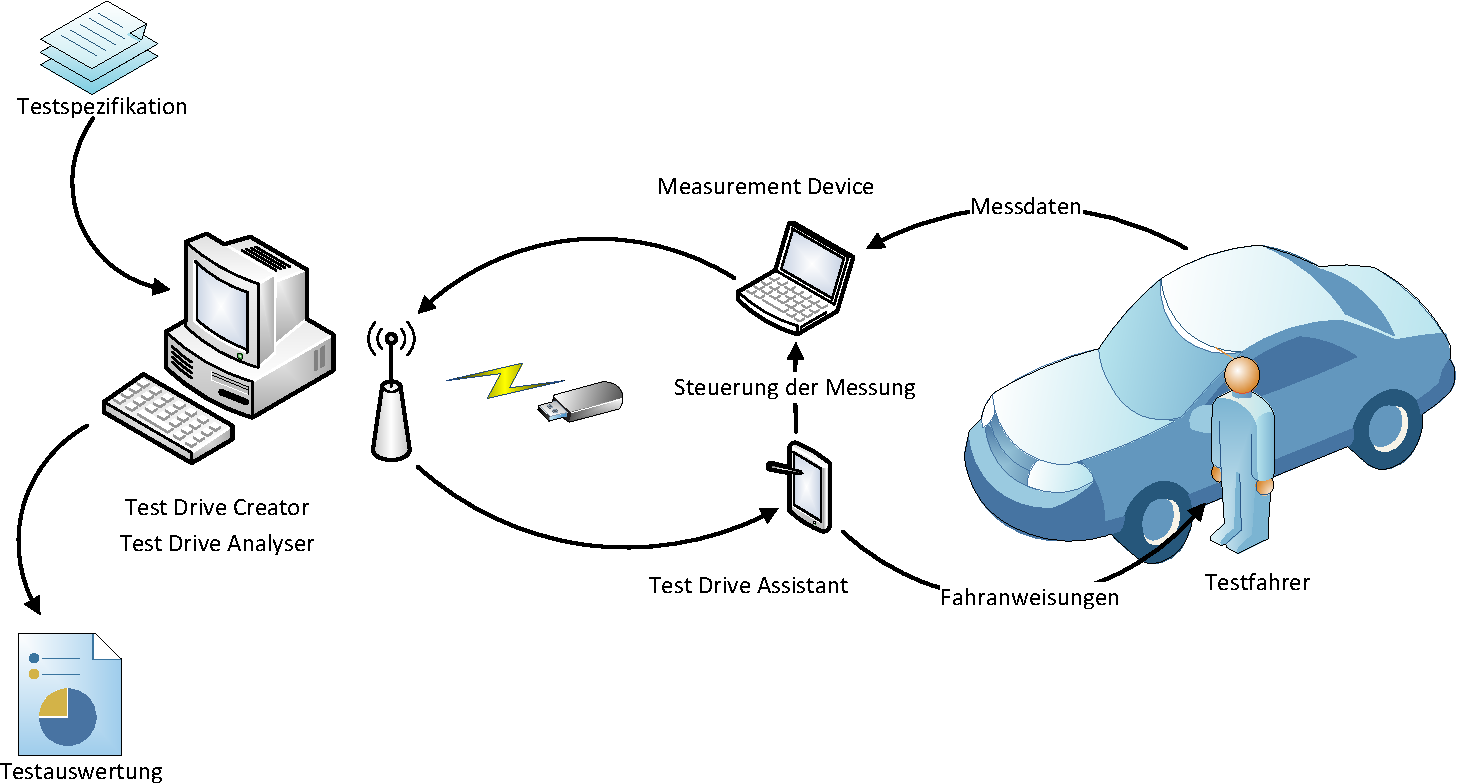
\includegraphics[width=1\linewidth]{Darstellungen/Uebersicht_System}
\caption{Übersicht Grundkonzept (in Anlehnung an Testkonzept Fahrerarbeitsplatz)}\label{pic:Konzept}
\end{figure}
\noindent Wie der Darstellung zu entnehmen ist, besteht das System aus folgenden vier Komponenten:
\begin{itemize}
\item{Test Drive Creator}
\item{Test Drive Analyser}
\item{Test Drive Assistant}
\item{Measurement Device}
\end{itemize}
Im Zuge der Vertiefung des ersten Konzeptes wurden teilweise die Namen der Komponenten abgeändert, um ihre Aufgaben besser abzubilden. Der Test Drive Creator dient im Kern dazu, eine Testfahrt vorzubereiten. Um dies zu gewährleisten, müssen die für den Test Drive Assistant (TDA) notwendigen Daten generiert werden. Grundlage dieser Daten ist die Testspezifikation, bestehend aus Testkampagnen\footnote{eine Zusammenstellungen von mehreren Testfällen}. Mit dem Creator hat man sowohl die Möglichkeit fertige Testspezifikationen, die mit anderer Software erstellt wurden, einzubinden als auch eigene Spezifikationen zu erstellen. Zum Erstellen der Testspezifikation wird dabei die Software CTE\footnote{der Classification Tree Editor von der Fa. Berner \& Mattner dient zur Erstellung von Testspezifikationen nach der Klassifikationsbaum-Methode} verwendet.

Mit dem Test Drive Analyser soll nach abgeschlossener Testfahrt die Möglichkeit bestehen, die Messdaten zu verarbeiten und auszuwerten. Im ersten Prototyp wird diese Funktion allerdings noch nicht umgesetzt. Die beiden beschriebenen Komponenten werden auf einem herkömmlichen Desktop PC ausgeführt.

Das Herzstück des Testsystems bilden jedoch der Test Drive Assistant (TDA) und das Measurement Device. Diese beiden Komponenten ermöglichen einen komfortablen Testdurchlauf und generieren die Messdaten. Dazu leitet der TDA den Testfahrer durch Hinweise auf dem Bildschirm durch die Testfahrt und steuert währenddessen die Messung durch das Measurement Device. Der Testfahrer muss sich während der Fahrt somit nicht um die Messtechnik oder die korrekte Dokumentation der Messdaten kümmern. Er muss lediglich den Anweisungen auf dem Tablet folgen und kann Kommentare und Anmerkungen zu den Messungen einfügen. Um den Fahrer möglichst gut zu unterstützen, sollen einzelne Testfälle in mehrere messbare Bedingungen unterteilt werden, dessen Erreichen das Weiterschalten der Testfahrt herbeiführen. Der Testfahrer hat dadurch schon während der Testfahrt eine direkte Kontrolle darüber, ob die Testfahrt korrekt durchgeführt wird. Um diese Funktionalität zu bieten, ist eine Art Online-Auswertung der Fahrzeugdaten notwendig.
\section{Ziele dieser Arbeit}
Ziele dieser Arbeit sind der Entwurf, die prototypische Implementierung und der Test des Measurement Devices, des bereits beschriebenen Gesamtkonzeptes. Ausgeschlossen hiervon ist die Umsetzung der Online-Analyse. Abbildung \ref{pic:Grobdarstellung Systemkonzept} zeigt eine Grobdarstellung des Konzeptes auf Systemebene, in der die umzusetzende Komponente markiert ist.
\begin{figure}[H]
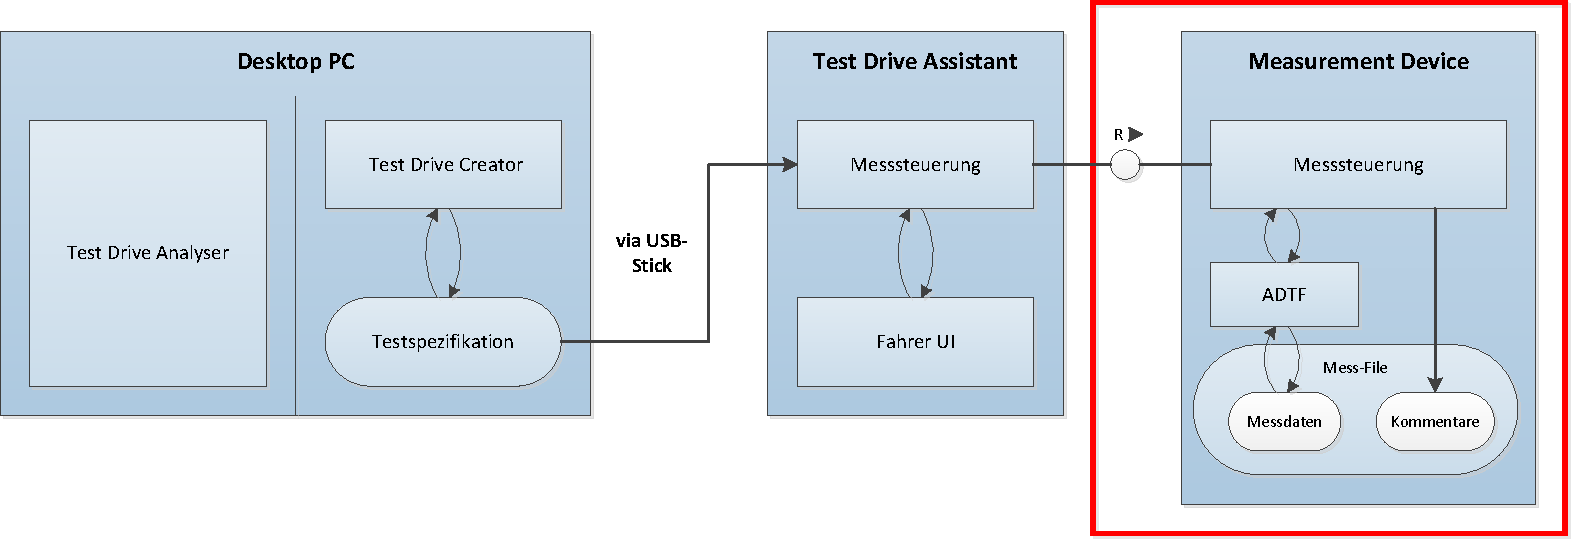
\includegraphics[width=1\linewidth]{Darstellungen/Systemuebersicht-Einleitung}
\caption{Grobdarstellung Systemkonzept}\label{pic:Grobdarstellung Systemkonzept}
\end{figure}
\noindent Dies beinhaltet den Konfigurationsentwurf der Messtechnik und deren Anbindung an den TDA. Zur Aufnahme der Fahrzeugdaten soll die Software ADTF, von der Firma Elektrobit, verwendet werden. ADTF soll durch den TDA steuerbar sein. Dazu soll ein geeignetes Konzept für die Kommunikation entwickelt und umgesetzt werden. Durch die Kommunikation soll es möglich sein, allgemeine Steuerbefehle zu senden, wodurch beispielsweise Konfigurationen geladen und gestoppt oder Messungen gestartet und angehalten werden können. Dabei soll auch die Unterstützung der Online-Auswertung besondere Berücksichtigung finden und in Protokollen eingeplant werden. Um eventuelle Fehler des Systems im späteren Einsatz besser identifizieren zu können, soll ein durchgängiges Fehlermanagement umgesetzt werden.

Als Grundlage dient ein bereits bestehendes Projekt, bei dem ein Adapter für ADTF entwickelt wurde. Dieser Adapter hat die Funktion, ADTF für die Testautomatisierung einzusetzen. Dieses Projekt soll analysiert werden, um Parallelitäten herauszufinden und dadurch gegebenenfalls Arbeitsaufwand einzusparen.
\section{Gliederung der Arbeit}
Diese Arbeit ist unterteilt in fünf Abschnitte. Im ersten Abschnitt wird auf die Grundlagen eingegangen, welche das für diese Arbeit benötigte Wissen kurz zusammenfassen. Das zweite Kapitel beschäftigt sich mit der Anforderungsanalyse der zu entwerfenden Komponente und bildet die Grundlage für den Konzeptentwurf. In den darauf folgenden Abschnitten drei und vier wird der Konzeptentwurf, gefolgt von dessen Umsetzung und dem Test der Funktionen, dargestellt. Das letzte Kapitel fasst die Arbeiten zusammen, gibt eine Bewertung und zeigt Potentiale für anschließende Arbeiten auf. Im Anhang befindet sich eine Bedienungsanleitung für das entworfene System.
\chapter{Grundlagen}\label{chap:Grundlagen}
Um das Verständnis der beschriebenen Probleme sicherzustellen, werden in diesem Kapitel einige technische Grundlagen und projektbezogenes Vorwissen vermittelt.
\section{Systemkonzept ADAS Test System}\label{sec:Systemkonzept ADAS Test System}
Das ADAS\footnote{ADAS - \textbf{A}dvanced \textbf{D}river \textbf{A}ssistance \textbf{S}ystems ist die englische Entsprechung für Fahrerassistenzsysteme (FAS)} Test System (ATS) soll den Test von Fahrerassistenzsystemen wesentlich erleichtern. Das allgemeine Konzept wurde im Vorfeld dieser Arbeit von David Klowersa erstellt und bildet die Grundlage für die weitere Vertiefung. Der frühere Arbeitstitel dieses Projektes war Fahrerarbeitsplatz. Die Unterlagen zum Grundkonzept sind auf der beiliegenden Disc enthalten. In der Einleitung dieser Arbeit wurden bereits die Bedeutung und die Motivation zur Entwicklung dieses Systems dargestellt. An dieser Stelle sollen die Funktionen der einzelnen Komponenten zusammengefasst werden.

Das System ist grundsätzlich auf drei Geräten verteilt. Bei den drei Geräten handelt es sich um einen Desktop PC, ein Android-Tablet und einen Laptop (s. Abb. \ref{pic:Komponentenuebersicht}). Der Desktop PC dient der Erstellung von Testkampagnen sowie der Auswertung der Messdaten. Die Grundlage für eine Testfahrt ist die Testspezifikation. Diese wird mit Hilfe des Test Drive Creators erstellt. Dabei liegt besonderes Augenmerk darauf, dass der Import von bereits bestehenden Testspezifikationen unterstützt wird. Mit bewährten Mitteln, wie dem CTE, kann eine Spezifikation erstellt und importiert werden. Für die Verwendung der Online-Auswertung während der Testfahrt, sollte die Verwendung von CTE zur Erstellung der Spezifikation bevorzugt werden. Bei der Erstellung der Klassifikationsbäume müssen Konventionen eingehalten werden, da durch definierte Konstrukte die Bedingungen für die Online-Auswertung festgelegt werden. Durch eine spezielle Struktur können die Weiterschaltbedingungen formuliert werden. Allerdings gibt es für die Erstellung der Spezifikation noch kein festgelegtes Konzept. Auch für die Datenauswertung gibt es aktuell nur sehr oberflächliche Überlegungen, aber noch kein konkretes Konzept.
\begin{figure}
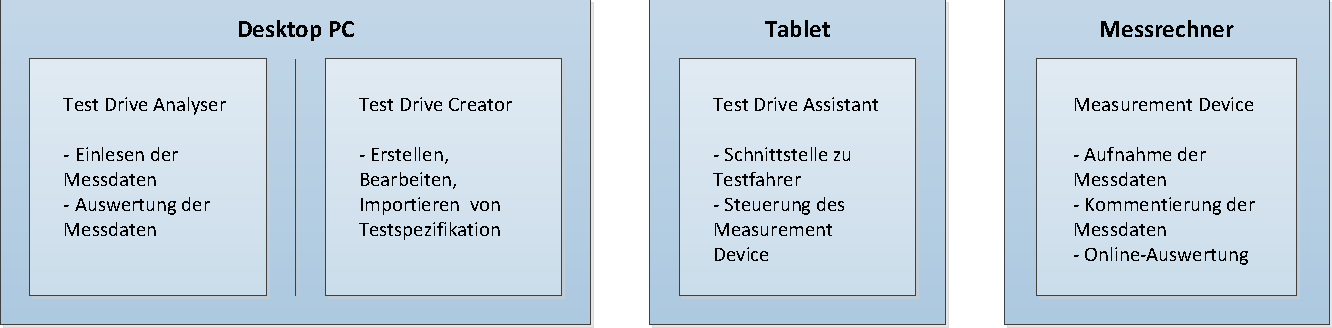
\includegraphics[width=1\linewidth]{Darstellungen/Systemuebersicht-Grundlagen}
\caption{Komponentenübersicht ATS}\label{pic:Komponentenuebersicht}
\end{figure}
Auf dem Android-Tablet ist ein Programm (App) installiert, was die Durchführung der Testfahrt unterstützt. Die mit dem Test Drive Creator erstellte Testkampagne wird auf das Tablet übertragen (beispielsweise per USB Stick) und dort geladen. Die App dient als Schnittstelle zum Testfahrer und besitzt als solche eine grafische Benutzerschnittstelle (GUI\footnote{GUI - \textbf{G}raphical \textbf{U}ser \textbf{I}nterface}). Über diese Schnittstelle leitet der Test Drive Assistant (TDA) den Testfahrer durch die Testfahrt, indem er ihm mitteilt, welches Manöver als nächstes durchgeführt werden soll. Dazu signalisieren geeignete Ausgaben auf dem Bildschirm, was zu tun ist. 

Mit dem Messrechner werden die Messwerte (Fahrzeugdaten) aufgezeichnet. Dazu wird die Software ADTF verwendet, die folgend auch als Measurement Tool bezeichnet wird. Das Measurement Tool ist über den Measurement Adapter an den TDA angebunden. Der Measurement Adapter regelt die Kommunikation und steuert die Aufnahme sowie die Online-Auswertung der Messdaten.

Während der Testfahrer den Anweisungen auf dem Bildschirm folgt, wird die Messdatenaufzeichnung durch den TDA gesteuert. Die Datenaufzeichnung wird von einem Laptop durchgeführt, der sich beispielsweise im Kofferraum des Testfahrzeuges befindet und an den CAN-Bus angeschlossen ist. Die Kommunikation zwischen beiden Komponenten erfolgt dabei über ein Funknetz. Durch die Kommunikation zwischen TDA und Measurement Device wird die komplette Messdatenaufzeichnung gesteuert und damit die Bedienung der Software auf dem Messrechner durchgeführt. Während der Testfahrt hat der Fahrer die Möglichkeit, den Messungen Kommentare hinzuzufügen. Diese Kommentare werden über das Tablet eingegeben und zusammen mit dem Mess-File gespeichert. 

Durch die Online-Auswertung kann sichergestellt werden, dass der Testfahrer die Fahrmanöver richtig durchführt. Eine Testfahrt kann sich dabei aus mehreren Bedingungen zusammensetzen, die für das Fortführen der Testfahrt erfüllt werden müssen. Erst nachdem der Testfahrer einen bestimmten Zustand des Fahrzeuges herbeigeführt hat, kann die Testfahrt durchlaufen und später abgeschlossen werden. Im Folgenden werden diese Bedingungen auch als Weiterschaltbedingungen bezeichnet. Für die Überprüfung dieser Bedingungen können die aktuellen Messdaten durch das Measurement Device ausgewertet werden. Dazu sendet der TDA an das Measurement Device die Aufforderung für die entsprechende Auswertung, und erhält darauf die entsprechenden Antworten. Erst nachdem eine Überprüfung erfolgreich abgeschlossen wurde, kann die Testfahrt fortgeführt werden.
\section{ADTF}\label{sec:ADTF}
Fahrerassistenzsysteme bestehen in der Regel nicht nur aus einem einzigen Modul, sondern aus dem komplizierten Zusammenspiel von Hardware und Software. Durch immer kompliziertere Funktionen wird auch die Software immer komplexer. Um die Entwicklung zu vereinfachen, wurde die Software ADTF entwickelt. ADTF wird seit 2001 von der Audi Electronics Venture (AEV) GmbH entwickelt und seit 2008 durch die Firma Elektrobit (EB) vertrieben. Im VW-Konzern ist ADTF mittlerweile stark verbreitet und erleichtert die Entwicklung von FAS vom Entwurf des ersten Konzepts bis zur Serienentwicklung \cite{AEV}.

Sämtliche Informationen bezüglich ADTF, die für den Entwurf des Konzeptes und die Implementierung des ADTF Adapters nötig waren, wurden der Dokumentation von ADTF entnommen \cite{ADTFDokuUsers}\cite{ADTFDokuDevelopers}\cite{ADTFDokuSDK}. Für weitere Informationen zu ADTF können die soeben genannten Quellen zurate gezogen werden.
\subsection{Vorstellung der Software}\label{subsec:Vorstellung der Software}
Der wesentliche Vorteil von ADTF in Bezug auf dieses Projekt ist die Datenaufzeichnung. In ADTF ist es besonders komfortabel Messdaten aufzuzeichnen, da mehrere Datenströme zeitsynchron aufgezeichnet werden. Die Datenströme erhalten dabei den gleichen "`Zeitstempel"', wodurch die spätere Analyse der Daten wesentlich einfacher ausfällt. Zudem werden die parallel aufgezeichneten Daten in einer einzigen Datei abgelegt. Diese Messdaten können über Dateieigenschaften des Mess-Files kommentiert werden. Dadurch erhält man für eine Testfahrt eine einzige Datei, in dem alle Kommentare abgespeichert werden können. Werden auch diese vom Benutzer erstellten Kommentare mit einem Zeitstempel versehen, so sind alle Daten konsistent und können sehr komfortabel ausgewertet werden.

In Abbildung \ref{pic:Graphische Benutzeroberflaeche ADTF} ist die Programmoberfläche von ADTF zu erkennen. Mit dem ADTF Control-Panel (1) kann ADTF manuell gesteuert werden. Über die Buttons können Konfigurationen geladen, gestartet oder zum Beispiel angehalten werden. Über den Configuration Editor (2) können Konfigurationen grafisch erstellt werden. Aus dem Component Tree (s. Abb. \ref{pic:Component Tree von ADTF}) können Komponenten per "`Drag \& Drop"' in den Editor gezogen werden. Dort können die einzelnen Komponenten verbunden und bearbeitet werden. Der Component Tree kann über eine Auswahl dort angezeigt werden, wo in der Abbildung der Project Tree (3) dargestellt ist. Der Project Tree veranschaulicht, aus welchen Dateien und Komponenten sich das geladene Projekt zusammensetzt. In der Ausgabekonsole (4) werden Statusmeldungen von ADTF angezeigt.
\begin{figure}
\begin{center}
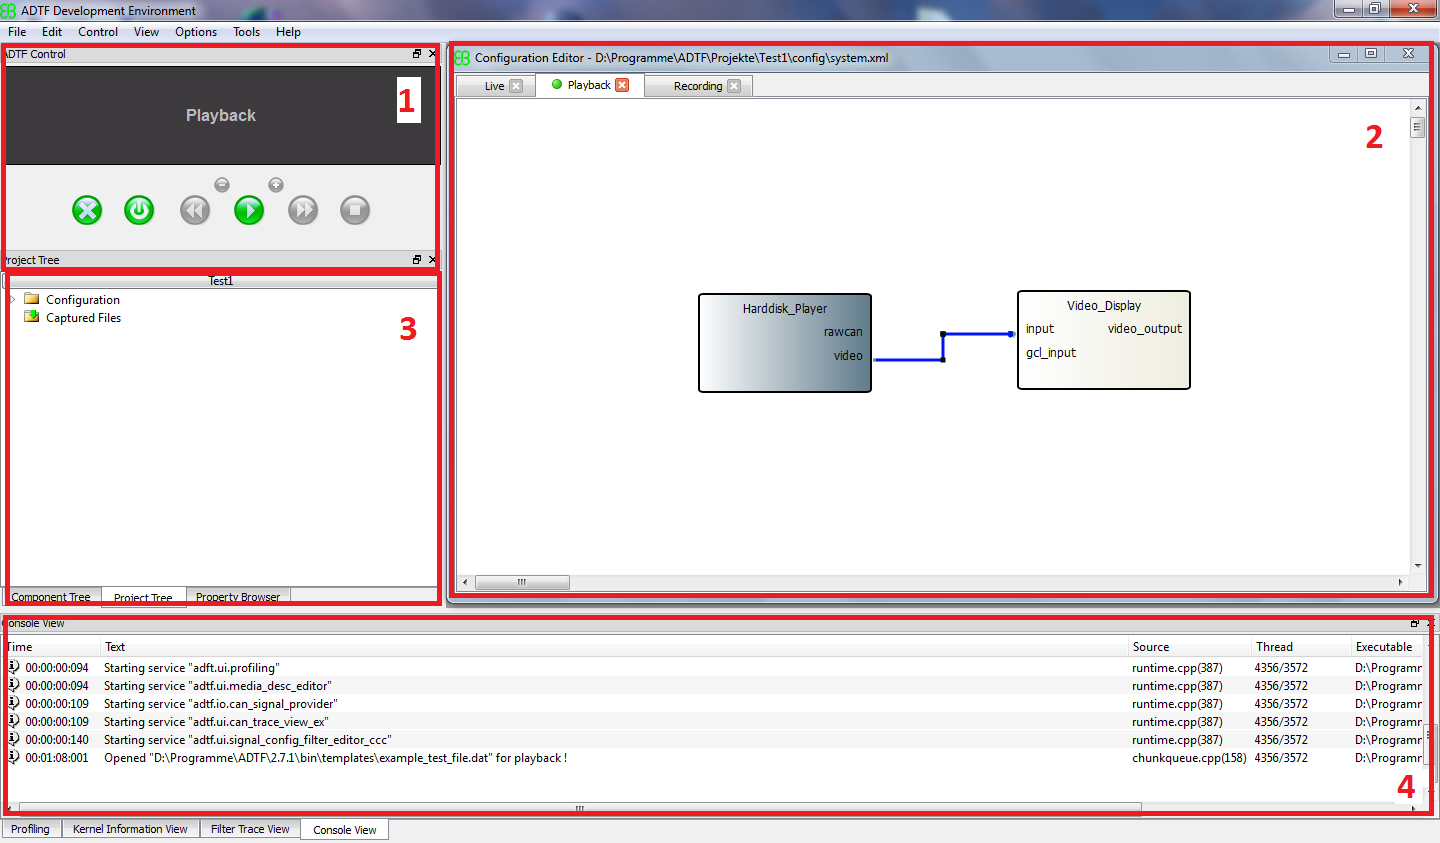
\includegraphics[width=1\linewidth]{Darstellungen/ADTF_uebersicht_markiert}
\caption{Grafische Benutzeroberfläche ADTF}\label{pic:Graphische Benutzeroberflaeche ADTF}
\end{center}
\end{figure}
\begin{figure}
\begin{center}
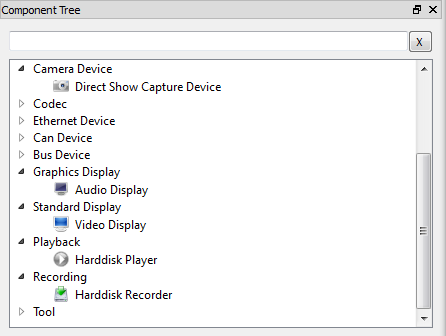
\includegraphics[scale=0.6]{Darstellungen/ADTF_componenttree}
\caption{Component Tree von ADTF}\label{pic:Component Tree von ADTF}
\end{center}
\end{figure}
\subsection{Python-Schnittstelle}\label{subsec:Pythonschnittstelle}
ADTF besitzt eine Scripting-Schnittstelle. Über diese Schnittstelle kann ADTF von einem Skript, das in Python geschrieben wurde, gesteuert werden. Der dazugehörige Service von ADTF trägt den Namen "`Python Support Service"' (PSS). Über die folgende Codezeile kann der Service im Skript importiert werden:
\begin{quote}
\verb|import ADTF|
\end{quote}
Das fertige Skript kann in ADTF importiert und ausgeführt werden. Der PSS besteht aus drei Klassen, welche es ermöglichen auf die grundlegende Steuerung Einfluss zu nehmen. Es können beispielsweise Ausgaben in der Konsole erzeugt oder Konfigurationen geladen und gestartet werden.
\section{Python}\label{sec:Python}
Das Software-Modul, das im Rahmen dieser Abschlussarbeit entsteht, wird in der Programmiersprache Python umgesetzt. Da diese Hochsprache einige Besonderheiten und Eigenheiten gegenüber anderen Hochsprachen besitzt, soll Python an dieser Stelle kurz vorgestellt werden.
\subsection{Vorstellung der Skriptsprache Python}\label{subsec:Vorstellung der Skriptsprache Python}
Python gilt als eine sehr dynamische und flexible Hochsprache. Die Philosophie dieser Hochsprache betont besonders stark die Programmlesbarkeit. Python besitzt eine sehr übersichtliche und einfach zu verstehende Syntax, wodurch die Sprache als einfach zu erlernen gilt. Python ist, wie viele andere Hochsprachen, objektorientiert. Aufgrund seiner hohen Dynamik wird Python oft als Skriptsprache\footnote{Eine Programmiersprache, zur Erstellung von kleinen und überschaubaren Programmen, weswegen auf Sprachelemente verzichtet wird, die erst bei komplexen Programmen eine Rolle spielen. Skripte werden oft direkt interpretiert und nicht erst übersetzt.} verwendet \cite{PythonOrgExecutiveSummary}.
\subsection{Unterschiede zu anderen Hochsprachen}\label{subsec:Unterschiede zu anderen Hochsprachen}
Aus der Zielsetzung, eine besonders hohe Programmlesbarkeit zu erzeugen, ergeben sich einige Unterschiede zu anderen Hochsprachen. Folgend werden einige Besonderheiten, die bei der Implementierung des in dieser Arbeit beschriebenen Moduls verwendet werden, vorgestellt.
\\[0.5cm]
\textbf{Codeeinrückungen}
\\Eines der markantesten Merkmale von Python stellt die Codeeinrückung dar. In Python werden zur Definition von zusammenhängenden Modulen keine Klammern oder Befehle verwendet. Lediglich die Einrückung legt fest, welche aufeinanderfolgenden Codezeilen zu einem Segment (beispielsweise einer Schleife) gehören.
\\[0.5cm]
\textbf{Variablen}
\\Variablen besitzen in Python keinen festen Datentyp, weswegen auch Typdeklarationen überflüssig sind \cite{GalileoPython}. In Python können Variablen wesentlich dynamischer deklariert werden. Variablen können an jeder Stelle des Programms, durch eine einfache Zuweisung eines bestimmten Wertes zu einem bestimmten Variablennamen, erstellt werden.

Python besitzt neben den elementaren Datentypen, die in anderen Hochsprachen ebenfalls vorhanden sind, auch besondere sequenzielle Datentypen. Ein sequenzieller Datentyp beinhaltet Folgen von gleichartigen oder verschiedenen Elementen. Ein bekanntes Beispiel dafür wäre der "`String"', der eine Liste von Buchstaben repräsentiert. In Python können aber auch Listen mit Attributen unterschiedlichen Datentyps angelegt werden. Ein Beispiel für solche Listen ist das Tuple. In einem Tuple können sich verschieden viele andere Variablen unterschiedlichen Datentyps befinden. Ein gro\ss er Vorteil von diesem Datentyp ist, dass es durch ihn möglich ist, bei einem Methodenaufruf mehrere Parameter zurückzugeben. Es wird zwar nur eine Variable zurückgegeben, aber diese ist eine Art "`Container"' für mehrere Werte  \cite{GalileoPython}.
\\[0.5cm]
\textbf{Attribute und Methoden von Klassen}
\\Attribute und Methoden einer Klasse sollen nicht immer für alle anderen Klassen sichtbar und verwendbar sein. Um diese nicht öffentlichen Attribute und Methoden zu bestimmen, werden in den meisten Programmiersprachen Schlüsselwörter, wie "`public"' und "`private"', verwendet. Dieser Ansatz wird in Python allerdings nicht verfolgt. Die Zugriffsbeschränkungen werden in Python durch den Namen der Variable festgelegt. Grundsätzlich ist jedes Attribut oder jede Methode für alle Klassen sichtbar. Nur über den Namensvorsatz "`\_\_"' kann festgelegt werden, welche Attribute und Methoden einer Klasse beispielsweise nicht von einer anderen Klasse aufgerufen werden können.
\subsection{Parallele Programmierung}
Für das Systemverhalten ist es in manchen Programmen notwendig, dass Programmteile parallel bearbeitet werden. Abgesehen von Mehrkernprozessoren ist das parallele Bearbeiten von mehreren Aufgaben faktisch nicht machbar, da ein Prozessor immer nur genau eine Aufgabe zu einem bestimmten Zeitpunkt übernehmen kann. Deswegen bedient man sich in der Softwareentwicklung eines einfachen Tricks. Man verteilt die Systemressourcen abwechselnd auf die verschiedenen Aufgaben, so dass jeder parallele Programmteil für eine kurze Zeit vom Prozessor bearbeitet wird. Statt eine Aufgabe zu beenden, bevor eine andere begonnen wird, werden so alle Aufgaben abwechselnd bearbeitet und vorangetrieben.

In der Programmierung spricht man dabei häufig von sogenannten "`Threads"', die einzelne Programmteile darstellen. In Python wird die Thread-Programmierung durch die zwei Module "`thread"' und "`threading"' unterstützt. Das einfacher zu verwendende thread-Modul sieht einen Thread als eine Funktion an. Threading wiederum verfolgt einen objektorientierten Ansatz, bei dem jeder Thread als ein eigenes Objekt dargestellt wird. Bei der Implementierung werden in diesem Projekt beide Module verwendet. Ein besonderer Vorteil des Moduls threading ist, dass es eine besondere Klasse "`Timer"' besitzt. Durch diese Klasse ist es möglich, einen Thread zeitlich versetzt ausführen zu lassen \cite{GalileoPython}. Dieses Verfahren wird bei der Implementierung des Alive-Counters\footnote{ein Mechanismus zur Überprüfung, ob bestimmte Systemteile noch ausgeführt werden} verwendet.
\section{Digitale Kommunikationsarchitekturen}\label{sec:Digitale Kommunikationsarchitekturen}
Die Kommunikation zwischen zwei Komponenten eines Systems besitzt eine zentrale Bedeutung für die Umsetzung dieser Abschlussarbeit. Für die Kommunikation wird mit der Client-Server-Architektur auf ein grundlegendes Kommunikationsmodell zurückgegriffen. Dieses Modell und dessen grundsätzliche Codestruktur soll im Folgenden näher erläutert werden, um die Rollen und die Bedeutungen der Kommunikationspartner vorzustellen. Für die Kommunikation wird TCP als Übertragungsprotokoll ausgewählt, welches anschlie\ss end vorgestellt wird.
\subsection{Client-Server-System}\label{subsec:Client-Server-Modell}
Das Client-Server-System besteht aus zwei Kommunikationspartnern - dem Server und dem Client. Beide haben dabei verschiedene Aufgaben. Die Hauptaufgabe eines Servers besteht darin, einen bestimmten Dienst anzubieten. Er agiert passiv, indem er auf eingehende Verbindungsanfragen wartet. Der Server besitzt im Netzwerk eine dem Client bekannte Adresse. Bei Anfragen regelt der Server die Kommunikation. Der Client wiederum nimmt einen angebotenen Dienst in Anspruch. Er stellt aktiv Anfragen für einen speziellen Dienst eines Servers. Nachdem eine Verbindung mit dem Server hergestellt wurde, kann der Client sowohl Daten empfangen als auch senden.

Die Struktur des Quellcodes zur Umsetzung des Client-Server-Modells ist in Abbildung \ref{pic:Client-Server-Struktur} zu erkennen. Sie basiert auf einer standardisierten Socket API\footnote{API - \textbf{A}pplication \textbf{P}rogramming \textbf{I}nterface - Programmierschnittstelle}, die sehr ähnlich oder auch völlig gleich in anderen Programmiersprachen implementiert ist. Deswegen ist es auch möglich, Server und Client mit verschiedenen Sprachen zu implementieren. Vom Server wird zunächst ein Verbindungs-Socket generiert, dessen einzige Aufgabe darin besteht, auf eingehende Verbindungsanfragen zu warten. Nachdem eine solche Verbindungsanfrage eingetroffen ist, wird diese akzeptiert und ein Kommunikations-Socket erzeugt. Über den Kommunikations-Socket wird die gesamte Kommunikation abgewickelt. Dazu dienen bei Client und Server jeweils die Methoden "`send"' und "`recv"'. Sowohl Server als auch Client sind in der Lage Daten zu senden und zu empfangen. Zu beachten ist bei der Umsetzung, dass ein Kommunikations-Socket immer nur die Verbindung mit einem Client regelt, während der Verbindungs-Socket mit verschiedenen Clients interagiert. Nach Abschluss der Kommunikation wird zunächst der Kommunikations-Socket geschlossen. Wenn keine weiteren Anfragen vorliegen oder bedient werden sollen, so wird auch der Verbindungs-Socket geschlossen.
\begin{figure}[H]
\begin{center}
\includegraphics{Darstellungen/client-server-neu}
\caption{Client-Server-Struktur \cite{GalileoPython}}\label{pic:Client-Server-Struktur}
\end{center}
\end{figure}
\subsection{Kommunikationsprotokoll TCP}\label{subsec:Kommunikationsprotokoll TCP}
Das Transmission Control Protocol (TCP) ist ein Netzwerkprotokoll aus der TCP/IP-Familie und regelt als solches die Kommunikation in einem Netzwerk. TCP baut vor der eigentlichen Kommunikation mit dem Partner eine Verbindung auf. Datenpakete werden also, anders als beim User Datagram Protocol (UDP), nicht an eine willkürliche IP-Adresse verschickt, sondern werden über eine bestehende Verbindung gesendet. TCP besitzt des Weiteren Mechanismen zur Datensicherheit und -flusssteuerung. Datenpakete können somit nicht verloren gehen und kommen beim Empfänger in der richtigen Reihenfolge an. Um Übertragungsfehler auszuschlie\ss en, ist im TCP-Header eine Prüfsumme eingebaut, welche eine Fehlerdetektion erlaubt. Wird ein Fehler detektiert oder der Verlust eines Paketes erkannt, fordert TCP automatisch die entsprechenden Pakete erneut an \cite{ElkoTCP}.
\section{Testautomatisierungsadapter für ADTF}\label{sec:Testautomatisierungsadapter}
Der Testautomatisierungsadapter (TAA) für ADTF wurde in einer vorangegangenen Abschlussarbeit \cite{MasterEckerlebe} erstellt. Das entstandene Modul soll auf einen möglichen Einsatz in diesem Projekt untersucht werden.

Der TAA ermöglicht es, ADTF zur Testautomatisierung zu verwenden. Dabei wird jedoch die eigentliche Automatisierung nicht von ADTF durchgeführt, da es dafür bereits geeignete Tools gibt. ADTF wird in diesem Zusammenhang für die Aufzeichnung und Wiedergabe der Messdaten eingesetzt, da diese nicht gut von den Testautomatisierungs-Tools (TA-Tools) unterstützt werden. Um ADTF für die TA-Tools nutzbar zu machen, werden entsprechende Funktionen bereitgestellt. Dieses Bereitstellen von Funktionen wird durch den TAA realisiert. Dieser ermöglicht die Kommunikation zwischen dem TA-Tool und ADTF. Das TA-Tool kann ADTF über den Adapter Signale senden. Dadurch kann das TA-Tool ADTF steuern.

Im Zuge der Abschlussarbeit entstand ein Adapter zur Anbindung von Messina. Messina ist eine Softwareplattform von der Firma Berner \& Mattner, die für den modellbasierten Test von Steuergeräten im Automotive-Bereich eingesetzt wird \cite{BernerMattnerMessina}. Dieser Adapter ist speziell auf die Anbindung an Messina und dessen Architektur zugeschnitten. Ein weiterer Adapter lässt die Steuerung über UDP zu. Dieser Adapter ist für verschiedene Anwendungen nutzbar, da zur Steuerung eine Nachricht nach einer genau definierten Struktur erstellt und über UDP gesendet werden muss.

Die Analyse des TAA und die Einschätzung in Bezug auf die Nutzbarkeit für dieses Projekt ist dem Kapitel \ref{chap:Verwendgung des TAA} zu entnehmen.
\chapter{Anforderungsanalyse Measurement Device}\label{chap:Anforderungsanalyse}
In diesem Kapitel werden die Anforderungen für das zu entwerfende Modul festgehalten. Dies ist besonders wichtig, um die folgenden Schritte (speziell die Umsetzung) systematisch durchführen zu können. Die Anforderungen wurden aus dem Entwurf des Grundkonzeptes sowie aus Besprechungen und Diskussionen des Projektteams abgeleitet.

Wie bereits in der Vorstellung des Systemkonzeptes des ATS (s. Kap. \ref{sec:Systemkonzept ADAS Test System}) erläutert wurde, besteht das Measurement Device aus zwei wesentlichen Bestandteilen. Es setzt sich zum einen aus dem Measurement Adapter und zum anderen aus dem Measurement Tool zusammen. Der Measurement Adapter dient dazu, das Measurement Tool an den TDA anzubinden. Die Messsoftware ADTF (Measurement Tool) dient dazu, die eigentliche Aufzeichnung der Messdaten durchzuführen. Um die Anforderungen verständlicher darzustellen, lassen sie sich nach den vier Hauptaufgaben des Measurement Devices gruppieren. Eine der vier Hauptaufgaben ist die Steuerung von ADTF und damit der Messung. Die zweite Aufgabe umfasst die Unterstützung des Testkampagnenmanagements. Damit ist die Unterstützung der Mechanismen für die bessere Verwaltung der Messergebnisse (z.B. eindeutigen Identifikation der Messungen) durch den Measurement Adapter gemeint. Beim dritten Punkt handelt es sich um die Anforderungen bezüglich der Unterstützung der Online-Auswertung. Schließlich befasst sich der letzte Punkt mit den Initialisierungsanforderungen und dem Sicherstellen der korrekten Funktionalität und den damit verbundenen Kontrollmechanismen für das Fehlermanagement.
\section{Steuerung von ADTF}\label{sec:Steuerung von ADTF}
Der Measurement Adapter soll in erster Linie dazu dienen, ADTF für die Messung von Fahrzeugdaten per Funksteuerung nutzbar zu machen. Dazu müssen Grundfunktionen beim Erstellen von Messdaten, die normalerweise beim direkten Bedienen der Messtechnik durchgeführt werden, unterstützt werden. Da bereits in einer vorangegangenen Arbeit eine Lösung gefunden wurde, um ADTF "`von au\ss en"' zu steuern \cite{MasterEckerlebe}, soll dieses Projekt als Referenz dienen. Sofern Parallelitäten während der Analyse gefunden werden, sollen Funktionen oder ganze Module übernommen oder gegebenenfalls als Grundlage für Erweiterungen verwendet werden.

Der wesentlichste Teil ist die Steuerung der Messung im Allgemeinen. Gemeint ist damit das Starten und Stoppen von Messungen, mit allen davor und danach zu erledigenden Aufgaben. Der erste Schritt beim Starten einer Messung ist das Konfigurieren von ADTF bzw. das Laden einer entsprechenden Konfiguration. Um ADTF komplett automatisieren zu können, muss es mit Hilfe des Adapters möglich sein, eine bestimmte Konfiguration zu laden. Dazu befindet sich auf dem Measurement Device eine Konfigurationsdatei für ADTF, die beispielsweise per USB Stick vom für die Messtechnik verantwortlichen Ingenieur in einem bei der Testfahrtplanung bekannten Ordner abgelegt wird. Durch Übersenden des Befehls eine Konfiguration zu laden, wird die entsprechende Konfigurationsdatei von ADTF geladen, initialisiert und gestartet. Zur Benennung der Konfigurationsdatei wird ein Verweis auf den Dateipfad übergeben. Die Konfigurationsdatei beinhaltet den für die Messung der Fahrzeugdatenströme nötigen Filtergraphen für ADTF. Dieser Filtergraph ist prinzipiell für jede Testkampagne zur Erprobung eines bestimmten FAS gleich und muss in der Regel nicht verändert werden.

Nachdem die Konfigurationsdatei von ADTF geladen wurde, muss die Messung zum entsprechenden Zeitpunkt gestartet werden. Dazu wird vom TDA ein Befehl gesendet, der den Start der Messung symbolisiert. Der Start einer Messung stellt den Beginn eines Testfalls dar, der im Zuge einer Testkampagne durchgeführt wird. Nach erfolgreichem Abschließen des Tests muss der Fahrer die Möglichkeit haben, die Aufnahme zu stoppen. Hierfür muss es, ebenso wie für das Starten, einen eigenen Steuerbefehl geben. 
\section{Testkampagnenmanagement}\label{sec:Testkampagnenmanagement}
Die Hauptaufgabe der Unterstützung des Testkampagnenmanagements ist, sicherzustellen, dass die eindeutige Zuordenbarkeit der Messungen zu den Testfällen gewährleistet ist. Ein dafür sehr entscheidender Punkt ist die Möglichkeit der Kommentierung während einer Testfahrt. Da die Kommentierung der Messungen möglichst optimal unterstützt werden soll, muss es auch hierfür geeignete Mechanismen geben. Der Fahrer muss während der Fahrt die Möglichkeit haben, eigene Kommentare zu den entsprechenden Messungen und eventuellen Geschehnissen während der Testfahrt zu erstellen. Diese sollen so "`eng"' wie möglich an die eigentlichen Testdaten geknüpft werden, damit das bisherige mühsame Zusammenführen von Messdaten und Kommentaren vermieden werden kann.

Eine weitere Vorgabe ist die Auswahl des Dateinamen der Messdaten. Der Dateiname wird nach bestimmten Konventionen gewählt und dem Measurement Device durch den TDA mitgeteilt. Die Festlegung eines geeigneten Dateinamen mag eine relativ kleine Funktion sein, dessen Komplexität aber keine Aussage über ihre Bedeutung zulässt. Ein eindeutiger Dateiname kann bei der späteren Auswertung der Daten sehr viel Arbeit einsparen, da er eine genaue Zuordnung der Daten zu entsprechenden Testfällen ermöglicht und so eines der Hauptziele des gesamten Projekts verfolgt. Die Dateinamen sollen einen eindeutigen und in Bezug auf den gefahrenen Testfall aussagekräftigen Namen erhalten.
\section{Online-Auswertung}\label{sec:Online-Auswertung}
Die Online-Auswertung wird benötigt, um während der Testfahrt überprüfen zu können, ob die Anweisungen der Testspezifikation vom Testfahrer richtig verstanden und umgesetzt werden. Die Erstellung der Spezifikation soll bereits im Hinblick auf die Online-Auswertung und nach einem festen Schema erfolgen. Die Spezifikation eines Testfalls besteht dann im Grunde aus einzelnen Bedingungen, welche erfüllt werden müssen, um den Testfall fortzusetzen. Manche Bedingungen sind dabei nicht prüfbar und erfordern die Bestätigung durch den Testfahrer. Diese Bestätigungen erfolgen durch eine Eingabe über den Tablet-Bildschirm und sind somit nicht Teil dieser Arbeit. Andere Bedingungen hingegen sind messbar anhand der Fahrzeugdatenströme und sollen durch die Online-Auswertung überprüft werden.

Es sollen gleichzeitig mehrere verschiedene CAN-Signale überprüft werden. Ein CAN-Signal steht dabei für genau einen Wert, der in seiner Entsprechung beispielsweise die Geschwindigkeit entlang der Fahrzeuglängsachse darstellt. Diese Signale sollen dann auf einen bestimmten Schwellwert überprüft werden. Die daraus resultierenden Überprüfungen sollen durch die gängigen Operatoren beliebig miteinander zu Bedingungen verbunden werden können, um so möglichst viele verschiedene Abfragebedingungen abzudecken. Diese kombinierten Bedingungen bilden dann die Weiterschaltbedingungen für die Testfahrt. Zur Veranschaulichung soll folgendes Beispiel dienen. Es soll eine Testfahrt für einen Spurhalteassistenten durchgeführt werden. Dazu soll zunächst eine Ausgangssituation durch den Testfahrer herbeigeführt werden. Der Testfahrer soll dazu das Testfahrzeug auf mindestens 80 km/h beschleunigen und mittig auf seiner Spur fahren. Dazu müssen die CAN-Signale für die Geschwindigkeit (V\_laengs) entlang der Fahrzeuglängsachse sowie die Abstandswerte zur Fahrbahnmarkierung links (ABSTAND\_links) und rechts (ABSTAND\_rechts) untersucht werden. Die Abstandswerte links und rechts sollen dabei jeweils grö\ss er als 30 cm sein. Die Weiterschaltbedingung würde dann wie folgt aussehen\footnote{da es sich hierbei nur um ein Beispiel handelt, sind die Namen und Zahlenformate der CAN-Signale rein fiktiv}:
\begin{quote}
\verb|V_laengs>80 & ABSTAND_links>30 & ABSTAND_rechts>30|
\end{quote}
Um einen Testfall abzuschlie\ss en, müssen wahrscheinlich mehrere Weiterschaltbedingungen überprüft werden. Dafür muss das gleiche CAN-Signal unter Umständen auf verschiedene Schwellwerte überprüft werden. Deswegen muss die Überprüfung der CAN-Signale möglichst generisch angelegt sein, so dass ein beliebiges Signal auf einen beliebigen Schwellwert überprüft werden kann.

Um die aufgezeichneten CAN-Bus-Datenströme später auswerten zu können, wird eine Datei benötigt, welche die Informationen enthält, welche Nachrichten ID welche Information beinhaltet und mit welchem Offset und Skalierungsfaktor beispielsweise noch gerechnet werden muss. Ohne diese Datei sind die aufgezeichneten Daten wertlos. Ein Beispiel für ein solches Dateiformat ist das "`dbc-File"' \cite{VectorDBC}. Es besitzt eine feste Struktur und wird von vielen Fahrzeugherstellern verwendet. Um die CAN-Daten für die Online-Auswertung nutzbar zu machen, wird ein solches dbc-File benötigt. Folgend wird der genaue Aufbau eines dbc-Files zuerst in der allgemeinen Form und dann an einem Beispiel gezeigt\cite{CANFederl}.
\begin{quote}
\verb|SG_Signalname : Startbit|\big \vert\verb|Länge|@\verb|ns (Faktor, Offset) [Min|\big \vert\verb|Max]|\\\verb|"Einheit" EMPFÄNGERSET|\big \vert\
\\[0.3cm]
\verb|SG_N_AB : 0|\big \vert\verb|16|@\verb|1+ (0.5,0) [0|\big \vert\verb|32767] "1/min" DGS DIS|

\end{quote}
Der "`Signalname"' entspricht hier dem Namen des Signals auf dem CAN-Bus.

Eine weitere Funktion, die die Online-Auswertung bieten soll, ist das direkte Darstellen von Messwerten. Eine Testfahrt wird dann nicht nach dem üblichen Schema unterstützt, sondern es werden während eines Testfalls mehrere Werte der CAN-Datenströme auf bestimmte Bedingungen überprüft und bei Verletzung der Bedingung eine geeignete Meldung ausgegeben. Es handelt sich dabei nicht um Weiterschaltbedingungen, durch die ein kompletter Testfall abgebildet wird und der Fahrer durch den Testfall geführt wird. Zusätzlich sollen zur Kontrolle fortlaufend die aktuellen Werte auf dem TDA angezeigt werden. Diese Art der Überprüfung ist speziell für sehr einfache Testfälle vorgesehen, die aus weniger Fahrmanövern pro Testfall bestehen.

Da die Online-Auswertung auf die Fahrzeugdaten Zugriff haben muss, erscheint es sinnvoll, die Online-Auswertung in das Konzept für das Measurement Device einfließen zu lassen.
\section{Initialisierung und Fehlermanagement}\label{sec:Fehlermanagement}
Ein sehr wichtiges Thema bei der Automatisierung stellt das Fehlermanagement dar, da auf Fehler in einem komplett automatisierten Ablauf meist kaum reagiert werden kann. Sinn der Automatisierung ist es schließlich, komplexe und aufwendige Abläufe zu vereinfachen, indem Bedienungsmuster gesucht werden, welche dann von einem Computer abgearbeitet werden sollen. Fehlersituationen sind allerdings nie komplett auszuschlie\ss en und daher gibt es in jedem System Konfliktpotentiale.

Beim ATS sind besonders plötzlich auftretende Fehler im Measurement Device problematisch, da auf diese kaum reagiert werden kann. Außerdem ist für den Testfahrer nicht ersichtlich, ob alle Messungen tadellos funktionieren, da er in der Regel nur noch das Tablet, und nicht mehr die Messtechnik, bedient. Demzufolge soll ein sinnvoller Fehlermechanismus entwickelt werden, der so viele Fehler wie möglich detektiert und dem Testfahrer auf geeignete Art mitteilt.

Auch bei der Komponente für die Online-Auswertung kann es zu Fehlern kommen. Eine Grundvoraussetzung für die korrekte Funktionalität ist die Konsistenz zwischen dem dbc-File, welches als Grundlage zur Erstellung der Spezifikation dient, und dem dbc-File welches für die Online-Auswertung referenziert wird. Problematisch ist hierbei, dass das dbc-File vom Messingenieur an der richtigen Stelle auf dem Measurement Device abgelegt werden muss. Würde dies beispielsweise vergessen werden, könnte der komplette Testablauf nicht mehr funktionieren, da die Weiterschaltbedingungen nicht richtig ausgewertet werden können. Somit muss während der Laufzeit mindestens einmal sichergestellt werden, dass das notwendige dbc-File vorhanden ist.

Weiteres Fehlerpotential ist in der Kommunikation zu sehen. Bricht diese ab, weiß keine der beiden Systemkomponenten mehr (TDA und Measurement Device), an welcher Stelle der Ausführung der Testfall im Moment ist. Außerdem würden auch in diesem Fall die Meldungen zum Weiterführen des Fahrmanövers fehlen. Für diesen Fall muss eine geeignete Lösung gefunden werden, bei der auch wenn möglich bereits gesammelte Daten nicht verloren gehen.

Ebenso problematisch ist, wenn einer der beiden Kommunikationspartner aufgrund eines Systemfehlers komplett ausfällt. Eine höhere Gewichtung bei der Betrachtung sollte hier die Möglichkeit des Ausfalls des TDAs haben. Dies ist sehr anschaulich zu erklären, da ein Systemfehler bei der Messdatenaufzeichnung zwangsläufig zum Datenverlust führt. Dieses Fehlerpotential bestand schon im Grundkonzept und ist auch nicht ganz auszuschließen, wenn man eine rechnergestützte Messdatenaufzeichnung durchführt. Stürzt im Gegenzug jedoch die App auf dem Tablet ab, so werden trotzdem noch Daten aufgezeichnet, und das Measurement Device erhält in diesem Moment keine neuen Steuerbefehle. Mit Hilfe eines geeigneten Mechanismus sollen in diesem Fall die bis zu diesem Zeitpunkt gesammelten Daten gesichert werden.

Abgesehen von den soeben beschriebenen Problemen, die überwiegend technischer Natur sind, können für den Testfahrer auch ganz andere Probleme auftreten. Beispielsweise kann es ein schwerwiegendes Problem während der Testfahrt geben, was es für den Testfahrer unmöglich macht, die Fahrt fortzuführen. Beispiele hierfür wären Unfälle des Fahrzeuges, Reifenplatzer oder gesundheitliche Probleme des Fahrers. Für diese Fälle soll der Testfahrer die Möglichkeit haben, die Messung abzubrechen und die bis dahin gesammelten Daten mit einem entsprechenden Vermerk für den Abbruch zu speichern. Der ADTF Adapter muss diese Funktion ebenso unterstützen wie der TDA.

Um die anschließende Auswertung der Messdaten sicherzustellen und möglichst einfach zu gestalten, soll die Zeit beider Systemkomponenten (TDA und Measurement Device) synchronisiert werden. Dazu soll ein geeignetes System entworfen werden. Ziel dieses Systems soll es sein, dokumentierte (kommentierte) Ereignisse direkt in dem CAN-Datenstrom wiederzufinden und eine spätere Suche bei der Auswertung damit zu erleichtern.

Grundsätzlich gilt bei allen formulierten Anforderungen, dass sich durch das Einbringen von neuen Funktionen, im Vergleich zum aufwendigen alten Testverfahren, keine Verschlechterungen ergeben dürfen. Es sind nur zielführende Verbesserungen erwünscht und Stärken des alten System beizubehalten. Ein Beispiel hierfür wäre, dass die digitale Erfassung von Kommentaren zwar hilfreich ist, aber die Möglichkeit des Verlustes beinhaltet. Deswegen müssen hierfür geeignete Mechanismen entworfen und eingebunden werden, um den Verlust zu vermeiden. 
\chapter{Entwurf Measurement Device}\label{chap:Konzeptentwurf Measurement Device}
Nachdem in der Anforderungsanalyse geklärt wurde, welche Funktionen das Measurement Device erfüllen soll, kann jetzt der nächste Schritt vollzogen werden. Bevor ein Projekt umgesetzt werden kann, muss ein detailliertes Konzept entworfen werden. Dieses Konzept klärt, wie genau die Anforderungen umgesetzt werden und definiert die genauen Umfänge.

Als Grundlage für die Erstellung des Konzeptes werden die Arbeitsergebnisse einer vorangegangenen Arbeit \cite{MasterEckerlebe} verwendet. Im folgenden Kapitel wird als erstes erläutert, inwieweit das bestehende Modul für die Umsetzung der geplanten Funktionen verwendet werden kann. Anschlie\ss end wird das Gesamtkonzept des Measurement Devices (mit Hardware-Umsetzung) kurz vorgestellt, um das Verständnis der darauf folgenden Er\-läu\-te\-rung\-en zu erleichtern.
\section{Verwendung des TAA}\label{chap:Verwendgung des TAA}
Wie in Kapitel \ref{sec:Testautomatisierungsadapter} kurz erläutert wurde, wurden bereits zwei Adapter implementiert, um ADTF zu steuern. Der Messina Adapter ist für dieses Projekt nicht einsetzbar, da dessen Kommunikationsarchitektur speziell auf Messina zugeschnitten ist. Dadurch besitzt dieser Adapter eine komplett andere Struktur, als es in diesem Projekt geplant ist. In dieser Implementierung gibt es beispielsweise keine direkte Kommunikationsverbindung zwischen Messina und ADTF. Messina besitzt durch seine bestehende Architektur eine Datei, in der sämtliche Signale gespeichert werden - der Signal Pool. Um ADTF zu steuern, wird ebenfalls dieser Signalpool verwendet, in den Signale eingefügt werden. Diese Signale enthalten Steuerbefehle für ADTF. Um diese zu empfangen, überprüft ADTF ständig den Inhalt des Signal Pools und führt sie anschlie\ss end aus. Diese Implementierung setzt jedoch voraus, dass sowohl Messina als auch ADTF auf dem gleichen Rechner laufen und auf den gleichen Signal Pool zugreifen. In der geforderten Umsetzung mit dem Tablet und dem Measurement Device, ist dies nicht umsetzbar.

Der UDP Adapter ist der geplanten Umsetzung jedoch sehr nahe. Über das UDP-Protokoll werden Nachrichten nach einem genau definierten Format versendet. Die Nachrichten werden durch einen Server, der durch den PSS in ADTF zur Verfügung gestellt wird, empfangen und danach ausgewertet. Dadurch werden Aufträge direkt an ADTF gesendet. Die möglichen Befehle sind jedoch auf einer zu geringen Abstraktionsebene. Die Verarbeitung der Aufträge sieht keinerlei Logik vor, wodurch nur einfachste Aufträge gesendet werden können. Die Verarbeitung von Aufträgen für die Online-Auswertung wird ebenfalls nicht unterstützt, da es sich hierbei um ein sehr spezielles Modul handelt. Die Ausführung der Aufträge wird im bestehenden Adapter nicht kontrolliert, wodurch Fehler nicht erkannt werden können. Somit ist die Anzahl von angebotenen Aufträgen viel zu gering und nur schwer erweiterbar. Auch ein Rückkanal ist nicht umgesetzt, was viele der geforderten Funktionen verhindert. Des Weiteren bedient UDP als Übertragungsprotokoll nicht alle Anforderungen, wie in Kapitel \ref{subsec:Kommunikationsadapter} aufgezeigt wird. Die Implementierung mit einem anderen Übertragungsprotokoll ist allerdings sehr ähnlich, wodurch zumindest die Umsetzung der reinen Kommunikationsarchitektur in Python als Referenz verwendet werden kann. Die Verarbeitung der gesendeten Daten mit der Ausführung von Aufträgen muss jedoch komplett neu entworfen werden. Das bestehende Protokoll kann in Teilen verwendet werden, muss allerdings an vielen Stellen erweitert werden.
\section{Gesamtkonzept}\label{sec:Gesamtkonzept}
Um die Bedeutung des Measurement Devices für das Gesamtkonzept des ATS zu verdeutlichen, dient folgende Grafik (s. Abb. \ref{pic:Blockdiagramm}). Der rot markierte Bereich identifiziert in diesem Bild das Measurement Device.
\begin{figure}
\begin{center}
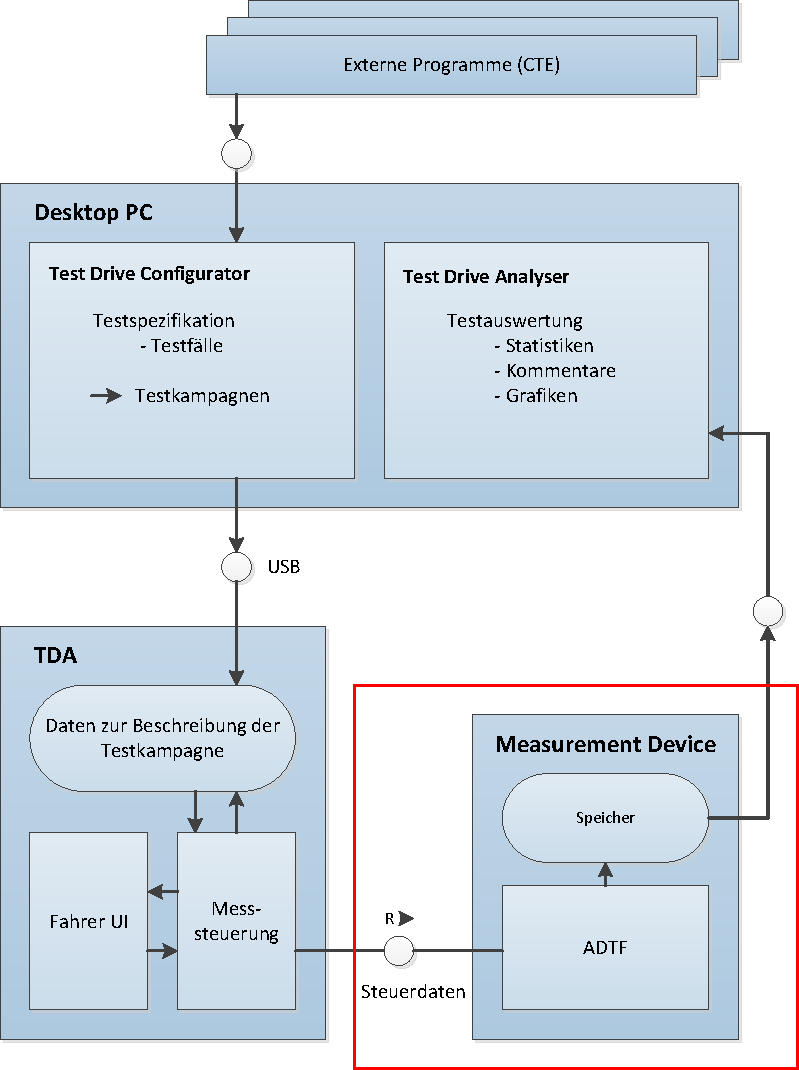
\includegraphics[scale=1.1]{Darstellungen/UebersichtKonzept}
\caption{Diagramm Komponenten des ATS}\label{pic:Blockdiagramm}
\end{center}
\end{figure}

Das Measurement Device ist im Gesamtkontext des ATS allgemein für die Aufzeichnung der Daten zuständig. Dies ist jedoch nicht die einzige Aufgabe, denn es beinhaltet folgende drei wesentliche Funktionen:
\begin{itemize}
\item{Aufzeichnung der Messdaten}
\item{Bereitstellung der Automatisierungsschnittstelle}
\item{Online-Auswertung der Messdaten}
\end{itemize}
Grundlage für die Erfüllung technischer Aufgaben ist wie in allen Fällen eine geeignete Hardwarekonfiguration. In diesem Fall besteht diese aus einem handelsüblichen Laptop auf dem die Software ADTF von Elektrobit installiert ist. Für die Wahl von ADTF als Mess-Tool im Rahmen dieses Projektes gibt es mehrere Gründe. ADTF hat sich speziell bei der Aufzeichnung von Fahrzeugdatenströmen beim Test von FAS über die Jahre etabliert. Es bietet umfangreiche Funktionen zum Aufzeichnen von Daten und ermöglicht durch die Erstellung eigener Filter eine Verarbeitung von anfallenden Daten während der Testfahrt. Somit erfüllt ADTF alle technischen Anforderungen an die Messsoftware. Des Weiteren wurde durch die vorangegangene Arbeit von Christoph Eckerlebe schon gezeigt \cite{MasterEckerlebe}, dass ADTF zur Automatisierung genutzt werden kann. Die Arbeitsergebnisse von dieser Arbeit können somit als Grundlage für die Umsetzung der Funktionen in diesem Projekt verwendet werden (s. Kap. \ref{chap:Verwendgung des TAA}).

Um die CAN-Datenströme aufzeichnen zu können, wird spezielle Hardware benötigt. Eine sehr praktische Lösung wird dafür von der Firma Vector Informatik angeboten. Das CANcase XL verfügt über zwei Sub-D Steckverbindungen, über die zwei CAN-Bus-Datenströme eines Fahrzeuges mit dem Measurement Device verbunden werden können. Dabei kann jedoch nur an einem Kanal ein Highspeed-CAN\footnote{CAN-Bus mit hoher Datenübertragungsrate} angeschlossen werden. Das CANcase XL wird via USB mit dem Laptop verbunden. Auch diese Hardware ist bereits vorhanden und kann somit sofort verwendet werden. Eine Übersicht der verwendeten Hardware bietet die Abbildung \ref{pic:Hardware}.
\begin{figure}
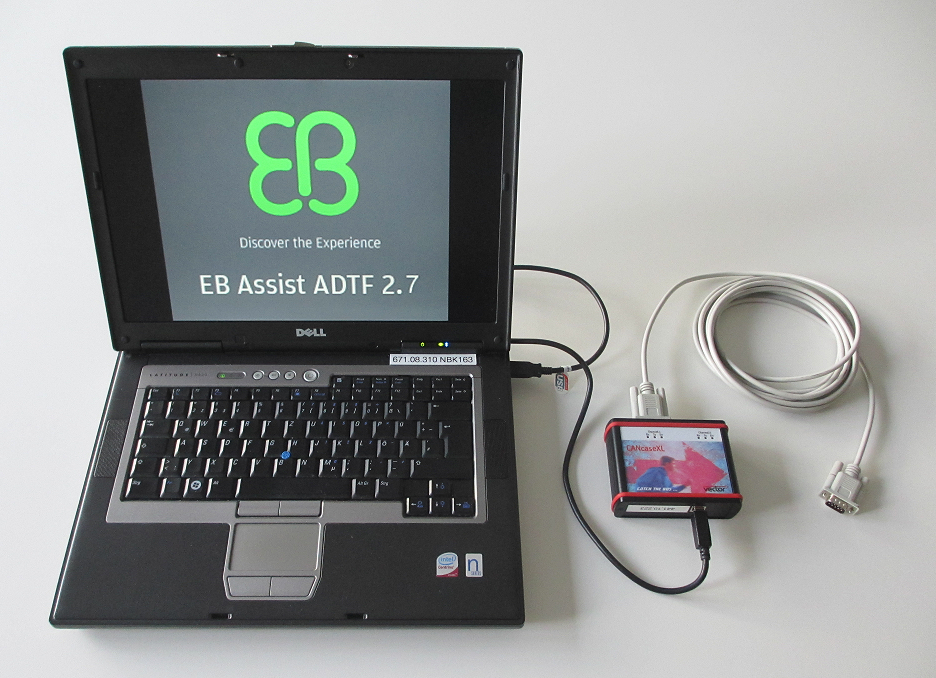
\includegraphics[width=1\linewidth]{Darstellungen/Hardware_neu}
\caption{Übersicht der Hardware für das Measurement Device}\label{pic:Hardware}
\end{figure}

Um die Messdaten während der Testfahrt aufzeichnen zu können, wird ADTF auf dem Laptop ausgeführt. In ADTF ist eine spezielle Konfiguration geladen, welche es ermöglicht über einen Filter die Daten die vom CANcase an den Laptop gesendet werden, aufzuzeichnen. Im Filtergraph befindet sich ebenso ein Filter für die Online-Auswertung, der eigens für dieses Projekt entwickelt wird. Weitere Informationen über den Aufbau des Filtergraphes und der Funktion der Online-Auswertung folgen in den Abschnitten \ref{sec:Filtergraph} und \ref{sec:Online-Auswertung2}.

Über den Python-Interpreter PSS von ADTF wird ein Python-Skript ausgeführt, welches an die Referenzimplementierung \cite{MasterEckerlebe} angelehnt ist. Es stellt das Herzstück der Steuerung von ADTF und der Kommunikation zwischen dem TDA und dem Measurement Device dar. Für die Kommunikation zwischen den beiden Systemkomponenten wird ein eigenes Protokoll auf der Grundlage der bestehenden Implementierung entwickelt, was nach den Anforderungen der Anforderungsanalyse (s. Kap. \ref{chap:Anforderungsanalyse}) entworfen wird. Zur Systemübersicht des gesamten Konzeptes des Measurement Device dient die Abbildung \ref{pic:Konzeptuebersicht}. Erklärungen zum ADTF Adapter sind unter Abschnitt \ref{sec:ADTF Adapter} zu finden.
\begin{figure}
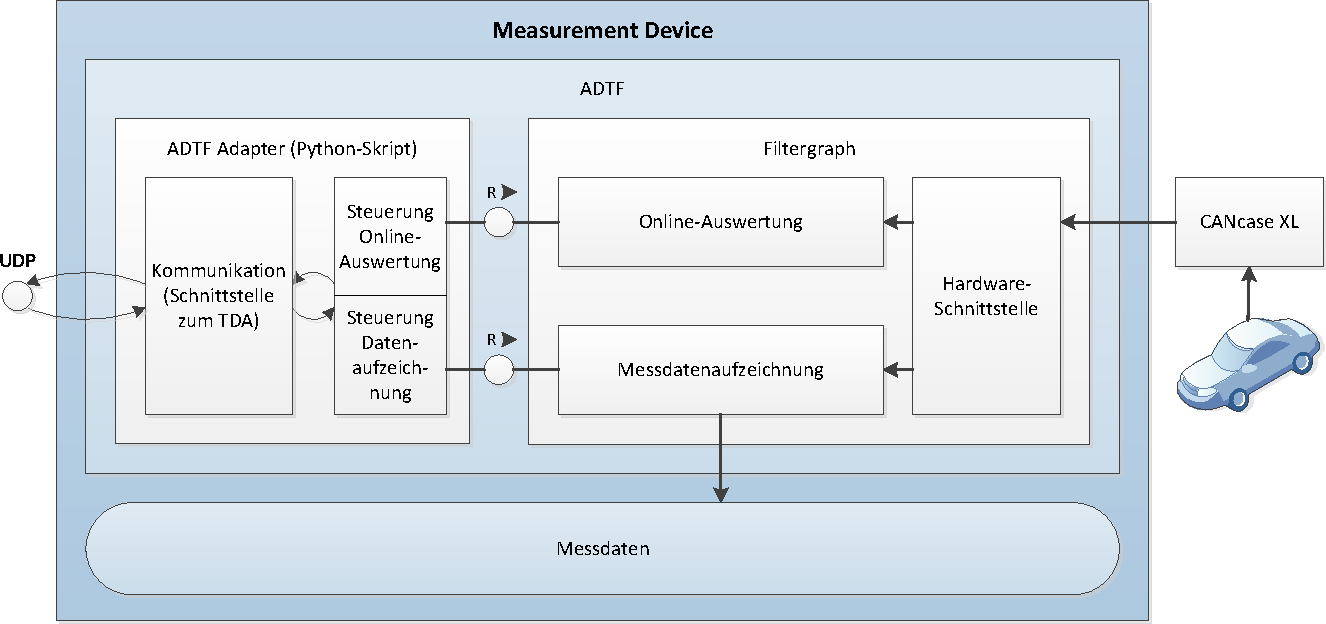
\includegraphics[width=1\linewidth]{Darstellungen/Uebersicht_Measurement-Device}
\caption{Konzeptübersicht Measurement Device}\label{pic:Konzeptuebersicht}
\end{figure}
%\newpage
\section{ADTF Adapter}\label{sec:ADTF Adapter}
Der ADTF Adapter ist in seinen Grundzügen ein Python-Skript, welches die gesamten Funktionen des Managements des Measurement Devices übernimmt. Zu den wesentlichen Aufgaben zählen dabei die Kommunikation mit dem TDA und die Steuerung von ADTF. Ein weiterer wichtiger Punkt ist jedoch auch das Fehlermanagement. Die Berücksichtigung der Anforderung bezüglich der Fehlerpotentiale hat die Implementierung einiger Mechanismen zur Fehlerdetektion und Fehlervermeidung zur Folge. Sie finden sich in den meisten Modulen wieder und sind fest in den Programmablauf eingebunden
\subsection{Kommunikationsadapter}\label{subsec:Kommunikationsadapter}
Der Kommunikationsadapter ist die Grundlage für die Kommunikation mit dem TDA und somit die Voraussetzung für die Automatisierung von ADTF. Als Erstes gilt es die Grundvoraussetzungen für die Kommunikation zu klären. Vorgabe ist es laut Anforderungsanalyse, eine kabellose Kommunikation zwischen den beiden Komponenten umzusetzen. Dazu stehen mehrere Varianten zur Verfügung, wobei sie stark an das Vorhandensein von entsprechender Hardware im jeweiligen Gerät geknüpft sind. Unter Berücksichtigung dieses Umstandes bieten sich die folgend diskutierten Kommunikationswege an.

Da es sich bei den beiden Geräten jeweils um handelsübliche Ausführungen handeln soll, kann für den Laptop und das Smartphone das Vorhandensein eines WLAN-Empfangsmoduls vorausgesetzt werden. Eine weitere fast immer verbaute Schnittstelle ist Bluetooth. Diese gilt bei Tablets als Standard, aber muss bei Laptops nicht zwingend vorhanden sein - in den meisten Fällen ist sie aber ebenso verbaut. Somit bieten sich diese beiden Kommunikationswege an.

Die erste Analyse zeigt, dass es vor allem bei Bluetooth zu Problemen bei der Programmierung kommen kann. Die normale Netzwerkverbindung über LAN/WLAN wird von Python bereits nativ unterstützt. Für die Verwendung von Bluetooth muss eine zusätzliche Programmbibliothek\footnote{eine Art Erweiterung der Programmiersprache um weitere Befehle und Funktionen} eingebunden werden. Auch bei der App-Entwicklung (TDA) kann es zu erheblichen Problemen kommen, da die Programmierung im ersten Eindruck sehr schwierig erscheint. Die Programmierung einer konventionellen Verbindung über WLAN ist demzufolge einfacher umzusetzen. Des Weiteren wurde auch bei dem von Christoph Eckerlebe bearbeiteten Projekt auf die LAN-/WLAN-Kommunikation zurückgegriffen. Die Zeitersparnis und die nicht komplett abzusehenden Risiken bei der Programmierung einer Bluetooth-Schnittstelle sind der Grund, weswegen die Entscheidung letzten Endes auf eine Kommunikation über WLAN fiel.

Nachteil der Kommunikation über WLAN ist, dass ein Access Point\footnote{Gerät, das als Schnittstelle für kabellos kommunizierende Geräte fungiert} benötigt wird. Um sich gegenseitig Nachrichten schicken zu können, müssen sowohl ADTF Adapter als auch TDA im gleichen Netz sein. Die einfachste Lösung für diese Problemstellung wäre ein Ad hoc Netzwerk\footnote{drahtloses Netzwerk zwischen zwei oder mehr Geräten}, welches vom Measurement Device (von der Windows Konfiguration des Laptops) erstellt wird. Diese Möglichkeit ist leider nicht zielführend, da sich in ersten Versuchen gezeigt hat, dass diese Umsetzung vom Tablet nicht unterstützt wird. Grund dafür sind unter anderem die Vorgaben für das Tablet, denn um möglichst hohe Kompatibilität zu ermöglichen, soll das Betriebssystem des Tablets Android sein. Android unterstützt allerdings keine Ad hoc Netzwerke, weswegen eine andere Lösung gefunden werden muss. Für den ersten Prototypen erscheint es die einfachste Lösung zu sein, mit einem handelsüblichen WLAN-Router ein WLAN-Netz aufzubauen, an dem sich Measurement Device und TDA anmelden. Der WLAN-Router stellt dann, wie in Abbildung \ref{pic:Uebersicht Kommunikation TDA Measurement Device} ersichtlich ist, den Knotenpunkt (Access Point) für die beiden Kommunikationspartner dar.

\begin{figure}[H]
\begin{center}
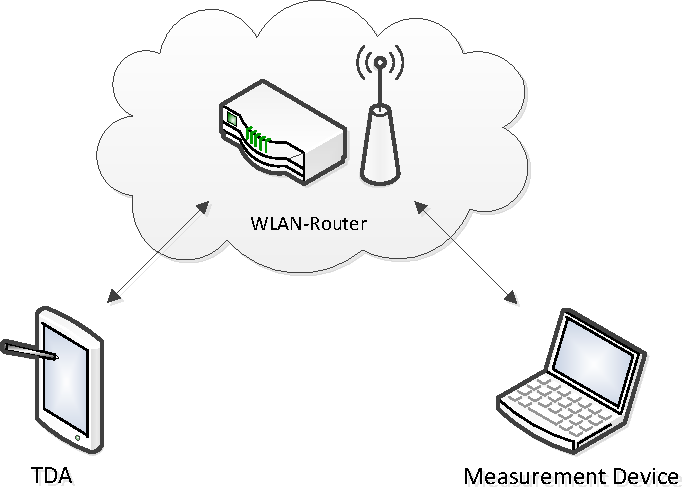
\includegraphics[scale=0.8]{Darstellungen/UebersichtKommunikationCaptureDevice2}
\caption{Übersicht der Kommunikation zwischen TDA und Measurement Device}\label{pic:Uebersicht Kommunikation TDA Measurement Device}
\end{center}
\end{figure}

\noindent Nachdem die Verbindungsart bestimmt ist, gilt es ein Protokoll für die Übertragung der Daten zu wählen. Dabei stehen die zwei bekanntesten Protokollvarianten UDP und TCP zur Wahl. Zwischen diesen beiden Protokollen bestehen grundsätzliche Unterschiede, die den Einsatz in unterschiedlichen Anwendungsfällen legitimieren. UDP ist verbindungslos und nicht zuverlässig. Bei der Verwendung des UDP-Protokolls werden Datenpakete vom Client zu einer gewählten Adresse geschickt. Es gibt dabei keinerlei Kontrollmechanismen, ob diese Netzwerkadresse besteht, ob das Paket ankommt, ob es korrekt übertragen wurde oder mehrere Pakete in der richtigen Reihenfolge ankommen. Dadurch ist die Verbindung zwar sehr schnell, aber es kann keine Garantie für die korrekte Übertragung gegeben werden. Im Gegensatz zu UDP ist TCP verbindungsorientiert und zuverlässig. Datenpakete werden bei TCP nicht einfach verschickt, sondern vorher wird eine Verbindung aufgebaut. Auf Basis dieser Verbindung wird dann die Kommunikation durchgeführt. TCP besitzt Mechanismen zur Fehlererkennung und -behebung (z.B. in Form einer Prüfsumme\footnote{einfacher Kontrollmechanismus zur Überprüfung der Datenkonsistenz}). Bei erkannten Fehlern können einzelne Pakete neu angefordert werden. Durch diese Mechanismen ist TCP zwar langsamer als UDP, aber dafür sicherer.

Für die Kommunikation zwischen dem Measurement Device und dem TDA ist keine besonders hohe Geschwindigkeit nötig. Für die Rückmeldungen der Online-Auswertung ist eine relativ hohe Latenzzeit akzeptabel, da letzten Endes der Fahrer auf diese Meldung reagieren muss und somit die menschliche Verzögerungszeit, welche sich im Zehntelsekundenbereich befindet, ausschlaggebend ist. Auch die Aufforderungen zum Steuern der Messung sind nicht zeitkritisch, da es in der Regel bei der Datenauswertung nicht auf Bruchteile von Sekunden am Anfang und am Ende der Messdatenaufzeichnung ankommt. Es ist eher untypisch, dass zu messende Ereignisse in der gleichen Sekunde geschehen, in der der Fahrer die Messung startet. Im Gegensatz dazu ist es aber durchaus nicht zu vernachlässigen, ob die Datenpakete richtig übertragen werden. Bei falsch übertragenen Datenpaketen könnten Weiterschaltbedingungen falsch interpretiert werden und somit die gesamte Messung unbrauchbar werden. Aus diesen Gründen wird das TCP-Protokoll für die Verbindung gewählt.

Dem TCP-Protokoll liegt das Client-Server-Modell zugrunde, was eingangs dieser Arbeit bereits ausreichend erläutert wurde (s. Kap. \ref{subsec:Client-Server-Modell}). Für die spätere Implementierung muss noch entschieden werden, welcher der beiden Teilnehmer die Rolle des Servers und welcher die Rolle des Clients übernimmt, da dies über die Programmierung des entsprechenden Knotens entscheidet. Grundsätzlich können bei einer TCP-Verbindung sowohl der Server als auch der Client Daten senden und empfangen. Der Unterschied liegt jedoch darin, dass der Server einen entsprechenden Port öffnen muss und somit den Dienst zur Verfügung stellen muss. Anschließend wartet der Server auf eingehende Verbindungen. Der Client hingegen muss die IP-Adresse und die Portnummer des Servers kennen, um sich mit ihm zu verbinden. Der Server ist somit ein statischer Punkt in der Netzwerkkommunikation.

Grundsätzlich wären im vorliegenden Anwendungsfall beide Möglichkeiten denkbar, so dass der ADTF Adapter und der TDA sowohl Client oder Server sein könnten. Sinnvoll erscheint es allerdings, den ADTF Adapter als Server auszuführen und für den TDA die Rolle des Clients festzulegen. Diese Belegung erscheint wegen der grundsätzlichen Definition eines Servers sinnvoll. Im Client-Server-Modell bietet der Server einen Dienst an, der vom Client in Anspruch genommen wird. Im Kontext des ATS bietet das Measurement Device Dienste für den TDA an. Das Measurement Device ist fest mit dem Fahrzeug verbunden und stellt einen statischen Zugangspunkt für Anfragen dar. Der TDA hingegen ist wesentlich mobiler und auf die Bedienung durch den Testfahrer zugeschnitten. 

Der ADTF Adapter generiert somit zum Systemstart einen Server und wartet dann auf eingehende Verbindungsanfragen. Der Testfahrer kann somit das Fahrzeug mit dem TDA betreten und seine gewünschte Testfahrt starten. Der TDA verbindet sich dann mit dem Server. Die Architektur des Kommunikationssystems zwischen TDA und Measurement Device ist in der Darstellung \ref{pic:Uebersicht Kommunikation} veranschaulicht. 
\begin{figure}
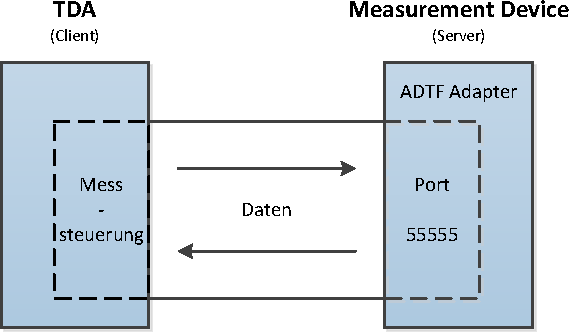
\includegraphics[width=1\linewidth]{Darstellungen/UebersichtKommunikationCaptureDevice}
\caption{Übersicht der Kommunikation zwischen Measurement Device und TDA}\label{pic:Uebersicht Kommunikation}
\end{figure}
Für die Kommunikation muss im Vorfeld ein Port festgelegt werden. Über diesen Port ist der entsprechende Dienst verfügbar. Die Portnummer ist eine ganze Zahl, die zwischen 0 und 65535 liegt. In diesem Zahlenbereich sollte jedoch nicht willkürlich eine Nummer gewählt werden, da dies zu Konflikten mit anderen Programmen und Protokollen, die auf Netzwerkkommunikation zurückgreifen, führen könnte. Dazu wurde der gesamte Zahlenraum in drei Bereiche aufgeteilt, welche der folgenden Tabelle zu entnehmen sind. Die Festlegung der Ports wird durch die Zusammenarbeit 	der IANA\footnote{IANA - \textbf{I}nternet \textbf{A}ssigned \textbf{N}umbers \textbf{A}uthority - Unterorganisation der Internet Corporation for Assigned Names and Numbers (ICANN), die sich mit der Festlegung der Portnummern befasst} und der IETF\footnote{IETF - \textbf{I}nternet \textbf{E}ngineering \textbf{T}ask \textbf{F}orce - Organisation die sich mit der technischen Entwicklung des Internets befasst} durchgeführt \cite{WikipediaPort}.
\begin{figure}[H]
\begin{center}
\begin{tabular}{|c|c|c|}
\hline
Portnummern & Bezeichnung & Beschreibung \\
\hline\hline
0 - 1023 & System Ports & durch das System verwendete Ports(neue\\&&Zuordnungen hier nur unter Beteiligung der IETF)\\
1024 - 49151 & User Ports & per Antrag festlegbare Ports (hier keine\\&&Beteiligung der IETF nötig)\\
49152 - 65535 & Dynamic Ports & Bereich zur freien Verfügung\\
\hline
\end{tabular}
\caption{Übersicht der Portnummern \cite{WikipediaPort}\cite{IETFRFC6335}}\label{tab:Uebersicht der Portnummern}
\end{center}
\end{figure}
\noindent Laut Tabelle (s. Abb. \ref{tab:Uebersicht der Portnummern}) sollte somit eine Portnummer im Bereich der Dynamic Ports gewählt werden. Die Auswahl in diesem Bereich kann jedoch willkürlich erfolgen. Die Wahl fällt dabei auf die Portnummer 55555, da diese bereits bei dem von Christoph Eckerlebe erstellten UDP-Adapter verwendet wurde.

Für die Programmierung wird die Socket-API von Python verwendet. Über diese API kann relativ einfach und zügig eine Netzwerkkommunikation aufgebaut werden.

\subsection{ADTF Steuerung}\label{subsec:ADTF Steuerung}
Hauptaufgabe des ADTF Adapters ist es, ADTF von au\ss en steuerbar zu machen. Diese Steuerung soll in den Testablauf integriert werden. Dazu schickt der TDA dem Measurement Device TCP-Nachrichten mit den kodierten Befehlen. Im Python-Skript (ADTF Adapter) werden diese Nachrichten dekodiert und die entsprechenden Befehle für ADTF generiert. Um ADTF zu steuern, wird der Python Support von ADTF (PSS) verwendet. Dieser wurde im Grundlagenkapitel bereits erläutert (s. Kap. \ref{subsec:Pythonschnittstelle}). Durch Import des ADTF Package über die Codezeile
\begin{quote}
\verb|import ADTF|
\end{quote}
ist es möglich, im Python-Skript Methoden aufzurufen, die direkten Einfluss auf die Steuerung von ADTF nehmen können.
Um die geforderten Funktionen der Anforderungsanalyse zu erfüllen, werden die folgenden Methoden genutzt.
\\[0.5cm]
\textbf{info(string)}
\\Mit dieser Funktion kann an der Konsole von ADTF eine Zeichenkette übergeben werden. Diese wird dann sofort in der Konsole auf der ADTF-Oberfläche angezeigt. Diese Funktion dient somit vor allem bei der Implementierung des Python-Skriptes als Hilfe, da mit ihr relativ leicht Zwischenergebnisse angezeigt werden können. Das Debugging wird damit erheblich vereinfacht.
\\[0.5cm]
\textbf{load\_configuration(systemxmlfile)}
\\Dieser Befehl dient zum Laden einer Konfigurationsdatei. In der Konfigurationsdatei ist der Aufbau des Filtergraphes hinterlegt sowie sämtliche Einstellungen am Projekt (z.B. Parameter der Filter oder Werte globaler Parameter). Als Parameter wird der Pfad zur entsprechenden Konfigurationsdatei angegeben.
\\[0.5cm]
\textbf{start()}
\\Diese Methode startet eine geladene Konfiguration. Der Start einer Konfiguration muss nicht den Start einer Aufzeichnung bedeuten. Durch den Startbefehl werden alle Filter in der aktuellen Konfiguration in den aktiven Status versetzt.
\\[0.5cm]
\textbf{stop()}
\\Mit Hilfe dieser Methode ist es möglich eine aktive (vorher durch den Befehl "`start()"' gestartet) Konfiguration wieder anzuhalten. Sie bleibt jedoch weiterhin geladen und kann durch einen Startbefehl wieder neu gestartet werden.
\\[0.5cm]
\textbf{start\_recording(recorderid=0,filename=}\verb|""|\textbf{,shortdesc=}\verb|""|\textbf{,longdesc=}\verb|""|\textbf{)}
\\Über diesen Befehl kann die Aufnahme in ADTF gestartet werden. Dazu muss ein Harddisk Recorder im Filtergraph vorhanden sein. Jeder dieser Recorder besitzt eine eigene RecorderID, welche diesen identifiziert. Über den ersten Parameter der Funktion wird der Startbefehl also an eine genau definierte Instanz des Recorders geschickt. Mit dem folgenden Parameter kann der Dateiname festgelegt werden, unter dem die aufgenommenen Daten gespeichert werden sollen. Die beiden darauf folgenden Parameter dienen der Beschreibung der aufgenommenen Daten. Es gibt dabei eine kurze und eine lange Beschreibung. Wichtig für die korrekte Arbeitsweise, die Aufnahme erst zu starten, nachdem die Konfiguration gestartet wurde, ist die Eigenschaft eines Harddisk Recorders "`start\_on\_startup"'. Diese muss auf "`false"' gesetzt sein, da sonst die Aufnahme sofort nach dem Start der Konfiguration beginnt.
\\[0.5cm]
\textbf{stop\_recording(recorderid=0,filename=}\verb|""|\textbf{,shortdesc=}\verb|""|\textbf{,longdesc=}\verb|""|\textbf{)}
\\Diese Funktion dient dazu, eine Aufnahme zu stoppen, ohne die gesamte Konfiguration stoppen zu müssen. Der Parameter für den Dateinamen besitzt nicht immer volle Verwendung. Wurde beim Start einer Messung bereits ein Dateiname vergeben, so kann beim Stoppen dieser Messung kein neuer Name verwendet werden. Wird jedoch trotzdem ein anderer Dateiname beim Stoppen übergeben, so wird der Befehl von ADTF abgeändert. Anders verhält es sich mit den Beschreibungen der Datei. Beim Start übergebene Werte werden zwar gespeichert, wenn beim Stopp keine weiteren übergeben werden, aber wird beim Stoppen auch eine Zeichenkette übergeben, so wird der vorherige Text überschrieben.
\\[0.5cm]
\textbf{filter\_send\_command(filterinstancename,command)}
\\Mit Hilfe dieser Methode ist es möglich, Filtern ein Kommando zu übersenden. Dieses Kommando ist in XML-Form\footnote{XML - \textbf{Ex}tensible \textbf{M}arkup \textbf{L}anguage - Auszeichnungssprache zur strukturierten Darstellung von Datensätzen} und startet eine Methode im Filter mit entsprechenden Übergabeparametern. Diese Funktion soll später dazu genutzt werden, dem Filter für die Online-Auswertung die erforderlichen Befehle zu übergeben.
\\[0.5cm]
\textbf{get\_runlevel()}
\\Diese Funktion dient dazu, den aktuellen Status der Konfiguration in ADTF festzustellen. Der Rückgabewert dieser Funktion gibt Auskunft darüber, in welchem Zustand sich ADTF im Allgemeinen befindet. Daraus lassen sich Antworten auf Anfragen, ob eine Konfiguration noch geladen ist, oder wegen eines Fehlers unterbrochen wurde, generieren.
\subsection{Kommunikationsprotokoll}\label{subsec:Kommunikationsprotokoll}
Wesentlicher Bestandteil einer Kommunikation zwischen zwei Systemkomponenten ist das Kommunikationsprotokoll. In diesem muss die gesamte Funktionalität abgebildet sein bzw. es muss alle Funktionen unterstützen. Zu diesem Zwecke wurde die Protokollstruktur der Referenzimplementierung \cite{MasterEckerlebe} erweitert. Da die Kommunikation bidirektional abläuft, muss für beide Richtungen ein entsprechendes Konzept erstellt werden, da sich die Inhalte und Aufgaben der Nachrichten unterscheiden. Das Protokoll wurde in Zusammenarbeit mit David Klowersa erstellt, der das Grundkonzept des ATS entworfen hat und die Implementierung der App für das Tablet durchführt.

Für die allgemeine Struktur des Protokolls erscheint es sinnvoll, ein Protokoll festzulegen, was für die Kommunikation in beide Richtungen verwendet werden kann. Dies dient der Einsparung von Umsetzungsaufwand, da die allgemeinen Funktionen zum Generieren und Auflösen der Nachrichten gleich bleiben. Der Unterschied liegt dann nur in der Festlegung der Message IDs und der jeweiligen Bedeutung der Messages. Bei der Kommunikation vom TDA zum ADTF Adapter kommt es überwiegend zur Erteilung von Arbeitsaufträgen für das Measurement Device. Die Kommunikation vom Measurement Device zum TDA dient hingegen eher der Beantwortung von Aufträgen oder Anfragen des TDA.
\begin{figure}[H]
\begin{center}
\begin{tabular}{|c||*{5}{c|}}
\hline
Name & Versionsnr. & Lfd. Nummer & Message ID & Message Size & Message \\
\hline
Grö\ss e & 1 & 1 & 1 & 2 & variabel \\
in Byte & & & & & \\
\hline
Datentyp & byte & byte & byte & ushort & byte array \\
\hline
%\multicolumn{3}{c|}{} & \multicolumn{2}{c|}{Header} & Body
\end{tabular}
\caption{Kommunikationsprotokoll TDA zu ADTF Adapter}\label{tab:Kommunikationsprotokoll TDA zu ADTF Adapter}
\end{center}
\end{figure}
\noindent Der Übersicht über das Protokoll dient die Tabelle in Abbildung \ref{tab:Kommunikationsprotokoll TDA zu ADTF Adapter}. Das Protokoll besteht aus fünf Feldern, die jeweils ihre Bedeutung für die Gesamtfunktion besitzen. Die Versionsnummer dient zur einfachen Erweiterung bzw. Anpassung des Protokolls für sich verändernde Anforderungen. Die momentane Funktionalität des Protokolls wird mit der Protokollversion 1 festgelegt. An dieser Stelle können später aber auch andere Werte stehen, welche dann bei der entsprechenden Auswertung der Nachrichten zur Unterscheidung genutzt werden können.

Durch die laufende Nummer, die jede Anfrage erhält, kann der ADTF Adapter gezielt auf Anfragen antworten. Dazu speichert der TDA die Information, auf welchen Auftrag (gekennzeichnet durch die laufende Nummer) er noch eine Antwort erhält. Da der TDA den Auftrag erstellt hat, kennt er die Bedingungen und den Inhalt der Aufforderung, wodurch Informationslast beim Rücksenden gespart werden kann. Beim Zurücksenden kann der ADTF Adapter sich direkt auf eine Auftragsnummer beziehen, und mitteilen, ob dieser Auftrag erfolgreich war, oder es einen Fehler gab. Die laufenden Nummern werden im Bereich von 1 bis 65535 aufsteigend vergeben. Prinzipiell kann davon ausgegangen werden, dass ein Testfall aus wesentlich weniger als den maximalen 65535 Aufträgen für den ADTF Adapter besteht, weswegen die Möglichkeit eines Überlaufs ignoriert werden kann.

Die Message ID gibt darüber Auskunft, welchem Zweck die Nachricht dient (s. Abb. \ref{tab:Bedeutung der Message ID}). Dabei findet eine Grobeinteilung nach drei Arten von Aufträgen statt. Die genauen Anweisungen werden durch weitere kodierte Identifikationsnummern in der Message festgelegt. Die Message ID dient somit vor allem der Klärung des Aufbaus der Message. Eine 1 bedeutet in diesem Fall, dass die Nachricht zum Funktionscheck der Komponenten des Measurement Devices dient oder eine Initialisierung vorgenommen werden soll. Die 2 ist festgelegt für allgemeine Steueraufträge von ADTF bzw. der Messung (z.B. Konfiguration laden, Messung starten/stoppen). Mit der 3 wird ein Auftrag für die Online-Auswertung gekennzeichnet.
\begin{figure}[H]
\begin{center}
\begin{tabular}{|c|c|}
\hline
Message ID & Bedeutung \\
\hline
\hline
 1 & Initialisierung, Funktionscheck der Komponenten \\
\hline
 2 & Steuerung von ADTF \\
\hline
 3 & Aufträge für Online-Auswertung \\
\hline
\end{tabular}
\caption{Bedeutung der Message ID}\label{tab:Bedeutung der Message ID}
\end{center}
\end{figure}
\noindent Das folgende Feld dient der sicheren Auswertung beim Empfang der Daten. Über die Message Size erhält das interpretierende Modul die Information, wie lang die eigentliche Message ist. Kommen mehrere Nachrichten hintereinander an und werden nicht einzeln ausgelesen, so werden diese geschlossen hintereinander ausgelesen. Durch die Angabe der Größe der Message kann trotzdem eine eindeutige Trennung der Nachrichten vorgenommen werden.

Im Message Feld befindet sich der eigentliche Informationsgehalt der Nachricht. Ab\-hängig von der Message ID unterscheidet sich der Aufbau der Message. Das erste Feld einer jeden Message besteht unabhängig von der Message ID aus einer Befehls ID, welche den genauen Befehl definiert. Der Aufbau einer Message in Abhängigkeit von der Message ID wird in Abbildung \ref{tab:Aufbau der Message TDA zu ADTF Adapter} dargestellt und folgend näher erläutert. Die Parameter besitzen, anders als alle anderen Felder der Message, keine feste Länge. Daher ist ein Trennzeichen erforderlich. Durch das Trennzeichen können die einzelnen Felder bei der Auswertung unterschieden werden. Als Trennzeichen wird das NULL-Byte\footnote{Variable vom Typ Byte mit dem Zahlenwert 0} gewählt, da die Parameter nur aus Daten vom Typ String bestehen. Für die Darstellung von Buchstaben, Zahlen und Sonderzeichen wird niemals das NULL-Byte verwendet, weswegen dieses als Trennzeichen verwendet werden kann (die Erklärung liegt in der ASCII-Kodierung \cite{WikipediaASCII}).
\begin{figure}[H]
\begin{center}
\begin{tabular}{|c|l|*{3}{c|}}
\hline
Message & Befehls ID & Parameter1 & Parameter2 & Parameter3 \\
ID & & & & \\
\hline
\hline
 & 1 - Kommunikation & - & - & - \\
 & noch intakt & & & \\
1 & 2 - Konfiguration & - & - & - \\
 & läuft noch & & & \\
 & 3 - Onlineaus- & String CAN & - & - \\
 & wertung möglich & Bezeichner & & \\
\hline
 & 1 - Konfiguration & String Pfad& String Pfad & - \\
 & laden & Konfiguration & Aufnahmen & \\
 & 2 - Konfiguration & - & - & - \\
 & schlie\ss en & & & \\
2 & 3 - Kommentar & String Kommentar & - & - \\
 & hinzufügen &  & & \\
 & 4 - Aufnahme starten & String Dateiname & String Kurz- & String Lang- \\
 & &  & beschreibung & beschreibung\\
 & 5 - Aufnahme stoppen & String Dateiname & String Kurz- & String Lang- \\
 & &  & beschreibung & beschreibung \\
 & 6 - Adapter stoppen & - & - & - \\
\hline
 & 1 - Werte überwachen & String auszu- & - & - \\
3 &  & wertende Klausel & & \\
 & 2 - Bedingung prüfen & String auszu- & - & - \\
 & & wertende Klausel & & \\ 
 & 3 - Bedingung prüfen & String auszu- & - & - \\
 & und Werte überwachen & wertende Klausel & & \\
\hline
\end{tabular}
\caption{Aufbau der Message von TDA zu ADTF Adapter}\label{tab:Aufbau der Message TDA zu ADTF Adapter}
\end{center}
\end{figure}
\noindent Wie bereits erwähnt wurde, dient eine Nachricht mit der Message ID 1 zum Funktionscheck oder der Initialisierung. Es sind hierbei 3 Möglichkeiten vorgesehen. Mit der ersten Möglichkeit kann überprüft werden, ob die Kommunikation noch intakt ist. Diese Nachricht besitzt prinzipiell keinen wirklichen Informationsgehalt und wird einzig dafür verwendet, den gesamten Kommunikationsweg einmal durchlaufen zu lassen. Eine entsprechende Anfrage wird vom ADTF Adapter nur quittiert. Wird dann eine Antwort vom ADTF Adapter im TDA detektiert, gilt die Kommunikation als intakt.

Durch eine andere Befehls ID kann sich der TDA bestätigen lassen, dass die Konfiguration noch aktiv ist. Dazu wird vom ADTF Adapter nur der aktuelle Systemzustand (runlevel) ausgelesen. Zeigt dieser Zustand an, dass die Konfiguration geladen ist, und läuft (runlevel 5), so wird diese Anfrage positiv quittiert. Andernfalls erfolgt eine Fehlermeldung mit entsprechender Ausgabe auf dem Tablet.

Die dritte Möglichkeit dient zur Überprüfung, ob eine Online-Auswertung mit der aktuellen Konfiguration möglich ist. Während eines Testfalls sollen mehrere CAN-Signale auf bestimmte Schwellwerte untersucht werden. Dazu benötigt das Measurement Device die Informationen, welche Nachrichten untersucht werden sollen. Um den CAN-Datenstrom verarbeiten zu können, wird das dbc-File benötigt. Liegt von diesem nicht die richtige Version auf dem Measurement Device vor, so kann die Auswertung nicht durchgeführt werden. Um eine falsche oder nicht vorhandene Dateiversion während der Laufzeit auszuschließen, muss dies zum Messstart überprüft werden. Dazu wird mit dieser Nachricht eine Liste in Form einer Zeichenkette mit den entsprechenden Bezeichnern der benötigten CAN Daten gesendet. Anschließend muss überprüft werden, ob diese Bezeichner in dem dbc-File zu finden sind. Sind alle geforderten Bezeichner in der Datei auffindbar, kann davon ausgegangen werden, dass es sich um die richtige Datei handelt.

Message ID 2 ist vorgesehen für die Steuerung von ADTF. Dazu gibt es die Möglichkeit eine vorher erstellte Konfiguration für ADTF zu laden. Um die entsprechende XML-Datei auszuwählen, wird in einem Parameter der Dateipfad der Datei übergeben. Vom ADTF Adapter wird aus dieser Anfrage der nötige Befehl generiert, um über die Python-Schnittstelle die gewählte Konfiguration zu laden. Das Laden einer Konfiguration geht immer dem Aufzeichnen von Messdaten voraus. Deswegen kann beim Laden der Konfiguration ebenfalls durch einen Parameter der Pfad für die Aufnahmen festgelegt werden. Erstellte Messungen werden dann mit ihrem Dateinamen im gewählten Ordner abgelegt. Ebenso, wie der TDA eine Konfiguration laden kann, besitzt er auch die Möglichkeit, diese wieder zu schließen. Das Schließen der aktiven Konfiguration erfordert keinen Parameter.

Aus der Anforderungsanalyse geht hervor, dass ein entscheidender Punkt die Kommentierung der Messung ist. Um ein durchgängiges Kommentierungskonzept zu unterstützen, gibt es die Möglichkeit, Kommentare in das Mess-File einzufügen. Das genaue Konzept für die Kommentierung und Dokumentierung der Messdaten ist dem Kapitel \ref{sec:Testkampagnenmanagement2} zu entnehmen.

Zwei der wichtigsten Funktionen stellt das Starten und Stoppen einer Messung durch den ADTF Adapter dar. Diese beiden Funktionen besitzen jeweils drei Parameter, da die Funktionen des Python Support von ADTF jeweils mit einem Wert für den Dateinamen, einer kurzen und einer langen Beschreibung für das Mess-File aufgerufen werden können. Wichtig zu wissen ist hierbei, dass die Zeichenketten, die für den Start der Messung übertragen werden, zwischengespeichert werden und zusammen mit allen anderen Kommentaren zum Abschluss der Messung in das Mess-File geschrieben werden. Prinzipiell muss der Dateiname nicht bei Start und bei Beendigung der Messung als Parameter verwendet werden, aber es dient der besseren Referenzierung, und unterstützt die Eindeutigkeit des Befehls, eine Datei zu schließen. Übergibt man beim Schließen (Beenden der Messung) des Mess-Files nicht den entsprechenden Dateinamen, so wird die Zuweisung automatisch von einer Systemkomponente von ADTF übernommen. Dies führte jedoch in Ausnahmefällen zu Fehlern, welche bei der automatisierten Nutzung vermieden werden sollen.

Mit Hilfe der letzten unterstützten Funktion ist es möglich, den Adapter, der von ADTF ausgeführt wird, anzuhalten. Vom Adapter werden Kommunikationsverbindungen zum TDA und zum Online-Auswertungs-Filter aufgebaut. Solche Verbindungen müssen nachdem sie nicht mehr verwendet werden, geschlossen werden. Werden die Sockets nicht ordnungsgemä\ss\ geschlossen, kommt es zu Fehlermeldungen, die zwar die Funktion der Messaufzeichnung nicht beeinflussen, aber für die Bedienung des Systems als unangenehm einzustufen sind.

Mit der letzten Message ID können Befehle für die Online-Auswertung definiert werden. Da es aktuell für die Online-Auswertung drei verschiedene Modi gibt, erscheint es sinnvoll, jedem dieser Modi eine eigene Befehls ID zuzuweisen. Alle drei Modi überprüfen eine vorher definierte Bedingung\footnote{in diesem Fall eine Verknüpfung mehrerer Bedingungen}. Der Unterschied liegt jedoch in der Art der Rück\-mel\-dung vom ADTF Adapter zum TDA. Beim Überwachen von bestimmten Werten (Modus 1), erwartet der TDA eine andauernde und periodische Antwort auf eine Anfrage, da bestimmte Werte überwacht und auf dem Tablet dargestellt werden sollen. Dazu werden die Messwerte in kurzen Abständen an den TDA geschickt. Im zweiten Modus wird eine Weiterschaltbedingung für den Ablauf des Testfalls an die Online-Auswertung übergeben. Wird die entsprechende Bedingung erfüllt, wird eine einmalige Bestätigung an den TDA verschickt, der daraufhin die Fortführung des Testfalls einleitet. Der dritte und letzte Modus ist eine Verknüpfung von den beiden vorher genannten Modi. Während eine bestimmte Klausel so wie eine Weiterschaltbedingung ausgewertet wird, werden Messdaten zu bestimmten CAN Daten ausgelesen und an den TDA gesendet. Zur genaueren Definition des Funktionsumfangs der Online-Auswertung dient Kapitel \ref{sec:Online-Auswertung2}.

Um auf Anfragen des TDA reagieren zu können, benötigt auch der ADTF Adapter ein entsprechendes Protokoll und Festlegungen, die die Kommunikation regeln. Der grundsätzliche Aufbau ist dabei, wie im Vorfeld schon angesprochen wurde, identisch und der Abbildung \ref{tab:Kommunikationsprotokoll TDA zu ADTF Adapter} zu entnehmen. Die beiden Protokolle unterscheiden sich hauptsächlich in den Bedeutungen der Werte, die in den Feldern Message ID und der Message selbst zu finden sind. Des Weiteren gibt es noch einen Unterschied in Bezug auf die Aussagekraft der laufenden Nummer.

Hauptaufgabe der Kommunikation vom ADTF Adapter zum TDA ist die Antwort auf gestellte Aufträge. Für Nachrichten solchen Charakters wird der Wert 2 für die Message ID festgelegt. Anhand der laufenden Nummer, die der laufenden Nummer des Auftrages vom TDA entspricht, kann der TDA den Auftrag identifizieren und daraus resultierende Schlüsse für den weiteren Programmablauf ziehen. Die laufende Nummer wird somit nicht neu durch Inkrementierung generiert, sondern entsprechende Werte übernommen. 

Der ADTF Adapter soll allerdings nicht nur auf Anfragen antworten, sondern auch teilweise eigene Nachrichten generieren. Es wäre beispielsweise denkbar, dass während der Messung ein Systemfehler in ADTF auftritt, welcher die Messung unterbricht. In solchen Fällen soll der ADTF Adapter eine Fehlermeldung an den TDA senden. Dazu wird die Message ID 1 verwendet. Diese speziellen Fälle haben natürlich im Gegensatz zu Anfragen vom TDA keine laufende Auftragsnummer, auf die sich die Nachricht beziehen kann. Zu diesem Zweck wird für die laufende Nummer der Wert 0 frei gehalten. Wird also am TDA eine Nachricht mit der laufenden Nummer 0 empfangen, so ist ein Systemfehler im Measurement Device aufgetreten. In diesem Fall kann noch eine Fehlerausgabe auf dem Bildschirm des Tablets durchgeführt werden.
\begin{figure}[H]
\begin{center}
\begin{tabular}{|c||*{3}{c|}}
\hline
Message ID & 1 & \multicolumn{2}{c|}{2} \\
\hline
Inhalt der& Parameter1 & Befehls ID & Parameter1 \\
Message & & &\\
\hline
Aufbau & String & 0 - keine Fehler & String Antwort \\
 & Fehlerausgabe & & auf Analyseaufträge \\
 & & 1 - Fehler & String Fehlerausgabe \\
 & & aufgetreten & \\
\hline
%\multicolumn{3}{c|}{} & \multicolumn{2}{c|}{Header} & Body
\end{tabular}
\caption{Aufbau der Message von ADTF Adapter zu TDA}\label{tab:Aufbau der Message von ADTF Adapter zu TDA}
\end{center}
\end{figure}
\noindent Im Gegensatz zum Protokoll zum ADTF Adapter, ist der Aufbau der Message des Protokolls zum TDA wesentlich einfacher aufgebaut. Soll ein Systemfehler mitgeteilt werden (Message ID 1), so besitzt diese Nachricht nur noch einen Übergabewert für einen Fehlertext, der auf dem Tablet ausgegeben werden kann. Wird mit der Message ID 2 auf einen Auftrag geantwortet, so gibt es nur die Möglichkeit, dass die erfolgreiche Ausführung des Auftrages quittiert wird (Befehls ID 0), oder die Mitteilung, dass bei der Ausführung ein Fehler aufgetreten ist (Befehls ID 1). Ist bei einem Auftrag vom TDA ein Fehler in ADTF bzw. im Measurement Device aufgetreten, so wird dafür ein entsprechender, möglichst aussagekräftiger Fehlertext generiert und dem TDA übersendet. Der TDA muss diesen Fehlertext dann nur noch ausgeben und benötigt keine weiteren Informationen zur Art des Fehlers. Die Generierung des Fehlertextes soll es erlauben, mehrsprachige Texte zu erzeugen. Dies erhöht die Komfortabilität der Nutzung des TDA.

Bei Antworten auf Aufträge für die Online-Auswertung werden mit dem Parameter1 noch weitere Daten übertragen. Wurde eine Online-Auswertung zur Überprüfung einer Weiterschaltbedingung angefordert, so wird bei Erreichen der Bedingung eine passende Antwort gesendet. Durch die Message ID 2 wird eine Antwort auf eine entsprechende Auftragsnummer (deren Wert in einem vorderen Feld der Nachricht angegeben wird) angezeigt. Der Parameter1 kann dann den Wert 1 oder 2 haben, wobei eine 1 eine nicht durchgeführte Auswertung und die 2 das Erreichen der geforderten Bedingung anzeigt.

Wird eine Online-Auswertung in Auftrag gegeben, bei der es sich um die Überwachung von Werten handelt, so werden diese Messwerte an den TDA gesendet. Dazu wird eine Antwort auf die entsprechende Auftragsnummer mit der Message ID 2 generiert. Über die Befehls ID 0 wird dann mitgeteilt, dass keine Fehler im Programmablauf aufgetreten sind. Der Inhalt von Parameter1 trägt dann die Informationen der Messwerte. Diese Übertragung der Messwerte hat eine besondere Form, da weitere Informationen neben den reinen Messwerten übertragen werden müssen. Diese Informationen geben darüber Aufschluss, von welchem Datentyp die Messwerte sind und wie der Status der Analyse der Messwerte auf ihre Schwellwerte ist. Es werden somit alle für die Entschlüsselung und Darstellung der Messwerte notwendigen Informationen übermittelt. Der genaue Aufbau der Datenpakete gehört allerdings nicht zum Konzept des Measurement Devices, da der ADTF Adapter nur für die Weiterleitung der Daten vom Filter an den TDA zuständig ist. Die Daten bekommt der ADTF Adapter in der entsprechenden Form vom Filter.
\section{Filtergraph}\label{sec:Filtergraph}
Um mit ADTF Daten aufnehmen zu können, wird eine passende Konfiguration benötigt. Eine Konfiguration ist prinzipiell eine XML-Datei, in der die gesamte Konfiguration von ADTF gespeichert ist. Eine Konfiguration besteht im Kern aus Filtern, die Daten empfangen, senden und verarbeiten können. Zur Erstellung von solchen Konfigurationen kann der Configuration Editor von ADTF benutzt werden. Dieser bietet eine graphische Oberfläche und dient der schnellen Erstellung von Konfigurationen.

Um mit dem Measurement Device des ATS die volle Funktionalität zu erreichen, ist ein entsprechender Filtergraph unabdingbar. Die allgemeine Steuerung von ADTF wird vom ADTF Adapter (Python-Skript) übernommen, aber die tatsächliche Aufnahme von Datenströmen wird über die in ADTF geladene Konfiguration durchgeführt. Der Filtergraph muss eine Schnittstelle zur an den Laptop angeschlossenen Mess-Hardware (CANcase XL) bieten. Über einen speziell für die Vector-Hardware entworfenen Filter, der zusammen mit den allgemeinen Treibern der Vector-Hardware konfiguriert werden muss, kann der Datenstrom, der durch das CANcase detektiert wird, in ADTF importiert werden. Über den Ausgangspin des entsprechenden Filters wird der Datenstrom für weitere Filter nutzbar gemacht. Dieser Datenstrom soll als erste Vorgabe auf dem Measurement Device gespeichert werden. Dazu wird ein weiterer Filter in Form eines "`Harddisk Recorders"' benötigt.

Die zweite Aufgabe ist die sofortige Auswertung der Daten nach speziellen Kriterien. Die Online-Auswertung erfolgt in einem selbst entwickelten Filtermodul, welches den am CANcase anliegenden Datenstrom übergeben bekommt. Vom ADTF Adapter bekommt dieses Filter die für die Online-Auswertung benötigten Daten. Das Konzept für die Online-Auswertung wird in Abschnitt \ref{sec:Online-Auswertung2} genauer erläutert. Zur Veranschaulichung der Filterstruktur dient Abbildung \ref{pic:Filtergraph in ADTF}. Sie stellt den kompletten für die Messwerterfassung und -auswertung nötigen Filtergraphen dar.
\begin{figure}
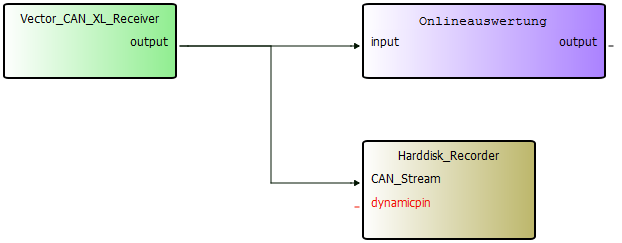
\includegraphics[width=1\linewidth]{Darstellungen/Filtergraph}
\caption{Filtergraph in ADTF}\label{pic:Filtergraph in ADTF}
\end{figure}
\section{Testkampagnenmanagement}\label{sec:Testkampagnenmanagement2}
Um die aufgezeichneten Messdaten später eindeutig zuordnen zu können, müssen Mechanismen festgelegt werden. Grundlage für die Umsetzung der geforderten Funktionen ist das Dateiformat von Messungen in ADTF. ADTF bietet durch das Dateiformat und die Python-API (PSS) bereits ausreichend viele Möglichkeiten, die für das Testkampagnenmanagement verwendet werden können. Ein Mess-File (.dat-File) besteht nicht nur aus den aufgenommenen Messwerten, sondern auch aus einer kurzen und einer langen Beschreibung. Diese beiden Textfelder können genutzt werden, um Kommentare zu den Messungen zu speichern. Auch der Dateiname kann frei gewählt werden.

Durch die Funktionen der Python-API, wird beim Start einer Messung deren Dateiname festgelegt. Bei Beendigung der Messung werden die Textfelder für die kurze und lange Beschreibung übergeben und zusammen mit den Messwerten in einer Datei gespeichert. Es ist jedoch nicht möglich, die Beschreibungsfelder des dat-files während der Messung zu ändern. Dadurch müssen alle während der Testfahrt erstellten Kommentare vorgehalten werden, um zum Abschluss der Messung geschlossen übergeben werden zu können.

Mit dem Speichern der Kommentare ist eine wichtige Frage verbunden, die vor allem in Bezug auf das Auftreten von Systemfehlern von Bedeutung ist. Der Speicherort der Kommentare bestimmt maßgeblich, das mögliche Verhalten bei Fehlerfällen. Tritt ein Systemfehler am Measurement Device auf, gibt es relativ wenig Möglichkeiten, diese abzufangen, da die Messdaten höchstwahrscheinlich gar nicht gespeichert oder aufgenommen werden und somit durch Fehlermechanismen kaum zu retten sind. Anders sieht es jedoch bei Systemfehlern des Tablets aus. Fällt das Tablet aus, kann das Measurement Device, und damit die Messung, nicht mehr gesteuert werden. Um bereits gesammelte Messwerte nicht zu verlieren, wird die Messung eigenständig vom ADTF Adapter beendet, wenn dieser den Ausfall des TDAs vermeldet. Die Detektion des Ausfalls des TDAs wird über eine zyklisch generierte "`Alive-Anfrage"' des TDAs umgesetzt. Innerhalb eines festen Zeitfensters muss eine Kommunikation zwischen TDA und ADTF Adapter stattfinden. Zwischen zwei am ADTF Adapter angekommenen Paketen darf nur eine bestimmte maximale Zeit vergangen sein. Da es vorkommen kann, dass bei einer längeren Messung der ADTF Adapter über längere Zeit keine Anfragen vom TDA erhält, gibt es sogenannte "`Alive-Anfragen"'. Dies sind im Grunde leere Datenpakete (besitzen also keinen Informationsgehalt in der Message selbst), welche durch den ADTF Adapter positiv beantwortet werden. Gibt es innerhalb einer festgelegten Zeit keine "`Alive-Anfrage"' oder normale Steueranfrage, kann der ADTF Adapter von einem Systemfehler des TDAs ausgehen.

Würden bei einem solchen Fehlerfall die Kommentare zur Messung auf dem Tablet gespeichert sein, könnten diese nicht mehr im Mess-File gespeichert werden. Um diese Kommentare im Fehlerfall nicht zu verlieren, werden sie auf dem Measurement Device gespeichert. Wird ein neuer Kommentar mit dem TDA erstellt, wird eine entsprechende Nachricht generiert und an den ADTF Adapter gesendet. Dieser hängt den neuen Kommentar an eine Liste von bereits gespeicherten Kommentaren, die bei Beendigung der Messung als lange Beschreibung gespeichert werden sollen, an. Zusätzlich wird in der Beschreibung der Messdaten ein Kommentar hinterlegt, welches anzeigt, dass die Messung aufgrund eines Systemfehlers eigenständig abgebrochen wurde.

Der Dateiname kann vor Beginn der Messaufzeichnung festgelegt werden und wird vom TDA beim Startbefehl einer Messung übergeben. Bereits bei der Erstellung der Testspezifikation werden eindeutige Dateinamen festgelegt, welche eine spätere Auswertung und Zuordnung der Daten ermöglichen. Wenn eine Messung aufgrund eines Fehlers wiederholt werden muss, wird als Dateiname für die Messdaten ein Name gewählt (vom TDA an den ADTF Adapter übergeben), unter dem theoretisch auf der Festplatte bereits eine Messung gespeichert ist. Da keine Daten überschrieben werden sollen, und um Fehler zu vermeiden, wird in diesem Fall der Dateiname passend um eine angehängte, inkrementierte Zahl erweitert. Diese Zahl ist zweistellig, womit eine Messung maximal 100 Mal durchgeführt werden kann. Dieser Wert wurde vorerst frei gewählt und unterliegt keinen besonderen Bestimmungen.
\section{Online-Auswertung}\label{sec:Online-Auswertung2}
Wie bereits des Öfteren erwähnt wurde, ist eine Grundfunktion des ATS die zeitnahe Auswertung der Fahrzeugdatenströme. Diese Datenströme müssen sozusagen "`online"' ausgewertet werden, um dem Testfahrer eindeutig mitzuteilen, dass bestimmte Bedingungen für das Voranschreiten des Testfalls erfüllt wurden. Außerdem soll es die Möglichkeit geben, sich auf dem Tablet bestimmte Messwerte anzeigen zu lassen, um diese einfacher während der Testfahrt überwachen zu können. Da die Messdaten mit Hilfe des Measurement Devices und ADTF aufgezeichnet werden, erscheint es logisch diese Auswertelogik in diesem Kontext umzusetzen. ADTF bietet hierfür die Möglichkeit eigene Filter zu programmieren. Diese können Datenströme empfangen, weiterleiten, interpretieren oder auch verändern. Um die geforderten Funktionen umzusetzen und den Testfahrer bestens zu unterstützen, soll in der ADTF-Konfiguration ein Filter vorhanden sein, welcher die Fahrzeugdatenströme empfängt, Teile dieser Messdaten auswertet und sofern dies gefordert ist, weiterleitet. Dieser Filter muss eigens für dieses Projekt entwickelt werden. Die Planung und Erstellung dieses Filters ist nicht Teil dieser Bachelorarbeit, sondern wird im Rahmen einer anderen Abschlussarbeit durchgeführt. Das grundlegende Konzept, wie die Funktionen dieses Filters verwendet werden, ist jedoch Teil des Gesamtkonzeptes des Measurement Devices und somit auch Teil dieser Abschlussarbeit. Das Konzept zur Anbindung der Online-Auswertung wird in Zusammenarbeit mit Daniel Tarrach erstellt, der für die Entwicklung und Umsetzung der Online-Auswertung zuständig ist.

Das Filter für die Online-Auswertung der CAN-Daten ist Teil der grundlegenden Konfiguration von ADTF, welche vor allem zur Aufzeichnung der Messdaten dient (s. Abb. \ref{pic:Filtergraph in ADTF}). Über den Eingangs-Pin werden die Daten des CAN-Bus, welche durch das CANcase XL detektiert werden, empfangen. Im Inneren des Filters werden die auszuwertenden Nachrichten auf bestimmte Bedingungen geprüft. Diese Überprüfungen sind sehr dynamisch, da sich die auszuwertenden Bedingungen stark unterscheiden. Verschiedene Testkampagnen dienen zum Test verschiedener FAS und verlangen die Überprüfung völlig unterschiedlicher Messwerte. Die zu überwachenden CAN-Signale differieren somit allein aufgrund der zu testenden FAS. Zum anderen können sich die Bedingungen während eines Testfalls stark unterscheiden. Die Geschwindigkeit könnte beispielsweise zum Anfang eines Testfalls auf eine Geschwindigkeit von 50 km/h geprüft werden und im Laufe des Versuchs auf 80 km/h geprüft werden. Somit muss das Filter von außen steuerbar sein. Das Filter selbst bietet somit Grundfunktionen zur Überwachung von CAN-Signalen, welche durch Übergabe entsprechender Parameter auf den entsprechenden Anwendungsfall zugeschnitten werden.

Ebenso, wie es für die Kommunikation zwischen TDA und ADTF Adapter nach einem Kommunikationskonzept verlangt, muss es auch ein Konzept für die Kommunikation des ADTF Adapters mit dem Filter zur Online-Auswertung geben. Zwar sind beide Komponenten Teil der Instanz der Software ADTF, aber die Kommunikation zwischen ihnen ist nicht ohne Weiteres umzusetzen. Der ADTF Adapter ist ein Python-Skript, welches durch einen Python Interpreter in ADTF ausgeführt wird und durch eine Bibliothek begrenzte Zugriffs- und Steuermöglichkeiten für ADTF bietet. 

Um mit dem Filter kommunizieren zu können, gibt es eine entsprechende Funktion des PSS, welche es erlaubt dem Filter ein Kommando zu senden. Dieses Kommando ist ein Funktionsaufruf in XML-Form. In dem Kommando sind der Name der aufzurufenden Funktion, sowie die zu übergebenden Parameter hinterlegt. Über dieses Kommando ist es möglich eine im Filter selbst programmierte Funktion mit Parametern aufzurufen und somit dem Filter neue Aufträge zu erteilen und ihn in einen bestimmten Überwachungsmodus zu versetzen. Der Kommunikationsweg vom ADTF Adapter zum Filter ist somit relativ leicht umzusetzen. Schwieriger ist jedoch die Kommunikation in die andere Richtung umzusetzen. Das Filter selbst kann zwar auf nahezu alle Funktionen von ADTF zugreifen, jedoch nicht auf ein Python-Skript, was ausgeführt wird. Eine Erklärung dafür ist vielleicht darin zu sehen, dass ADTF erst im Nachhinein um die Scripting-Schnittstelle erweitert wurde und diese somit nicht so tief im System verankert ist, wie es andere Komponenten sind.

Aus der Untersuchung von Beispielprojekten im Zuge der anderen Abschlussarbeit ergab sich, dass es nur zwei Möglichkeiten der Kommunikation mit einem Python-Skript gibt. Die erste Variante hängt mit den Eigenschaften eines jeden Filters zusammen. Jeder Filter besitzt Eigenschaften (sog. "`Properties"'), welche sowohl Zahlenwerte als auch Zeichenketten darstellen können. Die Anzahl und die Art und Weise der Eigenschaften ist bei der Programmierung eines Filters frei wählbar. Über die Funktionen des PSS ist es möglich diese Properties zu verändern und auszulesen. Das Filter muss dafür allerdings angehalten werden. Genau dies stellt ein gro\ss es Problem dar, da der PSS keine Funktionen bietet, einen Filter in einen anderen Systemzustand zu überführen. Der Zustand eines Filters kann nur durch die globale Veränderung des "`Runlevels"' erfolgen. Die Veränderung des Runlevels auf einen Wert, bei dem das Filter seinen Wert ändern könnte, würde allerdings auch alle anderen Filter der Konfiguration anhalten. Die Folge wäre das sofortige Beenden einer Messung, welche gleichzeitig zur Auswertung der Daten erfolgt. Dieser Sachverhalt ist für die gesamte Funktion des Measurement Devices nicht tragbar, da somit ständig die Messungen angehalten werden würden. Diese wieder zu starten und fortzuführen ist in ADTF nicht möglich, da bestehende Mess-Files nicht erneut geöffnet und fortgesetzt werden können. Diese Möglichkeit der Steuerung des Filters ist somit nicht zielführend und wird verworfen.

Die andere Möglichkeit setzt, ähnlich wie die Kommunikation zwischen TDA und ADTF Adapter, auf ein Protokoll der Netzwerkkommunikation. Es handelt sich dabei um die Kommunikation über UDP. In Abbildung \ref{pic:Kommunikationskonzept mit der Onlineanalyse} ist eine Übersicht über das Kommunikationskonzept zwischen dem ADTF Adapter und dem Online-Analyse-Filter dargestellt. Ausgehend von einem Beispielprojekt von ADTF wird in einem Filter ein UDP Client aufgebaut, der Daten an einen entsprechenden Server sendet. Dieser Server wird durch den ADTF Adapter zur Verfügung gestellt. Somit ist es möglich dem ADTF Adapter Informationen zur aktuellen Online-Auswertung zu senden. Die Daten werden dann vom ADTF Adapter empfangen und in einer entsprechenden Form an den TDA weitergeleitet. Die Daten, die vom Filter gesendet werden, hängen vom gewählten Modus ab. Während in einem Modus der Filter eine Bedingung überprüft und dann nur eine Meldung bei Erfüllung der Bedingung versendet, werden in anderen Modi bestimmte Messwerte überwacht und dazu die tatsächlichen Messwerte weitergeleitet.
\begin{figure}
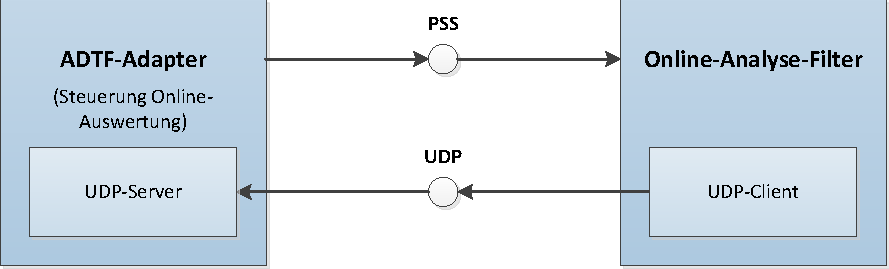
\includegraphics[width=1\linewidth]{Darstellungen/Konzept-Adapter-Filter}
\caption{Kommunikationskonzept zwischen ADTF Adapter und Filter}\label{pic:Kommunikationskonzept mit der Onlineanalyse}
\end{figure}
Da die Kommunikation mit dem Filter in beide Richtungen erfolgen soll, muss es für beide Richtungen Konventionen geben. Aus der Anforderungsanalyse ergibt sich, dass das Filter zwei Modi unterstützen soll. Zum einen die Überprüfung einer bestimmten Bedingung\footnote{bestehend aus der logischen Verknüpfung von bestimmten Prüfphrasen von CAN-Signalen} sowie dem zeitnahen darstellen von Messwerten, welche auch auf bestimmte Schwellen überprüft werden sollen. Im ersten Fall sollen bestimmte Messwerte zur Kontrolle für den Testfahrer auf dem Tablet-Bildschirm dargestellt werden. Diese Messwerte sollen auch auf Bedingungen bzw. Schwellwerte überprüft werden. Der Unterschied zum vorher genannten Modus ist jedoch, dass die einzelnen Messwerte und ihre Bedingungen nicht gegeneinander geprüft werden. Es gibt somit keine logische Verknüpfung von Bedingungen. Dieser Modus soll dem Testfahrer Arbeit bei einfachen Testfahrten abnehmen, bei dem genau definierte Manöver abgefahren werden. Bei diesen Testfahrten sollen bestimmte Messwerte definierte Grenzwerte nicht unter- und/oder überschreiten. Auf dem Tablet werden dem Fahrer die aktuellen Messwerte angezeigt und bei Verstoß gegen die Grenzwerte soll eine farbliche Markierung den Fahrer darüber informieren.

Im zweiten Modus bekommt das Filter die entsprechende Phrase zur Überprüfung übergeben. Anschließend werden die CAN-Signale auf diese Bedingung geprüft. Ist die Bedingung erfüllt, wird eine Nachricht generiert, welche an den ADTF Adapter gesendet wird und das Erfüllen der gewählten Bedingung anzeigt. Der ADTF Adapter schickt seinerseits nach dieser Nachricht eine Meldung an den TDA, der auf die Bestätigung dieser Bedingung wartet. Auf eine Anfrage zur Überprüfung vom TDA zum ADTF Adapter werden somit vom ADTF Adapter zwei Antworten generiert. Zuerst wird der Eingang des Auftrages quittiert und nachdem die Bedingung erfüllt wurde, wird die entsprechende Nachricht generiert, welche das Erreichen der zu untersuchenden Bedingung anzeigt. Der TDA bekommt somit in Summe zwei Nachrichten, wobei nur beim Erhalt der zweiten Nachricht, das Erfüllen der zu untersuchenden Bedingung bekundet wird. Diese Art der Analyse ist im Protokoll durch den Wert 2 repräsentiert.

Um den Einsatzbereich des ATS zu erweitern soll die Online-Auswertung einen weiteren Modus zur Verfügung stellen. Im dritten Modus werden die beiden anderen Modi kombiniert. Denkbar wäre ein Szenario, bei dem eine bestimmte Bedingung zum Fortführen des Testfalls erfüllt werden soll. Um diese Bedingung zu erreichen, müsste der Testfahrer eventuell einen bestimmten Zustand des Fahrzeuges erreichen. Das Erreichen dieses Zustandes kann in manchen Fällen viel "`Fingerspitzengefühl"' erfordern und vom Testfahrer verlangen, dass er bestimmte Messwerte gleichzeitig berücksichtigen muss. Um diese Fälle besser zu unterstützen, sollen die Messwerte auf dem Tablet-Bildschirm angezeigt werden. Bei Erfüllung einer geforderten Bedingung sollen jedoch noch weitere Fahrmanöver für einen Testfall durchgeführt werden. Somit gibt es auch in diesem Fall eine Art Weiterschaltbedingung, die die Fortführung der Testfahrt ermöglicht. Diese Variante der Überprüfung stellt den dritten Modus dar.

Um das Filter in den entsprechenden Modus zu versetzen wird eine Funktion des PSS verwendet. Somit ist kein gesondertes Protokoll nötig. Im Filter müssen jedoch die gesendeten Funktionsnamen unterstützt und die Verarbeitung des Funktionsaufrufs umgesetzt sein.
Für jeden der drei Modi gibt es einen eigenen Funktionsaufruf mit entsprechender Form der Parameter. Da der Funktionsaufruf in XML-Form erfolgt, sieht die Grundstruktur eines zu sendenden Kommandos wie folgt aus:
\begin{quote}
\verb|<cmd name="Funktionsname" Parameter1="..." Parameter2...>|
\end{quote}
Die Parameter beschreiben, welche CAN-Signale wie überprüft werden sollen. Diese Über\-prüfungen werden bereits mit der Testspezifikation erstellt und sind in der entsprechenden Form in den Daten für die Testkampagne hinterlegt. Die Belegung der Parameter soll an dieser Stelle jedoch nicht weiter erläutert werden, da dies für das Konzept des ADTF Adapters nicht von Belang ist. 

Für die Funktionsnamen gibt es noch einen weiteren Wert, der dazu dient, das auf dem Messrechner abgelegte dbc-File zu untersuchen und zu validieren. Am Anfang einer Messung soll zunächst geprüft werden, ob auf dem Messrechner die richtige Datei abgelegt wurde, da die Online-Auswertung der Daten mit einer falschen Datei nicht möglich ist. Die folgende Übersicht soll die verfügbaren Funktionsaufrufe auflisten (s. Abb. \ref{tab:Uebersicht der Funktionen des Filters}).
\begin{figure}[H]
\begin{center}
\begin{tabular}{|c|c|}
\hline
Funktionsname & Bedeutung \\
\hline\hline
validateDBC & Überprüfung des dbc-Files vornehmen\\
setupFilter & Prüfbedingung setzen\\
setupMonitoringFilter & Prüfbedingung setzen und Messdatenrückgabe festlegen\\
activateMonitoring & Messdatenrückgabe festlegen\\
\hline
\end{tabular}
\caption{Übersicht der Funktionen des Filters }\label{tab:Uebersicht der Funktionen des Filters}
\end{center}
\end{figure}
\noindent Das Zurücksenden von Daten vom Filter unterliegt auch strengen Regeln. Dazu wird der Aufbau der Nachrichten, in denen Messdaten oder nur einfache Bestätigungen enthalten sind, festgelegt. Der detaillierte Aufbau soll hier jedoch nicht beschrieben werden, da der Inhalt der Nachrichten für den ADTF Adapter keinen Stellenwert besitzt. Es sind lediglich Daten, die vom ADTF Adapter in der korrekten Form an den TDA weitergeleitet werden müssen\footnote{in das normale Übertragungsprotokoll eingebettet}.

Je nach gewähltem Modus unterscheiden sich die vom Filter gesendeten Daten sehr stark. Da der ADTF Adapter durch Auswertung der Anweisungen des TDA "`wei\ss "', in welchem Modus das Filter ist, kann der Adapter auf die Antworten unterschiedlich reagieren. Dies ermöglicht, dass der Aufbau der Nachrichten für jeden Modus unterschiedlich sein kann. Im ersten Feld der Nachricht befindet sich jedoch immer eine Identifikationsnummer, welche anzeigt, in welchem Modus sich das Filter befindet. Dies dient zur Kontrolle. Soll das Filter nur eine Weiterschaltbedingung überprüfen, so genügt eine kurze Rückmeldung vom Filter ohne weiteren Informationsgehalt. Eine leere Nachricht zeigt somit das Erreichen der geforderten Bedingung an. Befindet sich das Filter in einem Modus, bei dem Messwerte zurückgegeben werden sollen, folgen diese Werte mit den zur Auswertung nötigen Informationen\footnote{Angaben zur Anzahl der Messwerte und deren Datentypen ermöglichen die eindeutige Auswertung der Daten} auf die Identifikationsnummer. 
\chapter{Implementierung und Test des ADTF Adapters}\label{chap:Implementierung}
Nachdem das detaillierte Konzept für das Measurement Device erstellt wurde, kann die eigentliche Umsetzung der geforderten  Funktionen durchgeführt werden. Bevor jedoch der Quellcode generiert werden kann, muss geplant werden, wie das Konzept umgesetzt wird. Dazu müssen weitreichende Überlegungen über den Aufbau und die Struktur des Softwaremoduls angestellt werden. Im Vorfeld wird somit schon die genaue Struktur des Moduls festgelegt. Mit Hilfe von geeigneten Darstellungen, werden die Überlegungen zusammengefasst und das Grundgerüst des Quellcodes festgelegt, anhand dessen die Implementierung durchgeführt werden kann.

Zur Planung der Quellcodestruktur wird in diesem Projekt auf zwei Darstellungsformen zurückgegriffen. Bei der ersten Darstellungsform handelt es sich um das Klassendiagramm, welches über die bestehenden Klassen, Funktionen und das Gefüge zwischen den einzelnen Objekten Auskunft gibt. Um den Programmablauf besser darstellen zu können, dienen Sequenzdiagramme, welche auch den zeitlichen Ablauf näher beleuchten. Werden diese beiden Darstellungsformen kombiniert, entsteht ein schlüssiges Bild über den zu erstellenden Code.

Bei der Implementierung spielen aber auch Tests eine wichtige Rolle, da trotz eines gut ausgearbeiteten Konzeptes Fehler in der Programmierung nicht komplett auszuschließen sind. Dazu müssen nach und während der Codeerstellung die umgesetzten Funktionen getestet werden. Da in diesem Projekt auf bestehende Softwaremodule von ADTF zurückgegriffen wird (vor allem der PSS), sollen diese zunächst auf richtige Funktion überprüft werden. In der Vergangenheit zeigte sich, dass die Python Unterstützung teilweise Fehler aufwies, da Funktionen nicht wie beschrieben agierten. Um weitere Fehler auszuschließen, werden alle Funktionen des PSS, die in diesem Projekt Verwendung finden sollen, geprüft.

Im folgenden Kapitel wird das Ergebnis der Implementierung und der durchgeführten Tests vorgestellt.
\section{Test des PSS}\label{sec:Test des PSS}
Der Python Support Service von ADTF stellt ein zentrales Element im Konzept des Measurement Devices dar. Erst durch die Python-Schnittstelle ist es möglich ADTF von außen zu steuern und somit für dieses Projekt automatisieren zu können. Deswegen besitzt der Test dieses Moduls eine sehr hohe Bedeutung. Die Bedeutung ist auch dadurch zu erklären, dass in vorangegangenen Verwendungen des PSS Fehlfunktionen aufgedeckt wurden. Es handelte sich dabei allerdings um ältere Versionen von ADTF, weswegen die Vermutung sehr nahe liegt, dass die Probleme behoben wurden. Des Weiteren dient der Test auch dazu, die genaue Bedeutung der Funktionen herauszufinden. In der Dokumentation von ADTF \cite{ADTFDokuSDK}  ist die API nur sehr kurz und grob beschrieben, weswegen die tatsächliche Funktion nicht komplett in ihrer Gänze daraus hervorgeht. 

Da es sich beim PSS um ein verhältnismäßig kleines Modul handelt, kann von komplizierten und zeitaufwendigen Testläufen (wie automatisierte Tests) Abstand genommen werden. Um die Funktionen adäquat zu testen, genügt es, diese durch gezielte Aufrufe mit anschließender Untersuchung der darauf folgenden Ergebnisse zu testen. Dazu werden kleine Beispielprogramme verwendet. Aufgrund der Trivialität der erstellten Beispielprogramme werden sie an dieser Stelle nicht vorgestellt, sondern nur die Herangehensweise und die Ergebnisse der Tests präsentiert. 

Nach Möglichkeit soll jede Funktion für sich selbst getestet werden um Wechselwirkungen auszuschließen. In manchen Fällen ist dies jedoch nicht möglich, da das Ergebnis von manchen Funktionen erst nach Aufruf einer weiteren Funktion ersichtlich ist. Ein Beispiel hierfür wäre die Funktion "`set\_recording\_folder"'. Der Aufruf dieser Funktion mit einem geeigneten Parameter hinterlegt lediglich in ADTF einen Dateipfad für Messungen. Die Auswirkungen dieses Funktionsaufrufes sind erst nach dem Start einer Messung darin zu erkennen, dass die aufgenommene Datei sich in dem vorgegebenen Dateipfad befindet.

Der Test erwies sich am Ende als erfolgreich. Alle Funktionen, die Verwendung finden, funktionieren wie gefordert und können die Anforderungen aus der Anforderungsanalyse bedienen. Die genaue Funktion der Methoden ist in Kapitel \ref{subsec:ADTF Steuerung} angegeben.
\section{Struktur des Skriptes}\label{sec:Struktur des Skriptes}
Unter den Vorgaben des Entwurfs für das Measurement Device wurde der Aufbau des ADTF Adapters geplant. Die grundsätzliche Struktur des entwickelten Softwaremoduls wird anhand des Klassendiagramms (s. Abb. \ref{pic:Klassendiagramm}) vorgestellt.
\begin{figure}
\begin{center}
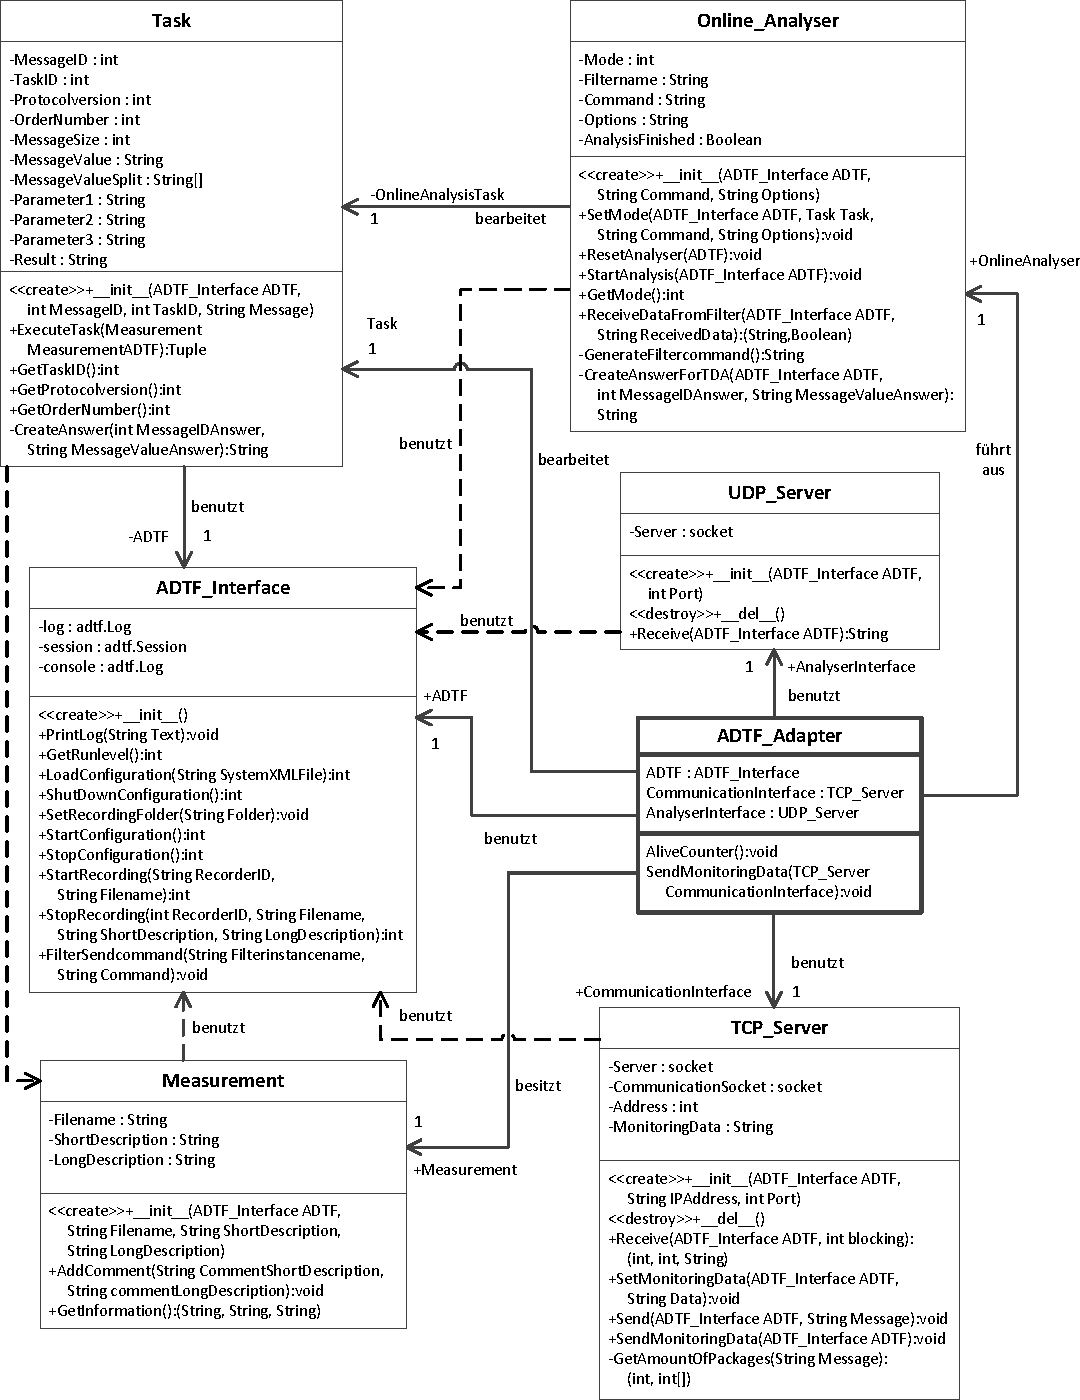
\includegraphics[scale=0.85]{Darstellungen/Klassendiagramm}
\caption{Klassendiagramm ADTF Adapter}\label{pic:Klassendiagramm}
\end{center}
\end{figure}
Im Wesentlichen besteht der ADTF Adapter aus einem Verbund von sechs Klassen und einem zentralen Skript. Das zentrale Skript ist der eigentliche ADTF Adapter, der direkt in ADTF eingebunden und interpretiert wird. Der ADTF Adapter selbst ist keine Klasse, übernimmt aber die "`Verwaltung"' der verwendeten Objekte. Zum besseren Verständnis ist der ADTF Adapter trotzdem im Klassendiagramm dargestellt und als zentrales Element durch dickere Randlinien hervorgehoben. Da der ADTF Adapter kein Objekt von einer Klasse ist, besitzt er auch keine klassischen Attribute, sondern globale Variablen. Im Klassendiagramm sind nur Variablen, die zum Verständnis der Struktur dienen, angegeben.

Die wohl wichtigste Klasse die vom ADTF Adapter verwendet wird ist die Klasse des ADTF Interfaces. Über die Methoden des ADTF Interfaces kann die Software ADTF aktiv gesteuert werden. Dazu wird, wie in Kapitel \ref{subsec:ADTF Steuerung} beschrieben ist, eine Bibliothek importiert, durch dessen Benutzung ADTF gesteuert werden kann. Um das Programm übersichtlicher und verständlicher zu halten, soll ADTF an möglichst wenigen Stellen des Quellcodes gesteuert werden. Die Steuerung soll zentral von wenigen Instanzen durchgeführt werden. Lediglich der ADTF Adapter selbst und Objekte der Klasse Task sollen auf die Steuerung von ADTF Einfluss nehmen. 

Somit besitzen Objekte der Klasse Task ein Attribut "`ADTF"', welches ihnen ermög\-licht ADTF zu steuern. Für den ersten Prototypen gibt es allerdings auch andere Probleme, die in der Planung bedacht werden müssen. Beim Entwurf eines komplett neuen Moduls hat es oft große Bedeutung, Konsolenausgaben zu generieren (z.B. für Methodenaufrufe). Erst dadurch ist es in vielen Fällen möglich, den Quellcode zu überprüfen und sicherzustellen, dass die Funktionen das gewünschte Verhalten besitzen. Die einzige Möglichkeit Konsolenausgaben anzuzeigen, ist die ADTF-Konsole zu verwenden, welche während der Laufzeit in der IDE\footnote{IDE - \textbf{I}ntegrated \textbf{D}evelopment \textbf{E}nvironment - Entwicklungsumgebung} dargestellt wird. Um eine Ausgabe auf dieser Konsole durchzuführen, wird der Zugriff auf ein Objekt der Klasse ADTF Interface benötigt. Das bedeutet, dass am Ende jedes Objekt von jeder Klasse Zugriff auf das ADTF Interface benötigt um Konsolenausgaben zu generieren. Um trotzdem diese beiden Typen von Klassen zu unterscheiden, besitzen nur solche Klassen, die ADTF steuern sollen, ein Attribut, um auf die Steuerung von ADTF zuzugreifen. 

Um trotzdem eine Konsolenausgabe durchführen zu können, werden bei Methodenaufrufen von anderen Klassen jeweils das Objekt ADTF vom Typ ADTF Interface als Parameter übergeben. Im Klassendiagramm ist dieser Unterschied an der Art der Pfeile erkennbar. Während eine Assoziation mit einem durchgezogenen Pfeil dargestellt wird, ist der Pfeil, der eine Abhängigkeitsbeziehung darstellt, gestrichelt \cite{OestereichUML}. Außerdem werden bei einer Abhängigkeitsbeziehung keine Angaben zur Multiplizität an den Enden der Verbindung vorgenommen.

Eine wesentliche Aufgabe des ADTF Adapters ist die Kommunikation mit anderen Modulen des Systems. Der wichtigste Kommunikationsweg hierbei ist der Datenaustausch mit dem TDA, da der ADTF Adapter vom TDA seine Aufträge erhält. Da die Kommunikation mit dem TCP-Protokoll über WLAN durchgeführt wird, muss die entsprechende Infrastruktur durch Quellcode zur Verfügung gestellt werden. Dazu dient die Klasse TCP Server. Mit Hilfe eines Objektes von dieser Klasse ist der ADTF Adapter in der Lage Daten vom TDA zu empfangen und seinerseits Nachrichten an den TDA zu senden.

Beim Empfang von Daten über TCP kann es dazu kommen, dass mehrere Nachrichten hintereinander gesendet werden. Wird zwischen den Nachrichten nicht die Funktion "`Receive(...)"' vom TCP-Server aufgerufen, so stehen die Nachrichten im Speicher hintereinander. Wird dann die Methode aufgerufen, werden die Nachrichten zusammen ausgelesen. Um keine Informationen zu verlieren, wird beim Empfang erkannt, wie viele Nachrichten gesendet wurden. Anschließend wird die Verarbeitung für jedes empfangene Paket durchgeführt.

Neben der Kommunikation mit dem TDA muss der ADTF Adapter aber noch die Schnittstelle zur Online-Auswertung bereitstellen. Diese wird von einem Filter in der ADTF Konfiguration durchgeführt. Um Nachrichten von dem Filter zu erhalten, stellt der ADTF Adapter einen UDP-Server zur Verfügung. Für diesen steht ebenfalls eine Klasse zur Verfügung. Mit Hilfe eines Objektes der Klasse UDP Server können Daten vom Online-Analyse-Filter empfangen werden. Die Daten werden direkt vom ADTF Adapter empfangen, indem dieser die entsprechende Methode des UDP-Servers aufruft. Die Verarbeitung der empfangenen Daten und die anschließende Generierung von Antwortnachrichten auf Aufträge für die Online-Analyse werden durch ein Objekt der Klasse Online Analyser durchgeführt.

Nachrichten die vom TDA an den Adapter gesendet werden, werden grundlegend als Auftrag angesehen. Selbst wenn es sich nur um eine Botschaft zum Überprüfen der Verbindung handelt, wird diese Anfrage als Auftrag angesehen und als solcher bearbeitet. Nach Bearbeitung muss eine Antwort generiert und gesendet werden. Für die Verarbeitung, Bearbeitung und Erstellung von Antworten auf Aufträge dient die Klasse Task. Nachdem eine Nachricht erhalten wurde, wird immer ein Task generiert. Durch Aufruf der Methode "`ExecuteTask(...)"' wird die Verarbeitung gestartet. Im Zuge der Bearbeitung des Tasks wird auch ADTF gesteuert, wenn dies für die Erfüllung des Auftrages nötig ist.

Über die Klasse Measurement werden alle für die Messung notwendige Daten gespeichert. In ADTF besitzen Messdaten zwei Kommentierungsfelder, die jeweils zum Start und zum Beenden einer Messung belegt werden können. Um Kommentare während der Durchführung der Messung zu erstellen, müssen diese bis zum Ende der Messung gespeichert werden. Durch die Methode "`AddComment(...)"' können neue Kommentare hinzugefügt werden. Zum Ende der Messung werden alle Kommentare zusammen abgerufen (als Zeichenkette) und durch den Aufruf zum Stoppen einer Messung in den Messdaten hinterlegt.
\section{Programmablauf}\label{sec:Programmablauf}
Im folgenden Abschnitt soll die Arbeitsweise des Skriptes vorgestellt werden. Zur Er\-läu\-te\-rung werden Sequenzdiagramme verwendet, welche das Verständnis erleichtern sollen. An dieser Stelle sei darauf hingewiesen, dass es wenig sinnvoll wäre, den gesamten Quellcode zu erläutern. Deswegen soll anhand von drei exemplarischen Abläufen die allgemeine Arbeitsweise vorgestellt werden. Im ersten Beispiel wird das Verhalten beim Laden einer Konfiguration beschrieben. Mit dem zweiten Beispiel wird vorgestellt, wie der Alive-Counter umgesetzt ist, durch den das Skript automatisch beendet wird, wenn die Kommunikation zum TDA über längere Zeit abgebrochen ist. Der Alive-Counter agiert nebenläufig zum Rest des Programms. Dadurch bildet sich eine spezielle Struktur aus, welche an diesem Beispiel näher erläutert werden soll. Im letzten Diagramm wird die Interaktion mit dem Filter für die Online-Auswertung und das periodische Senden von Messdaten vorgestellt.
\subsection{Konfiguration Laden}\label{subsec:Konfiguration Laden}
Das Laden einer Konfiguration steht meistens am Anfang eines Testzyklus', denn bevor Messdaten aufgezeichnet werden können, muss die entsprechende Konfiguration in ADTF geladen werden. Die Konfiguration ist zwingend erforderlich und muss auf das entsprechende Fahrzeug angepasst werden. Für den ersten Prototypen soll davon ausgegangen werden, dass die Konfigurationsdatei durch einen Ingenieur, der für die Durchführung der Tests verantwortlich ist, nach einem festgelegten Muster erstellt wird. Die Konfiguration sollte mit ADTF erstellt werden. Das Ergebnis dieses Prozesses ist eine "`XML-Datei"', welche alle Informationen der Konfiguration enthält.

Um diese Konfigurationsdatei zu laden, muss der TDA eine Nachricht nach dem vereinbarten Protokoll (s. Kap. \ref{subsec:Kommunikationsprotokoll}) erstellen und senden. Diese Nachricht beinhaltet den absoluten Dateipfad zu der Konfigurationsdatei als Parameter1 sowie den Dateipfad für zu erstellende Messdaten. Nachdem die Nachricht generiert und gesendet wurde, setzt das Sequenzdiagramm in Abbildung \ref{pic:Sequenz Load Config} ein.
\begin{figure}
\begin{center}
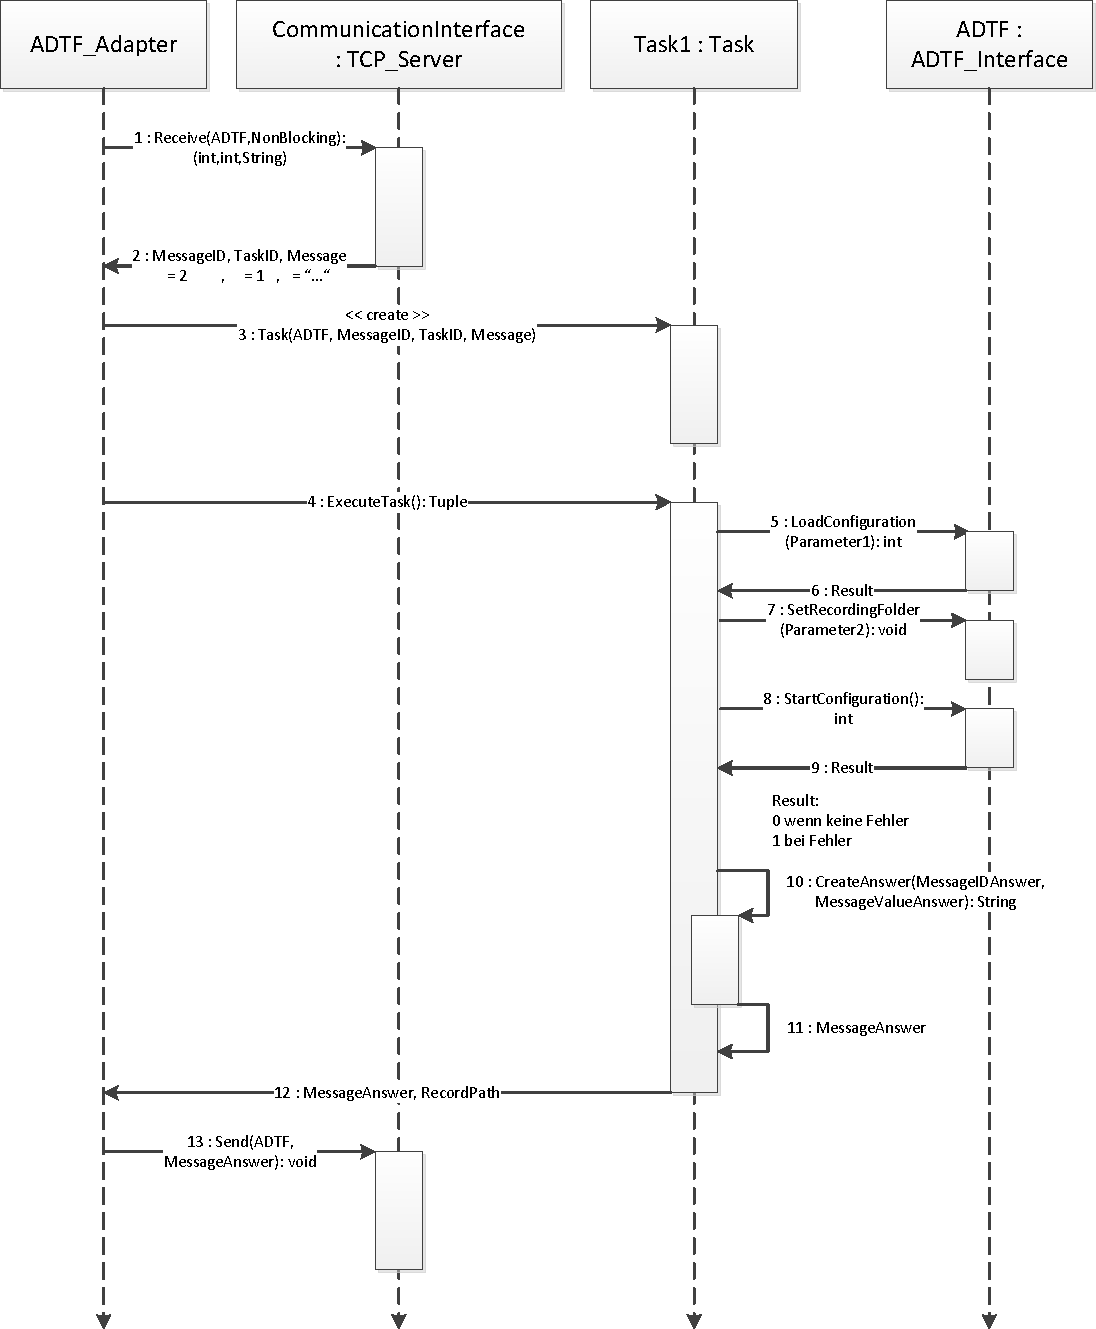
\includegraphics[scale=0.85]{Darstellungen/SequenzLoadConfig}
\caption{Sequenzdiagramm Konfiguration Laden}\label{pic:Sequenz Load Config}
\end{center}
\end{figure}
Durch den Aufruf der Funktion "`Receive(ADTF,NonBlocking)"' werden neue Nachrichten, die den TCP-Server seit dem letzten Auslesen erreicht haben, empfangen. Beim Auslesen des Sockets im Communication Interface, wird eine zusammenhängende Zeichenkette empfangen. Direkt nach dem Auslesen werden die Werte für die MessageID und die TaskID der Nachricht ermittelt. Der Rückgabewert der Methode ist ein Tuple, bestehend aus drei Variablen. Die Variablen MessageID, TaskID und Message sind Felder, die jeweils so viele Elemente besitzen, wie Pakete angekommen sind. Somit können mehrere Pakete empfangen und anschließend verarbeitet werden. In diesem Beispiel ist jedoch nur eine Nachricht mit der MessageID 2 und der TaskID 1 angekommen. Über den zweiten Parameter des Methodenaufrufs kann angegeben werden, ob der Server neue Nachrichten blockierend empfangen soll. Beim blockierenden Empfangen, wartet der Server so lange, bis eine neue Nachricht angekommen ist. Prinzipiell wäre es für die Steuerung von ADTF kein Problem den Server blockierend zu verwenden. Allerdings würde diese Betriebsart die Online-Auswertung nicht unterstützen, da in diesem Modus oft Nachrichten an den TDA gesendet werden sollen und somit neben dem Warten auf neue Aufträge andere Aktionen durchgeführt werden sollen. Um trotzdem beide Modi zu unterstützen kann der Server sowohl blockierend als auch nicht blockierend aufgerufen werden.

Der ADTF Adapter benötigt die Information, von welchem Typ eine Nachricht ist, um die entsprechende Verarbeitung der Nachricht anzuleiten. Dies kommt vor allem daher, dass mitunter Methoden verschiedener Objekte aufgerufen werden müssen, um einen Auftrag auszuführen. Beim Start einer Messung muss beispielsweise ein Objekt der Klasse Measurement erzeugt und dessen Attribute belegt werden. Des Weiteren muss der Harddisk Recorder in der ADTF-Konfiguration gestartet werden, was nur durch die Klasse Task möglich ist. Da der ADTF Adapter aufgrund seiner Aufgaben den genauen Aufbau einer Nachricht nicht "`kennen"' muss, ist es sinnvoller die Vorauswertung\footnote{Auslesen der TaskID und MessageID} kurz nach dem Empfangen der Nachricht im Communication Interface durchzuführen. Das Communication Interface "`kennt"' den genauen Aufbau einer Nachricht, weil nur so mehrere angekommene Nachrichten identifiziert und getrennt werden können. Alle weiteren wichtigen Daten sind in den Parametern der Nachricht enthalten und dürfen nicht verloren gehen. Deswegen wird die gesamte Nachricht ebenfalls zurückgegeben.

Anschlie\ss end wird ein Objekt der Klasse Task generiert. Vom Objekt Task1 wird dann die Methode "`ExecuteTask()"' aufgerufen, was die eigentliche Verarbeitung der Nachricht nach sich zieht. In dieser Klasse wird auch der restliche Inhalt der Nachricht (die Parameter) ausgelesen. Abhängig von der MessageID und der TaskID werden Prozesse angesto\ss en, die zur Erfüllung des Auftrages beitragen. In diesem Beispiel wäre das der Aufruf der Funktion "`LoadConfiguration(...)"' vom ADTF Interface mit dem Parameter1 der Nachricht. Im Parameter1 ist der absolute Dateipfad der Konfigurationsdatei angegeben. Die zweite Aktion die durchgeführt wird, ist das Festlegen des Pfades für zukünftige Aufnahmen, was auch durch den Aufruf einer Methode des ADTF Interfaces durchgeführt wird. Zum Schluss wird noch die gesamte Konfiguration von ADTF gestartet. 

Abhängig vom Erfolg der ausgeführten Methoden, wird eine Antwort für den Task generiert. Diese Antwort wird im Task1-Objekt erstellt und muss nach dem vereinbarten Protokoll aufgebaut werden. Anhand der Rückgabewerte der Methodenaufrufe des ADTF Interfaces wird erkannt, ob der Auftrag korrekt durchgeführt werden konnte. Tritt ein Fehler auf, so wird ein entsprechender Fehlertext generiert und in der Nachricht gespeichert. Somit kann für jeden erkennbaren Fehler ein entsprechender Fehlertext an den TDA gesendet werden. Durch Ausgabe des Fehlertextes, kann die Fehlersuche anschließend vereinfacht werden.

Die generierte Nachricht wird per Rückgabewert an den ADTF Adapter übergeben. Des Weiteren wird der Pfad für zukünftige Aufnahmen zurückgegeben, da dieser für die Bearbeitung der Dateinamen der Messdaten von Bedeutung ist. Diese Funktion ist zwar aktuell noch nicht gefordert, soll aber hiermit schon unterstützt werden. Durch den Parameter kann der ADTF Adapter nachvollziehen, an welchem Ort ein Mess-File abgelegt wird oder werden soll. Somit kann vorher geprüft werden, ob unter einem gewählten Dateinamen bereits Messdaten hinterlegt sind und der Name somit durch einen Zusatz erweitert werden sollte.

Nachdem der Auftrag durchgeführt wurde, muss die Antwort an den TDA weitergeleitet werden. Die fertig erstellte Nachricht wurde dem ADTF Adapter als Rückgabewert übermittelt und kann durch Aufruf der Methode "`Send(ADTF,MessageAnswer)"' des Communication Interfaces gesendet werden.
\subsection{Alive-Counter}\label{subsec:Alive-Counter}
Der Alive-Counter soll verhindern, dass Messdaten verloren gehen, wenn es im Betrieb des Tablets zu einer schwerwiegenden Störung kommt. In diesem Fall ist das Measurement Device von außen nicht mehr steuerbar, da der Kommunikationspartner fehlt. Um das Measurement Device in einem solchen Fall trotzdem in einen kontrollierten Zustand zu überführen, ist im Konzept ein Sicherheitsmechanismus vorgesehen. Nach dem Verstreichen einer gewissen Zeit ohne Anfrage des TDAs, stoppt sich der ADTF Adapter selbständig. Das Sequenzdiagramm (s. Abb. \ref{pic:Sequenz AliveCounter}) zeigt, wie dieses Modul im Programmablauf integriert ist.

Um die gewünschte Funktion zu implementieren, wurde ein zum Hauptprogramm nebenläufiger Prozess entwickelt. Der Prozess besteht aus einer Funktion, die mit einer Verzögerung von 60 Sekunden ausgeführt wird. Man spricht hier von einem Thread, der die Funktion AliveTest ausführt. Der TDA ist so eingestellt, dass er alle 30 Sekunden eine Nachricht generiert, die die Kommunikation überprüft. Der normale Programmablauf\footnote{Empfang und Verarbeitung von Nachrichten} des ADTF Adapters wird nur durchgeführt, wenn die globale Variable "`TDAisAlive"' auf True gesetzt ist. Dies signalisiert eine intakte Kommunikation. Wenn auf dem Tablet der TDA nicht mehr aktiv ist, wird die nebenläufige Funktion nach 60 Sekunden ohne Anfrage ausgeführt. Als Folge werden alle aktiven Module des ADTF Adapters gestoppt und schließlich der Adapter selbst angehalten.

Aus dem Diagramm ist zu erkennen, dass der nebenläufige Thread AliveTest vom Hauptprogramm gestoppt wird, sobald eine Nachricht vom TDA detektiert wird. Anschlie\ss end wird er wieder neu gestartet. Wird über den Aufruf der Methode "`Receive(...)"' 60 Sekunden lang keine Nachricht empfangen, wird die Funktion "`AliveTest"' aufgerufen. In ihr wird dann die Variable "`TDAisAlive"' auf False gesetzt.
\begin{figure}
\begin{center}
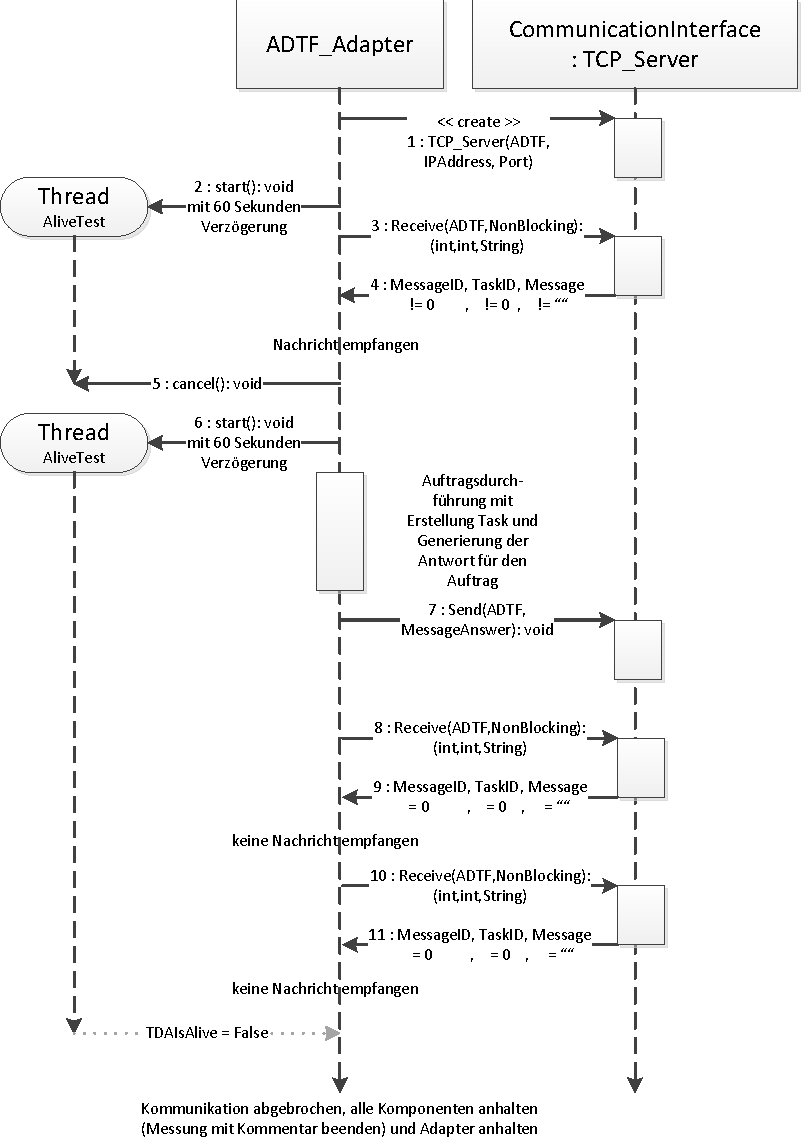
\includegraphics[scale=1.05]{Darstellungen/SequenzAliveCounter}
\caption{Sequenzdiagramm Alive-Counter}\label{pic:Sequenz AliveCounter}
\end{center}
\end{figure}
\subsection{Online-Analyse}\label{subsec:Online Analyse}
Die Verarbeitung von Anfragen zur Online-Analyse ist etwas komplexer als normale Steuerbefehle für ADTF. Zur Bearbeitung solcher Aufträge wird ein weiteres Kommunikationsinterface benötigt, da die eigentliche Auswertung der Messdaten durch ein Filter realisiert wird. Um dem Filter Aufträge zu erteilen, wird eine Methode des PSS verwendet. Um Informationen vom Filter zu erhalten, wird jedoch ein UDP-Server verwendet. Im Sequenzdiagramm in Abbildung \ref{pic:Sequenz Online-Analyse} wird der Programmablauf für das Bearbeiten einer Anfrage an den Analysefilter veranschaulicht. Im vorliegenden Beispiel bekommt das Filter den Auftrag, die Messwerte auf eine Weiterschaltbedingung hin zu überprüfen und gleichzeitig Messdaten in regelmä\ss igen Abständen zu liefern.
\begin{figure}
\begin{center}
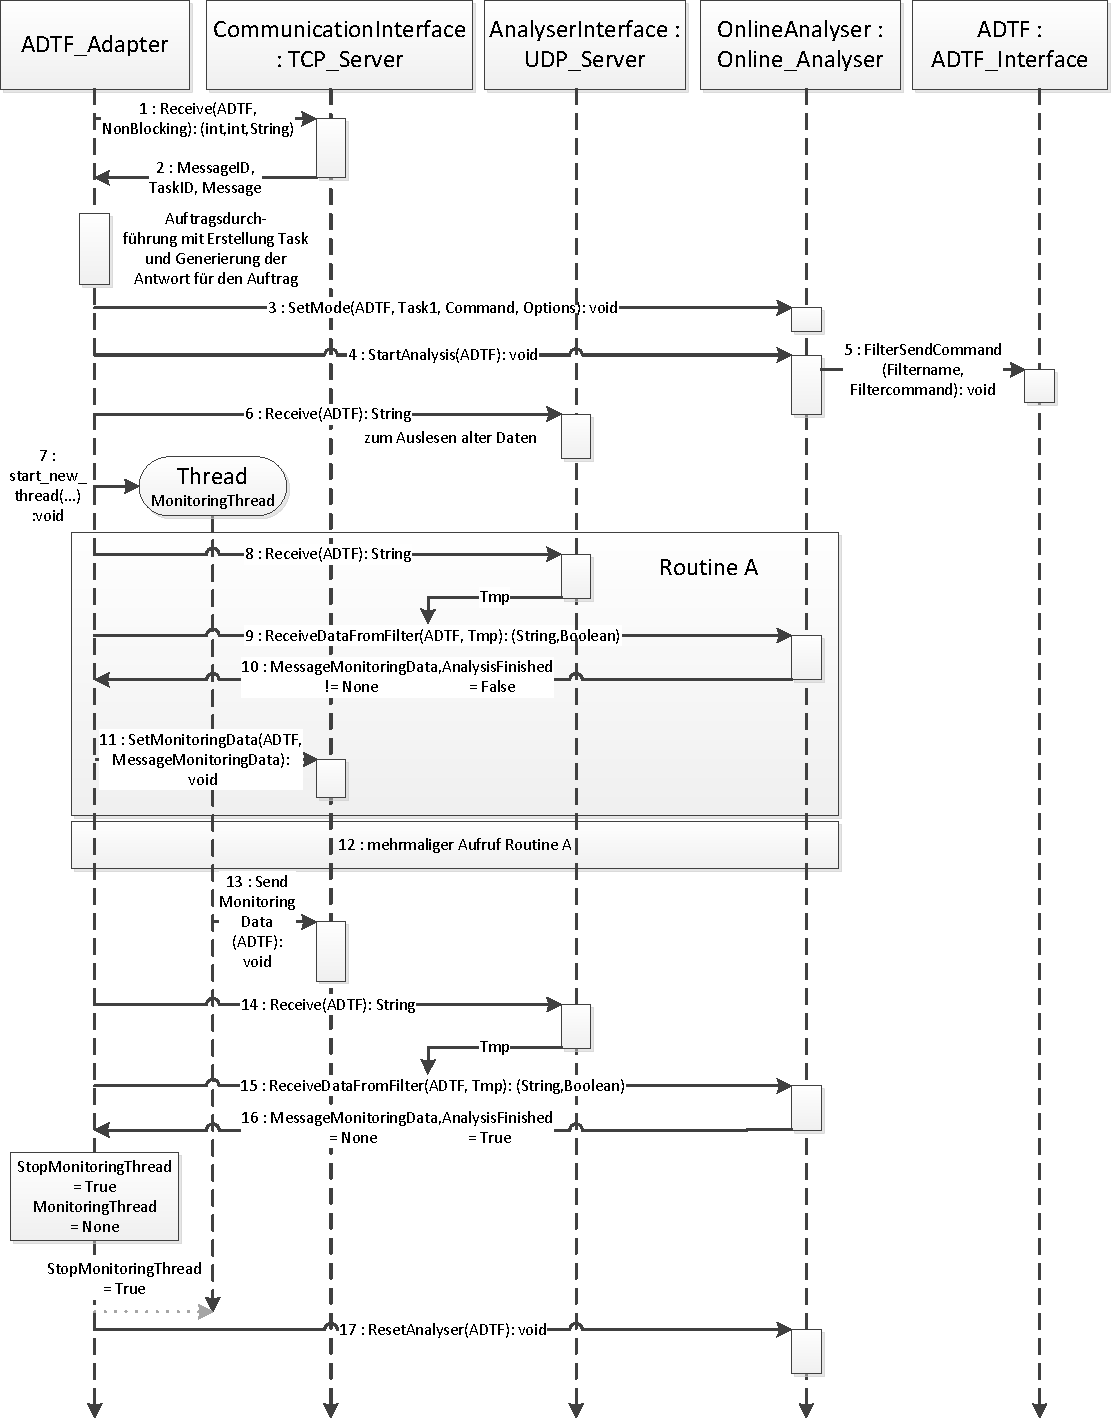
\includegraphics[scale=0.85]{Darstellungen/SequenzProofMonitoring}
\caption{Sequenzdiagramm Online-Analyse}\label{pic:Sequenz Online-Analyse}
\end{center}
\end{figure}
Der Beginn des Programmablaufs ähnelt dem Entgegennehmen eines normalen Auftrages, wie in Abschnitt \ref{subsec:Konfiguration Laden}. Es wird eine Nachricht empfangen und anschließend verarbeitet. Die Generierung eines Tasks und dessen Ausführung ist in diesem Schaubild nur verkürzt dargestellt, da eine genauere Erklärung zu diesen Abläufen dem ersten Beispiel zu entnehmen ist. Anschließend beginnt die eigentliche Verarbeitung des Auftrages.

Bevor eine Online-Auswertung beauftragt werden kann, muss das dbc-File überprüft werden. Dazu wurde im Vorfeld schon eine Nachricht gesendet, die den Filter beauftragt, das dbc-File zu überprüfen, ob alle zu analysierenden Messwerte durch diese Datei aufgelöst werden können. Dies stellt sicher, dass bei der Erstellung der Tests und der Durchführung der Tests die gleiche Datei verwendet wurde und die geforderten Messwerte somit analysiert werden können. War diese Überprüfung erfolgreich, wird ein Objekt der Klasse Online Analyser generiert, welches aber noch keine Informationen über eine anstehende Auswertung enthält. Erst nach Erhalt einer Nachricht, um eine Analyse zu starten, werden die für die Analyse notwendigen Informationen an dieses Objekt übergeben. Dabei werden über die Methode "`SetMode(...)"' die Parameter des Analysers gesetzt. Ausgehend von diesen Parametern kann durch den folgenden Befehl "`StartAnalysis(...)"' die geforderte Analyse gestartet werden. Dazu wird das Filter über den Befehl "`FilterSendCommand(...)"' des ADTF Interfaces in den gewünschten Zustand versetzt. Das Kommando wird vor dem Senden durch eine Methode des Objektes OnlineAnalyser generiert. 

Das Filter wird durch das gesendete Kommando in einen Modus überführt, der eine genau definierte Charakteristik, abhängig von der geforderten Funktion, besitzt. In diesem Fall wird das Filter ständig aktualisierte Messdaten und den aktuellen Status der zu untersuchenden Bedingung an den UDP-Server senden\footnote{in einem zusammenhängenden Datenpaket}. Die Datenpakete vom Filter haben abhängig vom gewählten Modus ein festgelegtes Format, welches dem TDA bekannt ist. Dadurch müssen die Messdaten vom ADTF Adapter nicht interpretiert werden und können fast unverändert an den TDA weitergeleitet werden. Der ADTF Adapter muss nur "`wissen"' wie sich das Filter verhalten wird.

Bevor die eigentliche Auswertung und Weiterleitung der Messdaten vom Filter beginnen kann, müssen eventuelle Datenreste aus dem Speicher gelesen werden. Dazu wird einmalig die Methode "`Receive(...)"' aufgerufen.

Das Filter sendet in unregelmä\ss igen Abständen aktualisierte Daten. Die Zeitabstände zwischen den Nachrichten hängen direkt von der Taktung der CAN Botschaften ab. Sobald sich ein zu untersuchender Wert ändert, wird ein neues Datenpaket vom Filter gesendet. Allerdings kann vorher nicht kalkuliert werden, wann neue Daten eintreffen, da dies von der Aktualisierungszeit der CAN-Signale und deren Priorität abhängt. Es ist trotzdem damit zu rechnen, dass wesentlich mehr Datensätze generiert werden, als für die Darstellung auf dem TDA notwendig sind. Die Messwerte sind als Hilfsmittel für Testfahrten gedacht, um dem Testfahrer während der Fahrt eine Rückmeldung über wichtige Messwerte zu geben. Da der Testfahrer diese Messwerte nur nebenbei beobachten kann - schlie\ss lich muss das Fahrzeug vorrangig bedient werden - wird eine Aktualisierungszeit von 0,5 Sekunden gewählt. Bei dieser Zeitspanne handelt es sich um einen aus eigenen Erfahrungen abgeschätzten Wert, der keinen wissenschaftlichen Betrachtungen unterliegt.

In diesem Zusammenhang erscheint es wenig sinnvoll, alle aktualisierten Messwerte an den TDA weiterzuleiten. Um die Kommunikationslast zu verringern, werden nur alle 0,2 Sekunden die aktuellen Messwerte weitergeleitet.  Um diese Vorgabe umzusetzen, wurde ein nebenläufiger Prozess entwickelt, der auf der Thread-Programmierung beruht. Dazu wird eine zum Hauptprogramm nebenläufige Methode aufgerufen. In diesem Thread wird eine Dauerschleife ausgeführt. Ziel dieses Threads ist es eine Taktung zum Senden der Messdaten vorzunehmen. Dazu besteht der Rumpf der Dauerschleife aus einem Funktionsaufruf, der dafür sorgt, dass die Durchführung des nebenläufigen Prozesses eine vorgegebene Zeit wartet. Diese Zeitspanne beträgt, wie soeben benannt wurde, 0,2 Sekunden. Nach Ablauf dieser Zeit wird eine Methode des CommunicationInterfaces aufgerufen, die die aktuell hinterlegten Messwerte an den TDA sendet (Aufruf 13). 

Um die Messwerte zu aktualisieren, werden regelmä\ss ig die aktuellen Daten vom UDP-Server ausgelesen. Die empfangenen Datenpakete bilden den Inhalt des Parameter1 des Rücksendeprotokolls vom ADTF Adapter zum TDA. Nachdem ein neues Datenpaket empfangen wird, werden die Messdaten im CommunicationInterface durch den Methodenaufruf "`SetMonitoringData(...)"' hinterlegt und nach Ablauf der Zeit an den TDA gesendet. 

Sehr wichtig bei den Modi, die eine Weiterschaltbedingung überprüfen, ist die Detektion einer abgeschlossenen Analyse. Vor allem vom TDA und dem ADTF Adapter muss erkannt werden, wann die Bedingung erfüllt ist und die Analyse beendet ist. Sonst würde das Verhalten der beiden Komponenten nicht mehr zueinander passen und beispielsweise der ADTF Adapter Messwerte senden, obwohl der TDA keine Daten erwartet. Das Filter analysiert die Daten und weiß somit, wann eine Bedingung erfüllt ist. Der ADTF Adapter und der TDA sollen jedoch nicht den gleichen Aufwand betreiben und erneut errechnen, ob die Bedingung erfüllt ist. Dazu befindet sich im Datenpaket, das vom Filter generiert wird, ein Feld, das über den Status der Analyse Auskunft gibt. Der OnlineAnalyser liest die entsprechende Information aus dem empfangen Datenpaket aus und speichert sie per Rückgabewert in der Variablen "`AnalysisFinished"' vom ADTF Adapter. 

Wenn in dieser Variablen der Wert False enthalten ist, bedeutet dies für den Programmablauf, dass die Analyse noch andauert und somit weiterhin die Messdaten abgefragt werden müssen. Wechselt dieser Wert jedoch zu True, so ist die Analyse abgeschlossen und die Überwachung der Messwerte wird abgeschlossen. Dazu wird die globale Variable "`StopMonitoringThread"' im ADTF Adapter auf True gesetzt. Diese wird im Schleifenrumpf der Dauerschleife des nebenläufigen Prozesses überprüft. Ist dieser Wert True, so wird die Dauerschleife verlassen und der Thread beendet. In Folge dessen werden keine Messdaten mehr an den TDA versendet.

Zum Schluss müssen noch die Parameter des OnlineAnalysers auf den Ausgangszustand zurückgesetzt werden. Dazu wird die Funktion "`ResetAnalyser(...)"' aufgerufen, die die Parameter des Objekts wieder zurücksetzt.
\section{Vorgehen beim Test des ADTF Adapters}\label{sec:Vorgehen beim Test}
Um eine Validierung der Arbeitsergebnisse vornehmen zu können, muss das entstandene Softwaremodul ausgiebig getestet werden. Der reale Test im Fahrversuch ist dabei sehr schwierig beziehungsweise noch nicht komplett umsetzbar. Das Measurement Device bildet nur einen Teil des Gesamtsystems und ist auf die korrekte Funktion der anderen Komponenten angewiesen. Die anderen Komponenten, bestehend aus dem Online-Analyse-Filter sowie der gesamten Softwarearchitektur des TDAs (Tablet), entstehen parallel zum Measurement Device und sind noch nicht in ihrer endgültigen Version vorhanden. Für den Test muss somit eine geeignete Vorgehensweise festgelegt werden.

Der Versuch im Fahrzeug ist besonders unpraktisch, da im Fahrzeug kein geeigneter Arbeitsplatz vorhanden ist. Oft ergeben sich erst beim Test Probleme in der Quellcodestruktur, welche teilweise aufwendige Veränderungsarbeiten erfordern. Um die Arbeit am normalen Arbeitsplatz zu ermöglichen, wird das Fahrzeug simuliert. In diesem Fall ist die Simulation nicht besonders schwierig, da die einzige Schnittstelle zum Fahrzeug durch die CANcase-Komponente im Filtergraph von ADTF dargestellt wird (s. Abb. \ref{pic:Filtergraph in ADTF}). Die Daten werden benötigt, um mit dem Recorder überhaupt Daten aufnehmen zu können. Des Weiteren benötigt die Online-Analyse entsprechende Daten, die analysiert werden können.

Um die Schnittstelle zu simulieren wurden bei einer Testfahrt einige Messdaten in Form von mehreren Mess-Files (dat-Format) gesammelt. Diese Messdaten können über einen "`Harddisk Player"' in ADTF abgespielt werden und simulieren somit den realen CAN-Bus. Letztendlich ist es egal, ob die Messdaten durch die Wiedergabe einer Datei oder durch eine reale Schnittstelle dem System zugeführt werden. 

Der ADTF Adapter ist zwar eine aktiv steuernde Einheit des Systems, aber er benötigt die entsprechenden Aufträge. Aus dieser Sicht stellt er somit eine passive Komponente dar, denn ohne Aufträge würde der Adapter gänzlich untätig bleiben. Deswegen muss es eine Möglichkeit geben, den ADTF Adapter durch das vereinbarte Kommunikationsmodell über TCP anzusprechen. Glücklicherweise ist die parallele Entwicklung der App für das Tablet ausreichend schnell vorangekommen, wodurch eine entsprechende Testsoftware zur Verfügung steht. Mit der entwickelten App können alle vorher definierten Befehle an den ADTF Adapter gesendet werden. Auch die entsprechenden Antworten werden vom Tablet erwartet und ausgewertet.

Die grundlegende Steuerung von ADTF kann somit getestet werden. An dem sich einstellenden Verhalten des ADTF Adapters und ADTF selbst kann überprüft werden, ob das System nach den Vorgaben agiert. Um den Programmablauf transparenter zu gestalten, sind an entscheidenden Stellen des Quellcodes Textausgaben platziert, die Meldung auf der ADTF-Konsole generieren. Nachdem der Test einer Funktion durchgeführt wurde, können somit im Nachhinein die Konsolenausgaben analysiert werden. Zufällig richtiges Verhalten des Programmes kann dadurch ausgeschlossen werden.
\begin{figure}
\begin{center}
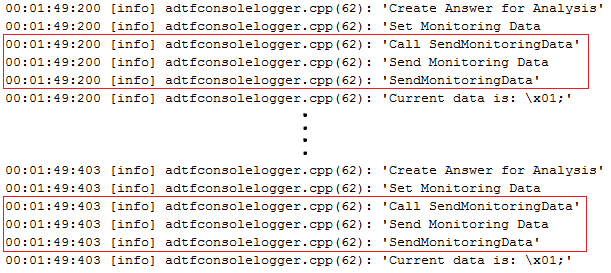
\includegraphics[width=1\linewidth]{Darstellungen/MonitoringTakt}
\caption{Konsolenausgabe ADTF beim Monitoring}\label{pic:Konsolenausgabe Monitoring}
\end{center}
\end{figure}
Zuletzt muss das Zusammenspiel mit dem Online-Analyse-Filter überprüft werden. Dessen Umsetzung ist kompliziert und die parallele Umsetzung brachte ein Modul mit Grundfunktionen hervor. Aktuell ist es noch nicht möglich, die abgespielten CAN-Bus-Daten auszuwerten, da es noch kein Modul zum Auslesen der Daten gibt. Allerdings ist das Filter schon in der Lage, die gesendeten Kommandos zu bearbeiten und sich nach den Vorgaben zu verhalten. Gemeint ist damit, dass für die entsprechenden Modi bereits Nachrichten im richtigen Format und mit der richtigen Taktung\footnote{einfaches oder wiederholtes Senden} an den UDP-Server gesendet werden. Die Messdaten entsprechen somit noch nicht den realen gemessenen Werten, aber es werden sozusagen Platzhalter gesendet.

Diese Grundfunktionalität genügt allerdings bereits, um die Interaktion mit dem Filter zu testen. Prinzipiell spielt es für den ADTF Adapter keine Rolle, welche Messdaten gesendet werden, so lange sie im richtigen Nachrichtenformat empfangen werden.

Besonderes Augenmerk beim Test liegt auf dem Test der Modi mit Messwerterfassung (Monitoring), da für diese Funktion eine spezielle Thread-Architektur entworfen wurde. Wichtig ist hierbei, dass die gewünschte Taktung eingehalten wird. Momentan ist eine Taktung von 0,2 Sekunden zwischen den Messwertdatenpaketen vorgesehen. Bei der Auswertung dieses zeitlichen Aspektes erweist sich die Funktionsweise der Konsolenausgaben in ADTF als besonders hilfreich. Zusätzlich zur ausgegebenen Nachricht wird auf der Konsole ein Zeitstempel angegeben. Dieser Zeitstempel bezieht sich auf den Start von ADTF. Durch eine Nachricht direkt vor dem Senden der Daten, kann sichtbar gemacht werden, dass der Abstand zwischen zwei Konsolenausgaben in etwa der gewünschten Zeitspanne entspricht (s. Abb. \ref{pic:Konsolenausgabe Monitoring}). 
\chapter{Zusammenfassung}\label{chap:Zusammenfassung}
Dieses Kapitel soll dazu dienen, die Arbeitsergebnisse zusammenzufassen und abschließend zu bewerten. Außerdem soll ein Ausblick über zukünftige Verbesserungen und Erweiterungen gegeben werden.
\section{Zusammenfassung und Bewertung}\label{sec:Zusammenfassung und Bewertung der Arbeiten}
Ziel dieser Arbeit war die Entwicklung eines Moduls aus dem Konzept des ADAS Test Systems. Dieses System soll den Fahrer bei der Durchführung einer Testfahrt für ein Fahrerassistenzsystem unterstützen. Im Detail soll das zu entwickelnde Modul die Datenaufzeichnung und die zeitgleiche Analyse von Fahrzeugdaten unterstützen.

Um das Arbeitsziel abzustecken, wurde zunächst eine Anforderungsanalyse durchgeführt. Diese Analyse fasst die umzusetzenden Funktionen des Moduls zusammen und definiert den Arbeitsumfang. Anschließend wurde ein Konzept für die Lösung der gestellten Aufgaben entwickelt und bis auf einen Teil danach umgesetzt. Bei dem in dieser Arbeit nicht umgesetzten Teil handelt es sich um das Modul zur zeitgleichen Auswertung der Messdaten. Das Arbeitsergebnis ist somit das Konzept für das Measurement Device und das Ergebnis der Implementierung. 

Das Konzept sieht vor, dass auf einem Messrechner die Software ADTF installiert ist. Diese Software dient dazu, die anfallenden Messdaten aufzuzeichnen, bietet aber durch eine speziell dafür entwickelte Komponente (Filter) die Möglichkeit, Messdaten während der Messung auszuwerten. ADTF soll durch ein Tablet, das die Benutzerschnittstelle zum Testfahrer bildet, gesteuert werden. Durch die Scripting-Schnittstelle von ADTF (für Python-Skripte) kann dieses automatisiert werden. Unter Verwendung dieser Schnittstelle wurde ein Softwaremodul entwickelt, das die Kommunikation mit dem Tablet-Programm über das TCP-Protokoll unterstützt. In das TCP-Protokoll bettet sich ein den Anforderungen entsprechend entwickeltes Protokoll, das die Steuerung von ADTF ermöglicht, ein. Als Übertragungsform wurde WLAN gewählt. In Folge dessen müssen der Messrechner sowie das Tablet im gleichen WLAN-Netz sein, um miteinander kommunizieren zu können.

Der ADTF Adapter, der das Ergebnis der Implementierung darstellt, unterstützt sowohl einfache Steueraufträge für ADTF, als auch komplexere Aufgaben zur Unterstützung der Online-Analyse der Messdaten. Abhängig von der Art der Aufträge kann der ADTF Adapter die Grundzüge seines Verhaltens variieren. Besonders durch die Forderung aktuelle Messwerte auch auf dem Tablet darstellen zu können, verändert der Adapter sein Verhalten und wirkt sozusagen als "`Vermittlungspartner"' zwischen dem Online-Analyse-Filter und der App auf dem Tablet. Der Online-Analyse wurde au\ss erdem ein weiterer Modus hinzugefügt, der bei der Anforderungsanalyse nicht geplant war. Dieser Modus ist eine Verknüpfung der beiden geforderten Funktionen.

Der Test der durch den Adapter zur Verfügung gestellten Funktionen ergab, dass alle Forderungen umgesetzt werden konnten. Der ADTF Adapter erfüllt genau jene Forderungen, die in der Anforderungsanalyse festgelegt wurden und bietet durch den dritten Modus zur Online-Auswertung eine weitere Funktion. Somit gliedert sich das Modul optimal in das Systemverhalten des ATS ein.
\section{Ausblick}\label{sec:Ausblick}
Trotzdem das entstandene Modul alle geforderten Funktionen erfüllt, gibt es Ansätze zur Erweiterung bzw. Verbesserung des Systems. 

Während der Erstellung des Konzeptes wurde auch Bluetooth als möglicher Übertra\-gungsmechanismus erwähnt (s. Kap. \ref{sec:ADTF Adapter}). Diese Möglichkeit wurde zunächst verworfen, aufgrund nicht abzusehender Probleme bei der Implementierung. Dennoch bietet die Verwendung von Bluetooth wesentliche Vorteile für das Gesamtsystem. Bei Verwendung von Bluetooth könnte auf den zusätzlichen WLAN-Router verzichtet werden, da dieser nicht nötig wäre. Die Bluetooth-Schnittstellen von Messrechner und Tablet könnten über Bluetooth eine direkte Verbindung aufbauen. Dies würde besonders im Fahrzeug von Vorteil sein, da der Router über das Fahrzeugbordnetz mit Strom versorgt werden muss. Eine Lösung mit Bluetooth würde somit wesentlich handlicher sein.

Die Generierung von Fehlertexten wird im ADTF Adapter durchgeführt. Das aktuelle Vorgehen wurde extra dafür ausgelegt, Mehrsprachigkeit zu unterstützen. Aus Zeitgründen wurde die Mehrsprachigkeit allerdings noch nicht umgesetzt und könnte in späteren Arbeiten hinzugefügt werden. Die Qualität der Fehlertexte könnte ebenfalls noch verbessert werden. Aktuell werden Fehler in den meisten Fällen zwar detektiert, aber die Ursache des Fehlers wird aktuell meistens nicht erkannt. ADTF selbst generiert in der Konsole bereits sehr aussagekräftige Fehlertexte, die durch den PSS allerdings nicht ausgelesen werden können. Über einen Umweg wäre es möglich, diese von ADTF generierten Fehlertexte abzufragen. Während der Laufzeit generiert ADTF eine "`log-Datei"', in der alle Konsolenausgaben gespeichert werden. Diese Datei könnte durch den ADTF Adapter geöffnet werden, um die Fehlermeldungen auszulesen, und diese dann an das Tablet zu senden.

Für den ersten Prototypen des Systems wurde eine vereinfachte Version implementiert, um prinzipiell die Umsetzbarkeit aufzeigen zu können. Dadurch ist das System in seinen Grundzügen noch relativ starr. In der aktuellen Umsetzung können beispielsweise nur die Daten eines CAN-Busses aufgezeichnet und analysiert werden. In der Praxis ist es allerdings eher üblich, dass mehrere Bus-Datenströme analysiert werden sollen. Um dies zu unterstützen, müsste vor allem die Konfigurationsdatei für ADTF dynamisch generiert werden können. Die Möglichkeit sollte zumindest überprüft werden, ob es sinnvoll ist, diese Konfigurationsdatei vom ADTF Adapter generieren zu lassen. Dazu müsste der Adapter die entsprechenden Informationen vom Tablet erhalten. 

Aktuell ist es noch nicht möglich, eine Auswahl über das zu verwendende dbc-File zu treffen. Der Pfad zu dieser Datei ist momentan ein fester Wert, der in der Konfigurationsdatei von ADTF gespeichert ist (Parameter des Online-Analyse-Filters). Kann diese Variable verändert werden, so können auch verschiedene Fahrzeugtypen durch das Testsystem unterstützt werden. Um diese Funktion umzusetzen, müsste das Protokoll zwischen ADTF Adapter und TDA verändert werden sowie die entsprechenden Operationen im Adapter umgesetzt werden.

Um die Sicherheit des Systems zu verbessern, wurde im Protokoll die laufende Nummer eingefügt. Über diese Nummer wird momentan sichergestellt, dass der ADTF Adapter die richtige Antwort auf die richtige Anfrage sendet. Der TDA überprüft die laufende Nummer darauf, ob das gesendete Paket zum gestellten Auftrag passt. Der TDA akzeptiert dann nur Pakete mit der entsprechenden Nummer, auf die Antworten gesendet werden dürfen. Aktuell besitzt der ADTF Adapter allerdings keine Überprüfung. Das aktuelle Verhalten sieht vor, dass es keine Übertragungsprobleme mit komplettem Paketverlust gibt, da das TCP-Protokoll zur Fehlererkennung und -behebung bereits entsprechende Ma\ss nahmen trifft. Über die laufende Nummer wäre es allerdings möglich, weitere Kontrollmechanismen zu implementieren. Der ADTF Adapter könnte beispielsweise aus einer übersprungenen Nummer ein verlorenes Paket identifizieren und könnte dann eine gezielte Anfrage nach dem fehlenden Paket senden.

Das Protokoll zwischen dem ADTF Adapter und dem TDA sieht vor, dass der ADTF Adapter Nachricht senden kann, wenn ein Systemfehler erkannt wurde. Solche Systemfehler werden aktuell noch nicht abgefragt. Es müsste ein geeignetes Konzept entworfen werden, um Fehler zu erkennen und dafür entsprechende Nachrichten zu generieren.
\begin{thebibliography}{99}
\bibitem{AEV}
Audi Electronics Venture GmbH: ADTF, Software-Umgebung für Applikationen und Tools, http://www.audi-electronics-venture.de/aev/brand/de/leistungen/
\\\ Entwicklungstools/adtf.html (Zugriff am 23.12.12)
\bibitem{ADTFDokuUsers}
Elektrobit: ADTF 2.7 Users's Manual, Elektrobit Group Plc., Erlangen, 2011
\bibitem{ADTFDokuDevelopers}
Elektrobit: ADTF 2.7 Developer's Manual, Elektrobit Group Plc., Erlangen, 2011
\bibitem{ADTFDokuSDK}
Audi Electronics Venture GmbH: ADTF 2.7 SDK Documentation, Audi Electronics Venture GmbH, 2012
\bibitem{PythonOrgExecutiveSummary}
Python Software Foundation: What is Python?, Executive Summary,
\\\ http://www.python.org/doc/essays/blurb/ (Zugriff am 29.12.2012)
\bibitem{GalileoPython}
Peter Kaiser, Johannes Ernesti: Python, Das umfassende Handbuch,
\\\ Galileo Press, Bonn, 2007, ISBN 978-3-8362-1110-9, Weblink zum Openbook 
\\\ http://openbook.galileocomputing.de/python/
\bibitem{ElkoTCP}
Patrick Schnabel: Netzwerktechnik-Fibel, Grundlagen Übertragungstechnik TCP/IP 
\\\ Dienste Sicherheit, Books on Demand Gmbh, Norderstedt, 2004, ISBN 978-3-8334-
\\\ 1681-1, Weblink TCP  http://www.elektronik-kompendium.de/sites/net/0812271.htm (Zugriff am 28.12.2012)
\bibitem{MasterEckerlebe}
Christoph Eckerlebe: Masterarbeit: Automatisierungsschnittstelle und Python Support Service für ADTF, FH Hildesheim Holzminden Göttingen, WS 2010/11
\bibitem{BernerMattnerMessina}
Berner \& Mattner Systemtechnik GmbH: Messina,
\\\ http://www.berner-mattner.com/de/berner-mattner-home/produkte/messina/
\\\ index.html, (Zugriff am 29.12.2012)
\bibitem{VectorDBC}
Vector Informatik GmbH: DBC-Kommunikations-Datenbasis für CAN,
\\\ Das Rückgrat von verteilten Kommunikations-Systemen, 
\\\ http://www.vector.com/vi\_candb\_de.html (Zugriff am 30.12.2012)
\bibitem{CANFederl}
Anton Federl, Serein Pfeiffer: CAN (Controller Area Network), Kommunikation im Automobil, http://www.anton-federl.de/pdf/DakoAusarbeitung.pdf
\\\ (Zugriff am 01.01.2013)
\bibitem{WikipediaPort}
Wikimedia Foundation Inc., Wikipedia: Port (Protokoll), 
\\\ http://de.wikipedia.org/wiki/Port\_\%28Protokoll\%29
\\\ (Zugriff am 30.12.2012)
\bibitem{IETFRFC6335}
Internet Engineering Task Force: Request for Comments 6335, 2011,
\\\ Weblink: http://www.rfc-editor.org/rfc/pdfrfc/rfc6335.txt.pdf
\\\ (Zugriff am 30.12.2012)
\bibitem{WikipediaASCII}
Wikimedia Foundation Inc., Wikipedia: American Standard Code for Information Interchange, http://de.wikipedia.org/wiki/ASCII (Zugriff am 06.01.2013)
\bibitem{OestereichUML}
Bernd Oestereich: Analyse und Design mit der UML 2.5, Objektorientierte Softwareentwicklung, Oldenburg Verlag, München, 2012, ISBN 978-3-486-71667-2
\end{thebibliography}
\appendix
\chapter[Anhang]{}
\newpage
\section{Verwendete Software}
Folgende Software wurde für die Bearbeitung der gestellten Aufgabe verwendet:
\begin{itemize}
\item{ADTF 2.7.1}
\item{Python 2.6}
\end{itemize}
\section{Inhalt der Disc}
Auf der beiliegenden Disc befinden sich folgende Daten:
\begin{itemize}
\item{Quellcode des ADTF Adapters}
\item{digitale Version dieser Arbeit}
\item{Kopien der Quellen}
\item{Testprotokoll für den Test des PSS}
\item{Unterlagen zum Testkonzept Fahrerarbeitsplatz}
\end{itemize}
\newpage
\section{Bedienungsanleitung}
In dieser Bedienungsanleitung wird schrittweise erklärt, wie der entwickelte ADTF Adapter verwendet wird.
\\[0.5cm]
1. Als erstes sollte der Quellcode, der sich auf der beiliegenden Disc befindet, in einem lokalen Verzeichnis des Messrechners abgelegt werden. Anschlie\ss end müssen einige kleine Änderungen am Quellcode vorgenommen werden.
\\[0.5cm]
2. Für die Kommunikation muss die IP-Adresse im Skript geändert werden. Mit der IP-Adresse ist die IP-Adresse der Netzwerkkarte (WLAN) des Messrechners gemeint. Diese muss zunächst ermittelt werden. Der einfachste Weg diese herauszufinden, ist den Befehl "`ipconfig"' über die Eingabeaufforderung (cmd.exe) von Windows einzugeben. Unter der Auflistung "`Drahtlos-LAN-Adapter Drahtlosnetzwerkverbindung"' ist die IP-Adresse unter dem Punkt "`IPv4-Adresse"' angegeben. Dieser dort abgelesene Wert muss in das Skript eingetragen werden. Dazu muss das Skript "`ADTF\_Adapter.py"' in einem Texteditor geöffnet werden. Folgende Codezeilen müssen am Anfang des Skriptes gesucht werden. 
\begin{quote}
\verb|Port = 55555|\\
\verb|IPAddress = "10.40.10.97"|\\
\verb|CommunicationInterface = TCP|\_\verb|Server.TCP|\_\verb|Server(ADTF,"IPAddress",Port)|\\
\end{quote}
Bei der Bearbeitung eines Python-Skriptes ist strikt darauf zu achten, die Einrückung nicht zu ändern, da diese wichtig für die Codestruktur sind. Für die Variable "`IPAddress"' muss der abgelesene Wert der Netzwerkkarte eingetragen werden.

Eine Grundvoraussetzung für die Funktion des ADTF Adapters sind die Firewall-Einstellungen des Messrechners. Um die Kommunikation zu ermöglichen muss die IP Adresse sowie der Port 55555 freigeschaltet sein. Ansonsten werden alle Nachrichten vom TDA von der Firewall geblockt.
\\[0.5cm]
3. Um im ADTF Adapter die benötigten Klassen importieren zu können, muss angegben werden, in welchem Ordner sich die entsprechenden Python-Dateien befinden. Dazu muss am Anfang des Skriptes folgende Zeile gesucht werden:
\begin{quote}
\verb|os.chdir(r"Pfad zum Skript-Ordner")|\\
\end{quote}
\noindent Für "`Pfad zum Skript-Ordner"' muss hier der absolute Dateipfad angegeben werden, in den der ADTF Adapter in Punkt 1 kopiert wurde.
\\[0.5cm]
4. Nachdem die Bearbeitung abgeschlossen wurde, kann das Skript in ADTF eingebunden werden. Dazu muss ADTF gestartet werden. Folgend muss zunächst ein Ordner im Project Tree generiert werden. In diesen kann danach das Skript "`ADTF\_Adapter.py"' importiert werden. Die Vorgehensweise wird in der folgenden Abbildung dargestellt (s. Abb. \ref{pic:Importieren Python-Skript}).
\begin{figure}[H]
\begin{center}
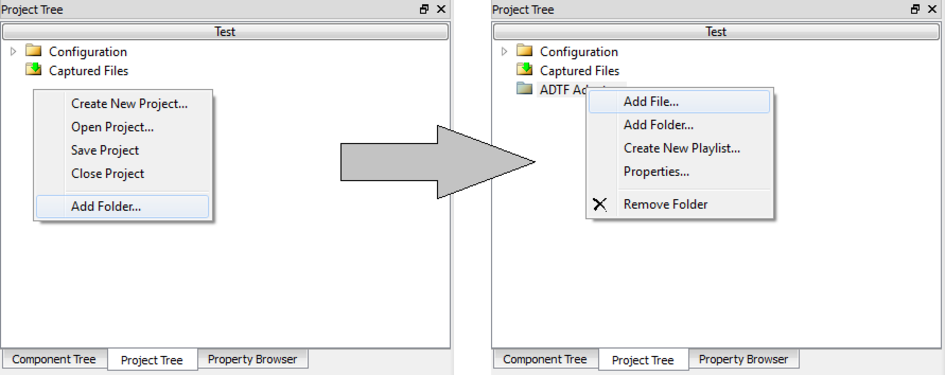
\includegraphics[width=1\linewidth]{Darstellungen/EinbindungSkript.pdf}
\caption{Importieren Python-Skript}\label{pic:Importieren Python-Skript}
\end{center}
\end{figure} 
\noindent 5. Nachdem das Skript importiert wurde, kann es durch einen Doppelklick gestartet werden. Der Adapter ist dann aktiv und wartet auf eingehende Verbindungsanfragen.
\addcontentsline{toc}{chapter}{Eidesstattliche Versicherung} %sorgt für eintrag ins inhaltsverzeichnis
\chapter*{Eidesstattliche Versicherung} %  *-> erstellt unnummeriertes chapter
%Hiermit versichere ich, Jens Noack, an Eides statt,  dass ich die vorliegende Bachelorarbeit mit dem Titel "`Entwurf und Implementierung eines Messsoftware-Adapters für ein Fahrerassistenz-Testsystem"' selbständig und ohne fremde Hilfe verfasst und keine anderen als die angegebenen Hilfsmittel benutzt habe. Die Stellen der Arbeit, die dem Wortlaut oder dem Sinne nach anderen Werken entnommen wurden, sind in jedem Fall unter Angabe der Quelle kenntlich gemacht. Die Arbeit ist noch nicht veröffentlicht oder in anderer Form als Prüfungsleistung vorgelegt worden.
Hiermit versichere ich, Jens Noack, an Eides statt, dass diese Abschlussarbeit von mir selbständig verfasst wurde. Es wurden nur die angegebenen Quellen und Hilfsmittel verwendet. Alle wörtlichen und sinngemäßen Zitate sind in dieser Arbeit als solche kenntlich gemacht.
\\[2cm]
\noindent\rule{0.35\textwidth}{0.3pt}\rule{0.2\textwidth}{0pt}\rule{0.45\textwidth}{0.3pt}
\\Ort, Datum\rule{0.418\textwidth}{0pt}Unterschrift
%\pagestyle{plain} 
%\section{Eidesstattliche Versicherung}
\end{document}